\documentclass[12pt,a4paper]{article}

\usepackage[dvips]{graphicx}
\usepackage[dvips]{color}
\usepackage{amsbsy, marvosym}
\usepackage{amsmath}
\usepackage{paralist}
\usepackage{wasysym}
%\usepackage{algorithm2e}
\usepackage{natbib}
\usepackage{algorithmic}
\usepackage{algorithm}
\usepackage{subfigure}
\usepackage{lscape}
\usepackage{booktabs}
\usepackage[cols=3,toc=true]{glossary}
%\usepackage{glossaries}
%\usepackage[acronym]{glossaries}
%\usepackage[toc]{glossaries}
\usepackage{lscape}
\usepackage[nottoc]{tocbibind}
\usepackage{setspace}

\newcommand{\HRule}{\rule{\linewidth}{0.5mm}}

\pagestyle{plain}
%\textwidth 16cm
\textwidth 14cm
\textheight 23cm
%\oddsidemargin -0.5cm
\oddsidemargin 2.0cm
\evensidemargin -0.5cm
\topmargin 0cm

%\linespread{1.6}

\numberwithin{figure}{section}
\numberwithin{table}{section}
\numberwithin{algorithm}{section}

\usepackage{float}
\floatstyle{ruled}
\newfloat{program}{thp}{lop}[section]
\floatname{program}{Program}

\newfloat{note}{thp}{lon}[section]
\floatname{note}{Note}

\newglossarytype[nlg]{notation}{not}{ntn}
\providecommand{\notationname}{List of Symbols}

\bibpunct{(}{)}{;}{a}{,}{,}
\makeglossary
%\makeglossaries
\makenotation


\begin{document}
\pagenumbering{arabic}
\setlength{\parindent}{5mm}
\setlength{\parskip}{10pt plus2mm minus2mm}
\thispagestyle{empty}
% TITLE

\begin{titlepage}

\begin{center}

% Upper part of the page
%\includegraphics[width=0.15\textwidth]{./logo}\\[1cm]

\textsc{\LARGE Liverpool John Moores University}\\[1.5cm]

\textsc{\Large Ph.D Thesis}\\[0.5cm]


% Title
\HRule \\[0.4cm]
{ \Large \bfseries Adaptive Optimal Telescope Scheduling}\\[0.4cm]

\HRule \\[1.5cm]

% Author and supervisor
\begin{minipage}{0.4\textwidth}
\begin{flushleft} \large
\emph{Author:}\\
Stephen \textsc{Fraser}
\end{flushleft}
\end{minipage}
\begin{minipage}{0.4\textwidth}
\begin{flushright} \large
\emph{Supervisor:} \\
Prof. Iain \textsc{Steele}
\end{flushright}
\end{minipage}

\vfill

% Bottom of the page
{\large \today}

\end{center}

\end{titlepage}

%\title{Adaptive Optimal Telescope Scheduling
%Ph.D Thesis}
%\author{S.N. Fraser}
%\date{\today}
%\maketitle


\begin{abstract}
Astronomical telescopes operate in a dynamic and uncertain operational environment. Time is often oversubscribed with programs competing for available slots and the best observing conditions. In order to achieve a high scientific return a scheduler must be able to create a globally optimal observing schedule. 

Using data collected from external sources and embedded instrumentation I investigate and characterize the scheduler's operating environment. I investigate metrics for characterizing the value of schedules both locally (at the decision point) and over longer horizons. Using this information an extensible software architecture is designed incorporating a simulation framework to allow a variety of schedulers and environmental scenarios to be constructed.

 Experiments are performed using the scheduler component architecture and simulation framework to determine the effects on schedule quality of environmental stability, disruptive events and reliability of prediction under a range of load conditions. 

%metrics 
Investigations into the effects of choice of selection scoring metric on the final quality of schedules showed that contrary to an initial opinion that it should be feasible to find a single candidate quality metric with which to evaluate schedule quality, there is in fact no clear candidate as an absolute quality metric. The choice of weighting of the selection metrics determines the character of the schedule but only the dominant scoring metric has any real effect while the other metrics simply manifest themselves as noise.

%stab reliable 0.7/0.8
It was found that where conditions are relatively stable there is an advantage to using longer look-ahead horizons but that where conditions are unstable or disruptive a basic despatch scheduler achieves results as good or better. A look-ahead scheduler with a horizon of 4 hours can give an improvement of upto 23\% over a simple despatch scheduler when seeing remains stable over a period of upto 6 hours.

Experiments performed to determine the effect of chosing a suitable look-ahead horizon based on the perceived stability of environmental conditions have shown that when determining the length of this horizon, if we either over or under-estimate the duration of stable conditions we obtain poorer results. When the stability length is severely under-estimated a loss of between 5\% and 17\% in quality was found to occur.  The optimum situation appears to be when the horizon is of order of or slightly less than the actual stability length. Where the stability length is over-estimated by a factor 2, a loss of 5\% to 10\% can occur.




\end{abstract}


\settocbibname{Bibliography}

\newpage
\tableofcontents
\newpage
\listoffigures
\newpage
\listoftables
\newpage
\listofalgorithms
\newpage
\printglossary
\newpage
\printnotation
\newpage

\part{Background}
% INTRODUCTION
\section{Introduction}
\label{sect:intro}

\subsection{Background}
\label{sect:intro_background}
% about the telescope
The Liverpool Telescope (LT\glossary{name={LT},description={The Liverpool Telescope}}),\citep{steele04liverpool} is a fully robotic 2 meter astronomical telescope situated at the Observatorio de los Roches de los Muchacos \glossary{name={ORM},description={Observatorio de los Roches do los Muchachos}} on La Palma in the Canary Islands ($28^{\circ}45N$, $17^{\circ}52W$) at an elevation of 2400m. It operates without supervision, controlled by an integrated suite of software systems \citep{fraser02robotic, steele97control}. 

% operating environment
The telescope operates in an uncertain environment:- \begin{inparaenum}[(\itshape i\upshape)] \item availability is influenced by weather conditions (it does not open when there is rain, high humidity or extreme or gusting wind), \item at times telescope operations may be \emph{taken over} by external agents \citep{mottram06high, allan04estar} to investigate \emph{targets-of-opportunity}, \item essential engineering work must be scheduled at various times, \item there are the inevitable and unexpected downtime due to software and hardware faults, \item atmospheric conditions which constrain the choice of available observation can change over short timescales, \item observation requests can arrive in the database or be removed or modified at any time \end{inparaenum}.

% how it works
The telescope's Robotic Control System (RCS\glossary{name={RCS},description={Robotic Control System}}) is responsible  for deciding on the mode of operation and for protecting the telescope. It controls the telescope and its instruments and monitors environmental information from a number of lower level subsystems. The observation program followed by the RCS is determined by the Observation Planning and Scheduling System (OSS\glossary{name={oSS},description={Observation Scheduling System}}) based on information in the Phase 2 Observation Database (ODB\glossary{name={ODB},description={Phase 2 Observation Database}}).

%\glossary{name={},description={}}

% ODB
The ODB contains details of observations specified by astronomers who have been allocated time by one of several Telescope Allocation Committees/Groups (TAC/TAG)\footnote{The 2 terms are synonymous, TAG is more usual in UK, TAC in USA}.
The term \emph{group} (Fig.~\ref{fig:group}) is used to describe the observation specifications. These contain details of what and how to observe (\emph{sequence}), when to observe (\emph{timing constraints}) and under what conditions (\emph{observing constraints}). 

% fig:group 
\begin{figure}[htbp]  
  \begin{center}
    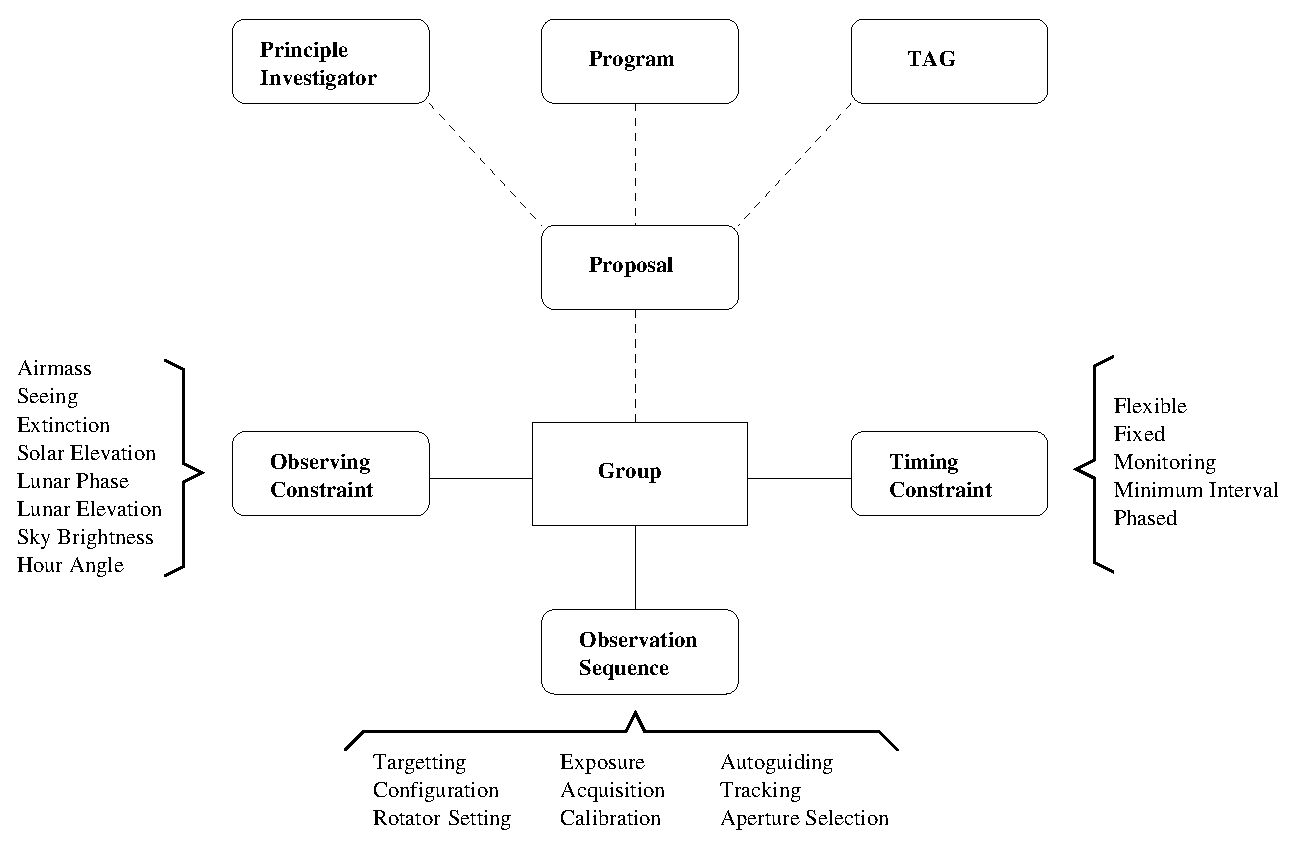
\includegraphics[scale=0.6, angle=0]{figures/group_structure.eps}
  \end{center}
  \caption[Structure of the Phase2 Observing Database (ODB).]
   {Structure of the Phase2 Observing Database (ODB). A \emph{group} contains all the information required to schedule and execute a series of observations. The \emph{observation sequence} contains details of the operations to be performed (target, exposure, instrument selection). \emph{Timing constraints} determine when the group may be executed. \emph{Observing constraints} determine under which atmospheric and other conditions the group is feasible. Groups are contained within a \emph{proposal} containing details of the science program and time allocations from its sponsoring TAG. Each proposal has a \emph{Principle Investigator} who is responsible for entering the observation details  .}
  \label{fig:group}
\end{figure}

% how does the initial OSS work
The current OSS deployed at the telescope \citep{fraser04scheduling} was developed based on the assumption that a despatching scheduler would be best at matching the varying conditions on site with the timing and observing constraints of the available groups. A despatch scheduler works by scanning the set of available groups. Each group which is determined to be feasible (with respect to the current conditions) is assigned a score. Typically, the group with the highest score at that moment in time is then selected for execution.


%\begin{algorithmic}
%\caption{Despatch scheduler algorithm}
%\FORALL{group in ODB} 
%\IF{$feasible(group)$} 
%\STATE $candidates \Leftarrow group$
%\ENDIF
%\ENDFOR

%\REQUIRE $maxscore \gets -99$
%\REQUIRE $best \gets null $
%\FORALL{group in candidates}
%\IF {$score(group) \geq maxscore$}
%\STATE $maxscore \gets score$
%\STATE $best \gets group$
%\ENDIF
%\ENDFOR
%\RETURN best
%\end{algorithmic}

\subsection{Planning and scheduling}
\label{sect:pandstimescales}
The terms planning and scheduling are often confused and indeed used interchangeably. They are however basically different aspects of the same process.
Planning is typically considered to be a long term activity taking a global view of an enterprise. It may set targets or goals to be achieved by the enterprise. These may be somewhat imprecise or abstract - we are not deciding \emph{what} to do and \emph{when} so much as what \emph{sort} of things we want to do and \emph{how well} we want to achieve them. Scheduling on the other hand deals with the rather more precise objective of assigning actual resources to accomplish specific tasks at specific times.

The planning \emph{horizon} is the period over which a plan is made or is expected to be of some utility in achieving its set of goals. In practice we can usefully subdivide planning into several different levels characterized by their horizons \citep{haxhierarchic73}. The subdivisions are by no means set in stone and more or fewer horizons may be more suited to specific enterprises. As we move down the hierarchy, typically, the precision of the objectives becomes more focused and the horizon time span decreases \citep{chien00aspen}.

\begin{description}
\item[Strategic] planning involves the creation of plans to cover very long periods of time. In the current context this could be a semester of telescope time, and more generally could at its most extreme represent the entire lifetime of an enterprise. 
\item[Tactical] plans are designed to cover medium periods e.g. a lunar cycle or half cycle on a telescope,  weekly or monthly production targets in a factory.
\item[Operational] plans \footnote{may also be refered to as \emph{Mission planning}} are short term plans designed to allow an enterprise to function on a day to day basis. Typically they cover the \emph{standard} work-period of the enterprise e.g. a night's observing at a telescope, a shift at a factory.
\item[Scheduling] Takes place over a short period and deals with the specific assignment of resources to tasks. This could range from determination of just the next observation upto the specification of the sequence of observations over the next few hours.
\end{description}

In this thesis we shall consider only the problem of scheduling. Though levels of planning may be incorporated into a final operationally deployed system they are likely to manifest themselves through adjustment of the relative weightings of the quality metrics used by the schedulers over periods longer than a night. 


% e.g. in the form of objective functions or the specification of constraints and preferences to be considered by lower layers. 

\subsection{Motivation}

This system has been in operation now for 7 years since the telescope went on sky (2004) and has performed adequately, however a number of criticisms can be made concerning this implementation.

\begin{itemize}

%\item [obscuration] Due to the objective function scoring mechanism it is not usually clear at any time why a particular group is favored over others or whether a specific group is likely to be selected at a given time. We cannot event tell which group might be selected next.

\item There is no \emph{commonly agreed} mechanism for measuring what represents a \emph{good} schedule (but see \citep{steele97control}). In order to compare the results of different scheduling implementations we need some means of determining the value or reward associated with a schedule. This can be considered from 2 points of view. For the user, the highest reward is likely to be achieved if his observations are made regularly, at the most favourable times with respect to the timing constraints and under the most favourable environmental conditions. For the enterprise, the highest reward might be achieved if the observations selected are most \emph{valuable} in terms of TAG assigned priority and may require some degree of program completeness to be sasified .

\item We do not have a detailed understanding of how conditions change on site and how this might affect planning and scheduling. At present no consideration of environmental change is considered in the planning and scheduling process. Similarly there is no real understanding of the effects on scheduling of the potentially rapidly changing content (volatility) of the ODB.

\item Despatch schedulers have been described as \emph{myopic} \citep{cicirello01random}, in that they select the \emph{best group} to execute at a point in time without reference to what might lead to an overall good schedule. There is no consideration of whether a better sequence might be generated by looking ahead a few steps. This is an example of \emph{local} rather than \emph{global} optimization.
%\item difficult - how do we select the best relative weighting for metrics?.

%\item [efficiency] The current scheduler must be invoked on demand whenever the RCS has completed a group and must then search through the entire ODB to determine which groups are feasible, score these and determine the current best group. 

\end{itemize}

It was therefore decided to conduct a series of experiments using different scheduler paradigms in order to determine how these would perform under a range of environmental and load scenarios.

\subsection{Plan}

The thesis is divided into 2 parts. In the first part, information is gathered to measure and characterize the operating environment and then used to design a scheduling architecture. 

\begin{enumerate}
\item In Sect.~\ref{sect:metrics} an investigation is made into the subject of metrics and reward. Two types of metric are considered. Complexity ($C$) metrics are applied to the measurement of ODB characteristics. These indicate how \emph{difficult} a particular scheduling problem might be. Quality ($Q$) metrics are used to measure the reward or value of a generated schedule and allow a comparision between the success of different scheduler implementations or between different problem sets. 

\item Software embedded within the current robotic control system and scheduler is used to collect information relating to the characteristics of the telescope's operating environment. This information is analysed in Sect.~\ref{sect:character} to determine whether it will be possible to incorporate predictions of environmental conditions into decision making. 

\item Information gathered in the 2 preceding stages is used to design an architecture with which to build a variety of scheduler and planner implementations and incorporating components with which to construct simulation environments to test these schedulers. Heuristic scoring ($f$) metrics are employed by the scheduler and planner implementations to perform search and optimization processes. Mitigation of the effects of changing conditions are considered by looking at the concept of discounted future reward. The scheduler architecture is described in Sect.~\ref{sect:architecture} with further details of the simulation components in Sect.~\ref{sect:experiments}.
\end{enumerate}

In the second part of the thesis a number of simulation experiments are performed using the framework described in Sect.~\ref{sect:architecture}

Two different types of scheduler are considered. The \emph{despatch} scheduler, as currently operationally deployed works by considering which of the various feasible candidates achieves the best score under a particular scoring model at the current time under the current conditions. The \emph{look-ahead} scheduler examines a number of feasible sequences of observations starting from the current time and looking forward by a single horizon length. It compares each sequence selecting the one which maximizes the potential reward.

\begin{enumerate}
\item In Sect.~\ref{sect:mam_study} a human scheduler is pitted against a simple despatch scheduler to act as a shakedown for the framework and to provide a baseline against which to test further schedulers.

\item The effect of varying the weights of the various scoring metrics on schedule quality is tested in Sect.~\ref{sect:exp_scoring}.

\item An investigation into the scale and range of Phase 2 loading is made in Sect.~\ref{sect:exp_complexity}. Schedulers are tested against generated Phase 2 models of differing complexity to determine how this affects scheduling performance.

\item Experiments are performed in Sect.~\ref{sect:exp_stability} to investigate the effect of variable environmental stability on schedulers and to determine which schedulers if any perform best under differing stability regimes.

\item Various unpredicted disruptive events can take place during a night's observing. An investigation into the effects of these disruptive events on schedule quality is made in Sect.~\ref{sect:exp_disruption}.

\item When the content of the Phase 2 ODB is changed during the course of the observing night there is likely to be some effect on scheduling. A detailed study of the effects of Phase 2 volatility are investigated in Sect.~\ref{sect:exp_volatility} in order to determine their effect on scheduling quality.


\item Look-ahead schedulers must decide at some point on how long a forward horizon they should use. In Sect.~\ref{sect:exp_reliability} simulations are performed to investigate how the reliability of determination of such horizon lengths based on environmental stability criteria affects these schedulers.


%\item Develop a despatch scheduler as a baseline with which to test more advanced schedulers, Tune the baseline scheduler using various controllable parameters, typically objective weighting functions and bias function, to investigate the limits of this scheduling paradigm in the telescope scheduling context.

%\item As the basis for the final system, I will develop a look-ahead scheduler incorporating (really !!) short-term prediction of environmental statistics to allow advanced planning of observations and using feedback of performance to adjust the plan objectives.

%\item Investigate variation of scheduling control parameters and horizon length on quality of schedules generated under varying environmental models to determine how to adapt to these - teh quality of schedules generated will be compared to those geenrated by the baseline system working at its maximum efficiency.

%\item Knowledge gained from this investigation will be incorporated into a final adaptive, look-ahead scheduler.
\end{enumerate}


% LITERATURE REVIEW
% ----------------------------------------------------------------------------------
% REVIEW OF LITERATURE
% ----------------------------------------------------------------------------------
%\chapter{Review of current research}
\section{Review of current research}
\label{sect:review}

%Survey and critical assessment. Relation to own work.

%Various topics in scheduling literature:-

%Online versus offline. Constructive/partial ordered versus iterative,repair based. Flexible schedules.  Search in scheduling. Integrated S+P. Techniques - CSP, agent-based/distributed, evolutionary/bio-inspired/ais, economics/markets, rlt.




 %At any point a usable if non-optimal schedule can be extracted by removing unassigned tasks so the technique is applicable in dynamic environments - i.e. reactive repair. NOT TRUE unless we have consistent schedule at that point.


%Whichever technique is employed the solution will involve a search over the potentially extremely large space ${D_1 \times D_2 \times \cdots \times D_n}$.  The terrain of this search space can prove be very rugged - \cite{beck97texturebased} have suggested the use of texture based metrics to characterize the structure (short examples)- (and see ref therein to original paper by M. Fox). 

There is a vast literature on the subject of scheduling covering both generic problems and highly domain-specific problem areas. In this section I present a brief introduction to some general techniques and review a number of specific case-studies. 

The constructive and iterative schedule building paradigms are introduced in Sect.~\ref{sub:review_constructive} and Sect.~\ref{sub:review_iterative} respectively. Sect.~\ref{sub:review_search} details a number of search techniques used to speed up the scheduling process. A number of individual case studies are described in more detail in Sect.~\ref{sub:review_casestudy}. Flexible and reactive scheduling methods are described in Sect.~\ref{sub:review_flexible}. In Sect.~\ref{sub:review_agent} a number of agent-based distributed scheduling systems are discussed.  A number of biological and evolutionary based scheduling paradigms is described in Sect.~\ref{sub:review_bio}. The use of artificial intelligence (AI) techniques including adaptive learning methods are described in Sect.~\ref{sub:review_adaptive}. 


% CONSTRUCTIVE
\subsection{Constructive techniques}
\label{sub:review_constructive}

The constructive approach to generating schedules starts from an empty schedule, progressivly selecting tasks to assign to vacant time slots, gradually building up the schedule. Effectively it generates a path through the search space. As the search progresses, dead-end points may be reached where some task becomes unassignable. The search must then backtrack, unwinding previous assignments and attempting to reassign tasks in order to avoid these dead-ends. An uninformed search can be very inefficient, however, search performance can be improved by using domain knowledge to derive heuristics (rules of thumb) via some of the following techniques:- 

\begin{description}
\item[Variable ordering heuristics]
determine the order in which variables \footnote{In this context, \emph{variable} refers to some resource which is to be allocated. In this thesis we will be concerned with a single variable \emph{time}.} are selected for assignment. In scheduling this corresponds to the order in which tasks are selected for time-slot assignment. The \emph{minimum remaining value} (MRV) heuristic \citep{bitner75backtrack} always selects the variable with the fewest legal assigments to place next, causing the search to fail fast and allows rapid pruning of the search tree. \citet{sadeh91lookahead} describes a number of variable ordering heuristics used in the MicroBOSS scheduler. These are split into \emph{fixed variable order heuristics} where the order is predetermined at the start of the search and \emph{dynamic variable order heuristics} where the order is revised each cycle. The \emph{MinimumWidth} heuristic selects the variable with the fewest arcs, i.e. constraint associations with other variables. Their \emph{operation resource reliance} (ORR) variable order heuristic selects the task which relies most on the most contended resource or time period. In the \emph{MinConflicts} heuristic \citep{minton92minconflicts}, at each point in the search a variable is selected which is in conflict and its value is adjusted until it is no longer in conflict. 

% Also \emph{maxflex} (myers) and \emph{mincontention} maybe in IR section?)  THESE ARE RETRACTION HEURISTICS !!

\item[Value order heuristics]
determine how the value is chosen to assign to a selected variable. \citet{sadeh91lookahead} describes a \emph{filtered survivable schedules} (FSS) heuristic which assigns to an operation the time-slot which is likely to be compatible with the largest number of survivable schedules or chances of surviving competition with other operations for possession of a resource. The technique empoyed detects \emph{cliques}, areas of the constraint graph with the tightest constraints. They also describe a mechanism to allow the scheduler to switch to a simpler (cheaper) value order heuristics when contention drops below a threshold.
% This concept of \emph{texture} of the search space is investigated in detail by \cite{beck97texturebased}.

%(Note:simplify the detailed decription in section 6 of the article - concentrate on cliques (clumpings) where graph has tightest constraints = texture heuristics also \cite{beck97texturebased} ). (Note: A couple more examples).

\item[Constraint propagation]
A more general improvement can be made using constraint propagation techniques. Here the implications of a constraint on a variable are tested against the constraints on other connected variables. For arc-consistency there must be a consistent assignment of variables to $X$ for every valid assigment of connected variable $Y$, if not we must delete values from one or other domain. The effects are then propagated to neighboring arcs. The name stems from the way new constraints are inferred and added to the constraints set. $k$-consistency takes this further by insisting that for every $k-1$ assigned variables a consistent value can be assigned to any $k^{th}$ variable. Conflict analysis though costly (typically $O(e^n)$) \citep{bitner75backtrack} can reduce backtracking by pruning the search tree. There is a trade-off in the time taken to perform the consistency checking and the reduction in problem size generated.

 In \citep{johnston94spike} the use of node ($k=1$), arc ($k=2$)and path ($k=3$) consistency is used to prune the search space for scheduling observations with the Hubble Space Telescope (HST). An example of arc-consistency between binary-constrained variables is given where two observations $A$ and $B$ with a precedence constraint $B$ \emph{after} $A$ by at least $\Delta t$ with each observation having unit duration (for simplicity) and restricted to the interval $[t_A,t_B]$ then the sub-interval $[t_A,t_A+ \Delta t+1]$ is excluded from the domain for $B$ and the subinterval $[t_B-\Delta t-1,t_B]$ is excluded from the domain for $A$. The trade-off in time spent consistency checking against problem reduction is handled in SPIKE by enforcing a strict time-limit for this procedure.

\item[Deadend recovery heuristics] 
The occurance of deadends resulting in the need to perform backtracking indicates that the chosen variable and value ordering heuristics and consistency enforcing techniques are insufficent to cope with the problem in hand. Further, a consequence of re-application of these same heuristics on backtracking is that the same deadends may be encountered repeatedly, a thrashing effect. Recovery heuristics are designed to allow for more intelligent choice on how to backtrack. \citet{sadeh94backtracking} describes several general techniques for improving backtracking search using the \emph{partial conflict set} of the deadend (i.e. the set of activities which have blocked progress of the search at that point and which may have been involved in previous deadends).

\begin{itemize} 
\item \emph{Dynamic Consistency Enforcement} (DCE) keeps a history of backtracking events to identify resource critical subproblems and unwinds assignments until a consistent state is reached.
\item \emph{Learning Order from Failure} (LOFF) technique attempts to adjust the variable ordering heuristic on encountering a deadend by unwinding to a consistent state then overriding the default heuristic to assign the activities in the partial conflict set before those which would otherwise have been chosen.
\item \emph{Incomplete Backjumping Heuristic} (IBH) uses texture based measures \citep{beck97texturebased} to identify assignments which are estimated to lead to more global solutions so that when a deadend is detected unwinds to this critical assignment and tries alternatives - e.g. use second best assignment rather than best. 
\end{itemize}

\end{description}

A disadvantage of the constructive approach is its \emph{offline} nature. A schedule generated by any offline technique will generally be impossible to follow in dynamic environments for any length of time. During execution any breaks are likely to cause the whole schedule from that point onwards to have to be regenerated, perhaps frequently, at some cost in time and computing resources.

%
% Iterative Repair techniques
%
\subsection{Iterative repair}
\label{sub:review_iterative}
Iterative repair based scheduling starts with an initial, probably sub-optimal and possibly infeasible schedule solution. It then  attempts to repair this by iteratively swapping assignments using local search techniques. The repair operations may involve \emph{retraction heuristics} for determining conflicting or over-subscribed tasks to remove followed by the use of \emph{replacement heuristics} to determine which new assignments to make. 

Repair may occur as part of a search process to find an optimal schedule from a preliminary first guess. It may also be neccessary to repair in a reactive context to fix an already executing schedule. This might have been disrupted by unexpected changes to the environment or goals or used opportunistically to take advantage of such changes to increase the global value. A task might finish earlier than expected which could provide an opportunity to bring another task forward.

Several such retraction and task-swapping heuristics are described by \citet{kramer04swapping} and later in Sect.~\ref{sect:review_opis} of this review. 

%SEARCH

\subsection{Search techniques}
\label{sub:review_search}
Before embarking on a review of scheduling methodologies we will briefly examine some of the available search techniques which have been applied to scheduling. 


%A number of search techniques have been investigated in this field, ranging from mathematical optimization/ constraint satisfaction methods such as Linear and Integer Programming (LP, IP) (REFS eg. H-OPT), local search techniques (Greedy search/hill climbing)(REF), local search with noise (simulated annealing (REF), adaptive noise (REF)) problem-specific (and generic) heuristic methods (MTS, RBDS)(REF), AMP (REF) techniques such as (TABU (REF), scatter search (REF) , A*(REF), LRTA*(REF)), HBSS(REF), SWO(REF), WHISTLING(REF). 

We must first distinguish between local and systematic search. Local search is characterized by operating around a small neighbourhood of the search space. It is generally memoryless or has a very short memory.

Systematic search however generally contains some sort of memory of previous search areas, operates on a larger scale and includes the concept of global optimization.
% also some notes about representation for constructive and repair based scheduling methods.


\begin{description}
\item[Local search]
Typically this proceeds by making small moves around the \emph{current} neighbourhood in the search space. Various types of local search are characterized by the mechanism for selecting the \emph{move} operation. These heuristics or \emph{rules of thumb} are guided by specialized domain knowledge and often a degree of experimentation and tuning is required to achieve acceptable performance.

Greedy search also known as hill-climbing and as gradient descent depending on whether the aim is to maximize or minimize the objective, is a classic local search technique. The move operation steps one unit in the direction of highest upward (or downwards) change in objective function - i.e. we move up (or down) the hill following the steepest gradient. The search continues until the peak (or valley) has been found as quickly as possible. In smooth search spaces this can be a very effective technique, however where the search space has a \emph{rough} texture \citep{beck97texturebased, fox89constrained}, this search mechanism can become trapped at \emph{local} maxima (or minima) with no possibility of escape to allow the search to explore other parts of the space. If the roughness of a search space is well understood, and this is often difficult as search spaces are frequently multi-dimensional and not easily visualized then a local strategy may prove adequate. Often however the \emph{texture} of the space may well not be known in advance, so the effectiveness of local search heuristics can be limited. In an attempt to allow search mechanisms to escape these localization effects a number of techniques have been developed.

\item[Search with noise / stochastic local search]
In a typical scenario, a parameter $p$ is chosen so that on any search move, the probability of making an \emph{off-heuristic} move instead of the the move that would be chosen by the local search heuristic is $p$. The addition of noise allows the search to jump to new areas of the search space while finding potential local maxima. The amount of noise however is critical, too little and the search is trapped at local peaks. Too much and the search becomes random, missing the peaks. \citet{mcallester97evidence} state that the optimal stochastic noise parameter is dependant on the problem characteristics and on the detail of the search heuristic and that it is difficult and time-consuming to obtain an optimal noise for a given problem domain and that it may be influenced by features of a specific problem. They found that the progress of a search can be characterized by measuring the ratio of the mean to the variance of the objective function during the search and that this can allow tuning of the noise parameter more quickly than by the usual trial and error techniques.

\item[Simulated annealing]
First described by \citet{kirkpatrick83optimization}, simulated annealing (SA\glossary{name={SA},description={Simulated Annealing}}) is a technique based on the statictical mechanics of cooling of metals. During the search a random \emph{off-heuristic} move is chosen with a probability which depends both on the proximity of the objective for a neighbouring location and on a parameter $T$, the annealing temperature which is slowly decreased as the run progresses. Early in the search, the value of $T$ is such that larger jumps are taken, later the cooling process allows for only small jumps as the search closes in on the optimal location. In its original form the jump probability was determined by $e^{-\frac{f_o-f_x}{kT}}$ where $f_0$ is the current objective value, $f_x$ the objective value at a nearby point $x$ and $T$ the annealing temperature. The choice of cooling schedule, i.e. how quickly and in what manner $T$ decreases has some influence on the results and is a parameter which requires tuning.

 Alternative techniques have been advanced, include quantum annealing (QA\glossary{name={QA},description={Quantum Annealing}}) \citep{apolloni89quantum} based on the quantum tunnelling effect. Whereas in SA, the probability of a move out of a local minimum is dependant on only the height of the barrier and so high barriers can cause the search to become trapped, the tunnelling probablity in QA depends both on the hight and thickness of the barrier. QA is an attempt to handle search landscapes where shallow local minima are sourrounded by high, thin barriers as the search is capable of escaping from these traps.


\item[Adaptive noise]
A problem with using random noise in search is that the noise parameter must be tuned using a combination of domain specific knowledge and trial and error. Further it may well depend critically on a specific problem instance. To overcome this limitation, \citet{hoos02adaptive} developed an adaptive noise mechanism. They use a metric \emph{noise response} based on the distribution of run-times for typical runs of the search. Using this parameter they adapt the level of noise to the rate of improvement. In the early stages they use greedy search, but as the rate of improvement decreases, described as search stagnation, they increase the noise level. If no improvement is obtained the noise is further increased to try to escape local minima. Once improvement occurs the noise level is then quickly decreased again.

In the context of spacecraft operations scheduling using the ASPEN system, an adaptive noise mechanism based on that already described is employed by \citet{fukunaga04robust}. They state that the increase and decrease mechanisms are asymmetric. When stagnation occurs there is a delay in applying the noise, effectively while they build up evidence that there is a problem. Once improvements are detected however, the noise is removed at a faster rate than it was applied. They found that in typical scenarios the adaptive mechanism gave results close to those obtained by the static noise technique, though rarely better. In worst case scenarios, where the static noise technique gave poor results, the adaptive mechanism performed significantly better. They argue that in their domain, it is often better to mitigate against worste-case situations than to always obtain best-case results.

\item[Moving search]
In robotics a common planning problem involves finding a route between various nodes or destinations often with variable costs for the different route decisions. This can be extended to situations where some of the nodes move around or the costs vary over time. The problem is similar in nature to scheduling scenarios in which the goals vary in time. A number of search techniques have been developed for these problems including $A^*$ \citep{hart68formal}, a gradient descent method based on estimated distance to target and cost so far, $LRTA^*$ \citep{ishida96improving} an improved real-time version of $A^*$ which learns the costs of visited edges and uses this information to speed up the search. Moving Target Search (MTS) \citep{yokoo99search} is an enhanced algorithm in which the \emph{hunter} builds up heuristic knowledge of the edge costs to all the target locations as the \emph{prey} moves between them.

\item[AMP]
Adaptive Memory Programming \citep{taillard98adaptive} was first coined as a general term for a class of optimization techniques which use some form of memory to retain knowledge about poor parts of the search space which have been visited recently.

In TABU search \citep{glover99tabu}, as the space around a solution is searched a short term memory keeps track of locations which have been visited and which have not yielded optimal solutions, typically local minima, to avoid re-tracing into these areas. 

 %and avoids entering these 'taboo' areas. there is stuff in \cite{xxx} (one of the later nasa papers) about TABU plus SWO and HOPT for spacecraft ops - combined method using IP and heuristics.

In scatter search \citep{glover03scatter} new, fitter solutions are generated by evolving previously found solutions in a process similar to that used in Genetic Algorithms (GA\glossary{name={GA},description={Genetic Algorithm}}) in that parts of 'fit' solutions are combined to yield new solutions which may be expected to retain some of the 'fitness' of the parents. Unlike GAs, scatter search provides mechanisms for combining solutions using derived rules and an adaptive memory rather than making these decisions randomly.

\end{description}

% MAYBE MOVE TO END OF CHAPTER ??????? 
\subsection{Case studies}
\label{sub:review_casestudy}

\subsubsection{SPIKE}
The SPIKE scheduler \citep{johnston94spike} was originally developed for operation of the Hubble Space Telescope (HST). This is a complex scheduling problem involving the allocation of observing time to between 10000 and 30000 observations per year. There are a large number of operational constraints with timescales spanning 6 orders of magnitude. 

Planning and scheduling is split into two timescales. The long-term planner assigns activities to a week or part of a week in the HST operating cycle. The short-term scheduler makes the detailed assignment of activities within each week. The scheduler takes account of hard (feasibility) and soft (preference) constraints through the use of \emph{suitability} functions, numerical representations of the degree of preference of one constraint over another. 

SPIKE uses an iterative technique described as \emph{Multi-start Stochastic Repair} which operates a cycle of: \emph{Trial assignment} $\rightarrow$ \emph{Repair} $\rightarrow$ \emph{Deconflict}. During the \emph{Trial asssignment} phase, activities are assigned to time slots using simple heuristics such as \emph{MinConflicts} \citep{minton92minconflicts}. This results in a first schedule attempt which will most likely contain numerous constraint violations and will be sub-optimal. 

The \emph{Repair} phase attempts to eliminate constraint violations using a hill-climbing heuristic applied via a neural network. Finally the \emph{Deconflict} phase tackles any activities which are in conflict using simple retraction heuristics. The process is repeated over many cycles improving the schedule quality each time. Several quality metrics are used to asses the quality of schedules. These include: Number of observations, total observing time, summed degree of preference. 


\subsubsection{Partially Ordered Schedules (POS)}
\citet{muscettola92bottleneck} describes a system (Conflict Partition Scheduling or CPS) for solving scheduling problems by identifying regions of the search space where bottleneck conflicts occur, then posting constraints to move the search away from these regions where solutions are unlikely to be found. A bottleneck is defined as a neighbourhood in the search space where the time assignment strategy generates a maximum of inconsistency. These are detected by running a number of stochastic simulations to generate resource allocations with time flexibility. The bottlenecks are identified as those points where the most resource contention occurs. Additional sequencing constraints are then posted to reduce this contention. 

They employ two measures of contention. \emph{Activity demand} $\Delta(\tau,t_i)$ measures how much an activity $\tau$ relies on a time slot $t_i$ by counting the number of simulations in which $\tau$ was asssigned to $t_i$. \emph{Resource contention} $X(\rho,t_j)$ measures how many activities are competing for a resource $\rho$ at time $t_j$ by counting the number of simulations in which $\rho$ is requested during $t_j$. During this \emph{Capacity analysis} phase, various variable and value ordering heuristics are employed. These heuristics can be altered to suit the scheduling preferences to be enforced such as a preference towards early finishing.


%- FTD, BTD, RVS - DETAILS. Conflict resolution involves - (see their FIG-1 on p5 for algorithm). brief description (esp CPS) - (may not use this list just salient points).

They test against a micro opportunistic scheduler \emph{Microboss} \citep{sadeh91lookahead} and against \emph{Min Conflicts Iterative Repair} \citep{minton92minconflicts}. Relative to \emph{Microboss}, CPS produced more solutions, faster in the harder problem categories though on simpler problems it was slower to converge. Relative to \emph{MinConflicts}, CPS performed consistently better. In harder problem cases with more bottlenecks \emph{MinConflicts} performed very poorly in comparison to both \emph{Microboss} and CPS. 


\subsubsection{MicroBOSS}
The MicroBOSS scheduler is described in \citep{sadeh91lookahead}. The search cycle employs a look-ahead technique to work out a probabilistic demand profile. An \emph{Operation Ordering} heuristic determines the critical jobs associated with the  highest demand periods while a \emph{Reservation Ordering} heuristic ranks the costs incurred by these jobs and makes appropriate reservations. A consistency enforcement rule determines new constraints based on the reservations made in the cycle. Where dead-ends occur in the determination of a schedule, backtracking is employed to escape to a known consistent point.

 The micro-opportunistics search heuristics allow for constant revision of strategy during construction and repair. MicroBOSS is able to handle reactive repairs to an already partially executed schedule. The operations which need re-scheduling are removed from the existing schedule and new constraints determined based on the existing scheduled activities. The new sub-problem is submitted to microBOSS which determines a solution to add to the existing (running) schedule. In tests conducted against a series of despatching rules on a jobshop problem, MicroBOSS was found to be less expensive (around 20\%) in terms of the chosen cost function - a combination of tardiness and inventory costs. 


\subsubsection{Gerry}
\citet{zweben94scheduling} describe the GERRY system for scheduling space shuttle ground operations. They define 3 types of constraint:- \begin{inparaenum}[(\itshape a\upshape )] \item temporal constraints represent precedances between activities, \item resource constraints represent usage of resources and \item state constraints represent particular environmental state variable assignments required by some activities - certain activities, denoted as \emph{achievers} are able to set these variables \end{inparaenum}. A weighted penalty function is used to measure the cost of constraint violation. Their repair procedure considers each type of constraint seperately and handles repair of $N$ of each type per cycle before moving onto the next cycle. In order to avoid trapping at local optima in the search space they employ simulated annealing to determine acceptance of a newly generated schedule. At each iteration the cost of the current schedule $s$ is compared to the best so far $s^*$ and is accepted with a probability $P(s,s^*) = \exp{-\frac{|cost(s)-cost(s^*)|}{T}}$ where $T$ is the \emph{annealing temperature} which is cooled during the search. 

To resolve resource constraints, tasks are selected for repair using 3 heuristic criteria:- \begin{inparaenum}[(\itshape i\upshape )] \item \emph{fitness} - move the task whose resource requirements match the amount of over-allocation most closely - the logic here is that a task which has a small resource requirement is less likely to have much effect, one which has a very large requirement will cause problems wherever it gets moved to, \item \emph{dependency} - move the task which has the fewest temporal dependants - a task with a large number of dependencies will likely cause additional violations when it is moved and disrupt existing assignments, \item \emph{distance} - move the task which needs the smallest move to resolve the conflict - a large move is likely to perturb the overall schedule more.\end{inparaenum} The results of these metrics are scored and a task selected for the move. State constraints are repaired using a selection of 5 methods in priority order which involve moving the affected task and/or adding \emph{achiever} tasks into the schedule before the affected task to set the variable appropriately. The GERRY scheduler was found to be very effective in the chosen domain and was incorporated into the NASA Ground Processing Scheduling System (GPSS) an interactive tool for scheduling repair and refurbishment of the space shuttles between missions. 


\subsubsection{OPIS/OZONE}
\label{sect:review_opis}
\citet{smith95reactive} describes the OPortunistic Intelligent Scheduler (OPIS) system. This introduces multi-perspective scheduling in which a number of complimentary schedule repair techniques are employed under the supervision of a Top Level Manager (TLM) and working through a common blackboard representation of the current solution and constraints. External events (changes to requirements, feedback from execution) are fed into the blackboard via model update agents. 

Conflict classes are defined relative to a number of conflict metrics including:- conflict duration, conflict size, resource idle time, upstream slack, projected lateness. A number of agents analyse the conflicts which are then matched to fuzzy behavioural profiles. Schedule repair agents are then selected to apply an appropriate repair heuristic suited to the character of the conflicts. e.g. for a problem with HIGH value of \emph{conflict duration} and LOW value of \emph{variance in projected lateness} coupled with HIGH value of \emph{idle time} the \emph{order-scheduling} heuristic is chosen which revises the sequencing of contiguous operations. 

In the trade-off between opportunistic improvement and non-disruption to current baseline OPIS is biased towards the later though this is a function of the analysis and repair heuristics chosen.% -- see later under OZONE and DITOPS and AMC papers.% (Performance notes...) 

%(Note: useful architecture - comaprison to DM concept).

Later work on DITOPS \citep{smith96mixed, smith94toward} an air transport scheduler led to the extension of OPIS into a pluggable object oriented framework OZONE (Object Oriented OPIS = $O^3$). %In DITOPS, in situations of detected constraint conflict an analysis procedure computes a set of metrics, some of which estimate the severity of the problem and some of which characterize the looseness or tightness of time and capacity constraints in the local \emph{neighbourhood} of the schedule that contains the conflict.

For scheduling inflight refueling and transport missions the AMC BarrelMaster scheduler \citep{smith04continuous} was developed using OZONE. In its normal mode of operation the scheduler has to assign times to new missions into an already built schedule. The search strategy \texttt{AssignMission} is based on a triple of:-
\begin{description}
\item[$Gen_{Resources}$] selects candidate resources (aircraft, crew).
\item[$Gen_{Intervals}$] selects candidate intervals for a mission
\item[$Eval_{Criterion}$] ranks alternatives.
\end{description}

The mission requirements generally lead to heavy over-subscription of resources so various relaxation regimes can be considered:- over-allocation of reserved resources, allowable delays, mission combinations, priority pre-emption (bumping). These are handled by selection of different pluggable combinations of these procedures. e.g. $Eval_{criterion}$ has implementations $Eval_{MinTardiness}$ $Eval_{MinFlyingTime}$ and $Eval_{MinOverAllocation}$, similarly there are several versions of $Gen_{Resources}$ and $Gen_{Intervals}$. A procedure \texttt{CombineMissions} allows pairs of missions to be combined to attempt a reduction in resource usage, this can be applied recursively to maximize the reduction in overall flying time required. 

The primary goal of the AMC Allocator is to assign the maximum number of high priority missions, often lower priority missions will be left out even though some assigned high priority missions with greater flexibility are included. An incremental optimization procedure \texttt{MissionSwap} can be applied to try and insert unassigned low priority missions into the schedule by retracting existing commitments and reassigning to free up slots. 

\citet{kramer03maxflex} describe 3 heuristics which can be used to select the tasks for retraction:- \begin{inparaenum}[(\itshape a\upshape)] \item $MaxFlex$ - measures the ratio of required time to available time summed over all resources required by a mission and is an indicator of the flexibility of the mission, \item $MinConflicts$ (\citep{minton92minconflicts}) - measures the number of resource conflicts over a mission's execution interval, \item $MinContention$ - defined as $\frac {\sum_{C \in Conflicts_i} dur_C}{\sum_{r \in R_i ReqInt_{r,i}}}$ where $dur_C$ is the duration of conflict $C$ and $ReqInt_i$ is the required executon interval for mission $i$, measures the proportion of a mission's required interval that is in conflict. \end{inparaenum}. The technique is extended \citep{kramer04swapping} to minimize disruption to the existing schedule and to speed up the process by search tree pruning.

%DEL (task pruning - interval pruning - depth bounded search / biased stochastic retraction - VBSS = ACO  - defer to that section or see.Sect. XXX?)...


\subsubsection{ASPEN/CASPER}
\citet{rabideau99iterative} describes work by NASA JPL on the ASPEN scheduling framework. This is a constraint based search/optimization system intended for spacecraft operations scheduling. During the constraint satisfaction cycle activities are slotted into the schedule and conflicts detected. The system then classifies these conflicts into a large set depending on the type of constraint broken or the type of resource bottleneck. A prioritized sequence of repair heuristics is then selected in turn to attempt a repair which moves closer to satisfycing.

 ASPEN allows the specification of a number of search heuristics to be slotted in at decision points in the algorithm - some generic ones are described \begin{inparaenum}[(\itshape i\upshape)] \item \emph{conflict sorting} heuristic (a variable order heuristic)- prefers to repair conflicts which require adding new activities, \item \emph{repair selection} heuristic - prefers to move an activity then adding activities then deleting activities, \item \emph{interval selection} heuristic for activities being created or moved (a value order heuristic)- prefers intervals which do not create new conflicts then intervals which minimize new conflicts \end{inparaenum}.

\citet{rabideau00generic} moves on to describe an extension to ASPEN to allow interleaved repair and optimization using \emph{experts} - these are software components implementing heuristic operations \emph{``an expert is a link between changes in the plan and the change in quality''}. 

A number of classes of user preferences are defined, some acting on a local level, others globally. These specify a mapping from local variables to scoring metrics. An example given is of a preference on the start time of one activity relative to the preceding one centred on a \emph{preferred} time gap and decreasing monotonically either side within cutoff limits. Basically this can be interpreted as \emph{``I would like a gap of $t^*$ but will be happy with any gap from $t_{low}$ to $t_{high}$''} . 

Improvement experts include:- \begin{inparaenum}[(\itshape i\upshape)] \item \emph{local activity variable expert} - considers variables which currently contribute low values to the score. The preferences allow this expert to decide which way the variable has to be adjusted to increase the score (e.g. for the gap preference above, the direction is towards the \emph{preferred} time gap entailing moving one of the activities backward or the other forward), \item \emph{activity/goal count expert} - aims to increase or decrease the number of activities of a given type. The only tactic for this expert is to add or remove activities, \item \emph{resource/state variable expert} - tries to improve the preference scores for resource variables. This can involve moving activities to increase/decrease resource usage (e.g. battery minimum level) or adding and removing activities which increase/decrease the resource level, \item \emph{resource/state change count expert} - is tasked with improving the score for numbers of state or resource changes, \item \emph{state duration expert} - can move, add or delete activities which maintain or cause a particular preferred state.\end{inparaenum}

In the optimization phase a monotonic increasing assumption is made - i.e. only make (local) changes which will improve globally. A variable order heuristic selects either the lowest scoring preference or the one with the highest potential gain.

In order to improve overall performance an adaptive noise mechanism following \citet{hoos02adaptive} has been implemented for ASPEN \citep{fukunaga04robust} and was added to the \emph{repair selection heuristic} above. Its precept is that if the improvement rate stagnates do some random repair activity then after improvement back off but at a faster rate.% $\theta$ and $p$ parameters.%. XXXresultsXXX and EO-1 application.

The CASPER system \citep{chien99iterative, chien00aspen} was designed as a \emph{soft, realtime} version of ASPEN to act as a framework for dynamic replanning incorporating the concepts of continuous planning, execution and replanning and incremental plan extension. They suggest that a plan must be continuously modified in light of changing operating context. It advocates a hierarchic system of planning. At higher levels there should be more reasoned plans over long time scales whilst at lower levels short time scales and more reactive behaviour is the order of the day. %(NOTE: compare Brookes subsumptive architecture?).

CASPER represents the \emph{world} at a given planning horizon as (current goal set, plan, current execution state, model of predicted states). Updates to any of (goal set, current execution state, horizon (i.e. even just time advancing)) causes a replanning iteration. Changes are posted, the effects of these are propagated, including conflict identification, the plan is repaired and A new working plan results.

\begin{enumerate}
\item Initialize Plan, Goal-set, State.
\item Update Goal-set to reflect new goals and remove spurious ones.
\item Update State to current execution state.
\item Compute conflicts.
\item Apply conflict resolution to generate new Plan.
\item Release for execution.
\item Repeat.
\end{enumerate}

According to \citet{chien98integrated}, the benefits include:- responsiveness to sudden changes in the environment, predictive modelling errors are reduced due to continuous updating, fault protection is moved from the executive layers working on very short time scales and there is a reduced distinction between planning, scheduling and execution due to \emph{de-layering}. Currently the system can only replan at activity boundaries and is unable to model effects of interrupted activities. Extensions are to include pluggable goal achievement modules (GAMs), these are experts at solving specific types of conflict - e.g. spacecraft attitude conflicts.

%XXX look for newer paper on these- context DS-4.

%XXX Details of some NASA application areas.

%
% Contingent methods + constraint posting
%
\subsection{Contingency, flexibility and reactive scheduling}
\label{sub:review_flexible}
During execution, a number of things can go wrong to upset the carefully worked out schedule. New tasks can arrive, resources can fail (e.g. instruments go offline) and deadlines (goals) may change.

The main approaches to solving these problems can be classified according to \citet{policella03flexible} as:-

\begin{description}
\item[Robust solutions] In this approach the aim is to create solutions with a degree of in-built flexibility.

\item[Partially defined schedules] Here rather than specify what to do and when, a series of alternative futures or partial sequences are constructed. At execution time the scheduler can switch between these as required.

\item[Reactive rescheduling] Rather than trying to predict what might occur or build in flexibility, the reactive approach assumes the schedule will run correctly. When something goes wrong, the scheduler must make some sort of repair to the remaining schedule which might include a complete rebuild of the future sequence.

\item[Dynamic despatch] Rather than building an initial schedule, dynamic despatching involves making a single scheduling decision at a time based on the current conditions.

\end{description}


Two classes of reactive approach are described by \citet{jones98survey}.
\begin{description}
\item [Reactive repair] In this type of system the scheduler waits for an event to occur before attempting to recover the system. In the context of a steel-making plant \citet{dorn95reactive} discuss a scheduling system in which fuzzy distributions of constraint satisfaction and importance of jobs are used to create a schedule using an iterative improvement technique based on TABU search. The resulting schedule has some degree of flexibility in the ranges of start time and duration for jobs and is thus effectively more robust to changes. In reaction to unexpected events (e.g. a job finishing early) the same improvement technique is used to project the change forward to yield a better schedule.

\item [Pro-active adjustment] During execution the system monitors progress continuously, predicting future evolution and attempting to plan ahead for contingencies while the plan is executing. To solve a problem in scheduling batch production in a chemical plant with variable execution times \citet{sanmarti96combined} developed the Projected Operation Modification Algorithm (POMA). This involves making estimates ahead in time of the duration of the tasks, then as the earlier tasks are completed, comparing actual times with the previous estimates. The information is used to modify start times of the later, as yet unexecuted tasks and was found to improve overall plant efficiency. They suggest that a more integrated approach to scheduling, schedule modification and plant control is warranted.

\end{description}


%Motivated by the notion of keeping changes small and local, maintaining the continuity of the \emph{global plan}

%Approaches - contingency - build multiple futures, execution branches to cope with what might happen. 

%Examples (Muscettola+Smith /HSTS, Sadeh/MICROBOSS), (Bresina et al/JIC), SPIKE others.

Three pro-active techniques for building extra time into a schedule to cope with uncertain duration are compared by \citet{davenport01slack}. \begin{inparaenum}[(\itshape i\upshape)] \item \emph{Temporal protection} adds a slack time into each activity duration prior to the search, \item \emph{time slack window} uses reasoning during the search to attach minimum slack into each activity, \item \emph{focused time window slack} assigns slack based on the distance along the planning horizon.\end{inparaenum}
%\begin{eqnarray}
%slack_A(t) & >= & \sum_{n=1}^M P(N(\mu(n),\sigma(n)) <= t)  \mu_{dt} \\
%\mu(n) & = & (n \mu_{tbf}) + ((n-1) \mu_{dt}) \\
%\sigma(n) & = & \sqrt{((n \sigma_{tbf}^2) + ((n-1) \sigma_{dt}^2)}
%\end{eqnarray}
%where $\mu(n)$ is the mean value of the probability of $n$ breakdowns of the executor and $\sigma(n)$ is its standard deviation. 

When tested on simulated problems with varying degrees of uncertainty (breakdowns) all methods help improve tardiness with increasing degrees of uncertainty. They do not however give account of the tradeoff due to unnecessary slack time introduced by the technique relative to the gains of continuity and reduced need for rescheduling.


Two different approaches to building schedules with flexibility are compared by \citet{policella03flexible} and described in more detail \citep{policella05thesis}. 
They define 3 measures of robustness - \begin{inparaenum}[(\itshape a\upshape )]\item reactiveness - speed of response, \item stability - degree of change induced by reaction, a ripple effect, \item solution quality - preservation (or enhancement) of performance relative to baseline schedule.\end{inparaenum}. 

Two metrics are defined for evaluating schedule quality:-
\begin{equation}
fldt = \sum_{i=1} \sum_{j \neq i} \frac { |d(e_i,s_j) - d(s_j, e_i)|}{ H \times N \times (N-1)}
\end{equation}
where $d(x,y)$ is the distance between $x$ and $y$ and $e_i$ is the finish time for activity $i$ and $s_i$ is its start time. This metric is designed to evaluate the fluidity of the schedule i.e. its ability to absorb time variations. Small values of $fldt$ imply that effects will be localized rather than ripple through the schedule. The second metric:-
\begin{equation}
dsrp = \frac{1}{n}\sum_{i=1}^{n} P_{dis}(a_i) \frac{slack_i}{num_{changes}(a_i, \Delta a_i)}
\end{equation}
where $slack_i$ is the slack available to activity $i$ and $num_{changes}(x,y)$ is the number of activities moved from their start times when activity $x$ is delayed by $y$ with $P_{dis}(a_i)$ estimated as $\frac {duration_i}{makespan}$ discribes disruptibility of the schedule and they claim it measures \emph{the price to pay for the flexibility of the schedule}

The first technique \emph{resource envelope based} employs a 2 step process. 
In the first step, from an initial partially ordered schedule with constraints they compute the resource-envelope (a time varying measure of resource requirements), using this they then detect conflicts (where more activities require a resource than its capacity allows), a selection heuristic is used to rank and then select a pair of competing activities, a sequencing heuristic then specifies (posts) new precedence constraints to remove this conflict. The resulting modified schedule with new constraints is fed back into the first step until a solution is found.

The second technique \emph{earliest start time} starts with a pre-selected fixed-time schedule, then selecting activities based on ranked order of start times and using a cheaper resource analysis posts new precedence constraints which can be used to determine the bounds for each activity to produce a flexible schedule. They find that the second approach perfoms best against all quality measures and is fastest.  

 %The Conflict Partition Scheduling (CPS) \cite{muscettola92bottleneck} is used in the context of HSTS. The technique involves \emph{partitioning of bottlenecks} and  uses constraint posting and stochastic simulation to locate areas of search space where solutions are unlikely to be found.

%In \cite{sadeh91lookahead} the /MICROBOSS scheduler - lookahead techniques include , aggregate demand profile, ORR and FSS (already mentioned) - ONLY IN INTRO

A different approach \emph{Just in Case Scheduling} (JIC) is taken by \citet{bresina94jic, drummond94jic} to a problem involving selection of observations for a telescope operated using the ATIS control system in which the main source of uncertainty relates to the lengths of observations (action duration uncertainty). The uncertainty is due to star-centring (acquisition) which depends on sky conditions, wind and pointing accuracy. Uncertainty grows with time. Online scheduling is slow as they have a whole night's observations to allocate to enablement intervals. 

They run multiple simulations over the night looking for the most likely break points then look for alternative branches to execute according to the following procedure.

\begin{enumerate}
\item Estimate temporal uncertainty at each activity point.
\item Find most probably breakpoint.
\item Create branch (do X or nodo X).
\item Reschedule subproblem (doall before X, nodo X)
\item Integrate with prior schedule.
\item Repeat while time left.
\end{enumerate}

%Hard to explain without diagram..worth reproducing their FIG 1 and adding some notes.


 A later related problem in the context of Mars rover operations is described by \citet{bresina99increased}. In this case the task is to create a multiply contingent schedule from a fixed schedule in a reasonable time in order to increase robustness. There is a particularly large search space as almost any scheduled action can break so there is a need to reduce the number of branch points to a manageable size. JIC was improved by adding additional resource uncertainty, other than just \emph{time}. An expected utility measure is used to select likely branches and a biased search mechanism with noise, Heuristic Biased Stochastic Sampling (HBSS) was introduced by \citet{bresina96hbss}.
 
%
% Integrated Planning and scheduling
%
%\subsection{Integrated Planning and scheduling}
%Discuss attempts to integrate the 2 - including dynamic planning - CPEF 
%Refs - (Myers, Smith, ) \cite{chien98integrated}

%\cite{myers01integrating} 





% Dynamic despatch scheduling.
%\subsection{Dynamic Despatch scheduling}
%\label{sect:dynamic}
%Standard DS/QueueT algorithms (Karaman A, survey paper?)  Priority rules = (EDD, SPT, MinSlack, etc)

%Uses of DS (LT original papers).

%Paper by (Shaw and Raman) about use of machine learning to induce despatching rules (CBR).

%DESCRIBE SEU cycle, pools, priority rules, queues and other general stuff- esp wrt current project.

%
% Agent based scheduling.
%
\subsection{Agent based scheduling}
\label{sub:review_agent}
Agents are software entities which are capable of acting with a degree of autonomy on behalf of a user or other software entity. They are often goal-driven and may exhibit a number of traits including: learning from past experiences, self-organization and cooperation with other agents. When used in a scheduling context, agent based systems have typically involved multiple agents cooperating to solve the problem. Much of the research describes auction and negotiation mechanisms used to achieve a global solution. 

A human-agent based cooperative scheduling system is described by \citet{murthy97agent}. The intelligent agents, which are experts in various different aspects of the problem domain construct feasible schedules through cooperative efforts. The agents are classified into 3 seperate categories: \emph{constructors} create the initial solutions, \emph{improvers} modify these acccording to their goals, \emph{destroyers} selectively remove bad solutions. The final selection is made by a human scheduler who may further adapt the candidate solutions. 


Scheduling of transportation orders by a fleet of trucks is considered by \citet{mes07comparison}. The problem domain is a volatile one in which the goals change frequently as new orders arrive, delivery requirements alter and vehicles are delayed. Their solution involves assigning agents to each job and to each vehicle. The job agents request bids from the vehicle agents via a Vickrey auction (second price, sealed bid). 
In order to calculate bids, the vehicle agents take into account the additonal time the change to their schedule will take along with expected waiting time and additonal penalties for lateness. The vehicle agents use a repertoire of techniques to re-arrange their schedules in order to bid but as the individual vehicle schedules are short this is not too costly. The job agents use 2 mechanisms for selecting the winning bid. 

In the first technique they simply pick the winner of the first auction. In the second method they are able to reject bids if the prices seem high (they obtain this information from analysis of previous auctions). They may then, if there is sufficient time before the due time of the job, run a second or further auctions to try for a better price. 
They compare their work against two more traditional central planning systems in which planners re-schedule all the vehicles in response to changing circumstances. They find overall an improvement in vehicle usage and more stable service levels. A further enhancement to performance was found when vehicle agents were allowed to exchange jobs.

A distributed scheduling system based on negotiation between agents is presented by \citet{chun03nstar}. They use a modified version of the $A^*$ search algorithm ($N^*$) which employs a variety of negotiation strategies to arrive at solutions to meeting scheduling problems by maximizing the average preference levels of the agents. In this system they expect that agents will not be willing to disclose full details fo their preferences to other agents so no central authority can be expected to arrive at an optimal solution in terms of the various agent preferences.

A subset of the agent based scheduling research has concentrated on the idea of using market forces to determine schedules. In such cases the agents are acting as economic agents bidding for time or resources. In a manufacturing system where agents bid for a series of time slots with constraints on the number and time of the last slot to achieve a particular product manufacturing task, \citet{mackie04price} modified the bidding procedure of their agents by including a price-prediction strategy. Using this strategy the agents are able to make more informed decisions on when and how much to bid for time slots. In this problem an agent can loose both time and money by bidding for slots in the hope of getting sufficient numbers of these to complete the task. The strategy is implemented by agents observing prices in previous auctions then making predictions on how these will develop. As the auctions run, the agents observe whether their predictions are accurate, even if they have or had no intention of bidding for these particular slots. Their price predictions are then modified in light of this information. The agents bidding policy, both which auctions to take part in and how much to bid in them are determined by the expected payoffs computed from the information it has learnt. 


XXXXX \citet{allan04estar} describe a system (eSTAR) for using intelligent agents to request observations on telescopes, this system has been employed on the LT add EricSaunders AN paper here - we (me and cjm()referreed this paper.

%
% Evolutionary and biologically inspired techniques applied to scheduling 
% e.g. swarms, ACO, Wasps.
%
\subsection{Evolutionary and biologically inspired techniques}
\label{sub:review_bio}
Over the last few decades (DATES) a number of computational techniques based on biological analogs have emerged. These \emph{biomimetic} techniques including Genetic Algorithms (GA), Artificial Neural networks (ANN), Artificial Immune Systems (AIS\glossary{name={AIS},description={Artificial Immune System}}), Ant Colony Optimization (ACO\glossary{name={ACO},description={Ant Colony Optimization}}) and Particle Swarms seek to model the behaviour of their biological analogs not in order to better understand the biological systems but to produce solutions to complex problems. Biological systems in general are based on a small set of building blocks and the application of an equally small set of simple rules, yet from these systems emerge highly complex and adaptive behaviour. 

% GENETIC
Genetic Algorithms (GA), first described by \citet{fraser57simulation} are a method of solving optimization problems by mimicing genetic evolution. Candidate solutions are encoded as strings of components (genes). After creating an initial population of solutions, a series of evolution steps is followed in which candidates are mated to produce offspring, some of which are likely to be better in terms of some objective function. Mating is performed by splitting each of the parent strings at some point then joining the left and right sections to one another in analogy to genetic crossover. At each evolutionary step many of the poorer solutions are culled in analogy of the concept \emph{survival of the fittest}. Occasionally mutations to some of the solutions are performed where one or more components are changed at random. In effect the technique is a search mechanism. The crossover component is a form of local hill-climbing while the mutation provides a jump to a new area of the search space to avoid trapping in local minima. This is summed up by \citet{russel03artificial} who describes GAs as a form of \emph{``stochastic hill-climbing search with random exploration and exchange of information between parallel search threads''}.

Perhaps the most unusual use of GAs in scheduling is described by \citet{hart99chicken}. The problem involves scheduling groups of chicken catching squads and transportation vehicles to deliver a steady stream of chickens to 2 processing factories. They split the problem into 2 subtasks each solved using GAs. The first problem was the assignment of tasks to squads. Once this was achieved a second GA was used to generate the start times of the tasks. Overall they found that the GA scheduler achieved similar results in terms of quality to the existing human scheduler though in much faster times and the overall requirements for vehicles was reduced. 

Genetic algorithms are used by \citet{pernin08allocation} to solve battlefield manouevering problems (avenues of approach). A two stage technique was proposed in which a GA first solves the route finding problem over complex terrain by stochastically searching a vaste space of possible paths. A second GA is then used to allocate forces.


% ARTIFICIAL IMMUNE

Artificial Immune Systems (AIS) were first studied by \citet{ishida90distributed}. These are attempts to model the natural vertebrate immune system to yield novel solutions to computing problems. The immune system is naturally adaptive and posseses further desirable properties such as: learning, feature extraction, memory, self-organization and is highly distributed.

In biological systems, foreign objects (antigens) are recognized by the body and stimulate an immune response. Specialized \emph{B-cells} produce antibodies by a process of cloning and mutation to match and bind to the antigens. From a relatively small initial set of components, a huge range of antibodies can be evolved quickly to deal with new and unforeseen attacks. The theory of the \emph{Immune Network}, first proposed by \citet{jerne74towards} (who later recieved the 1984 Nobel Prize \citep{jerne84generative} for this work) suggests that B-cells co-stimulate each other mimicing the effect of antigen receptors. In this way a memory is built up in which B-cells which have been useful in combating specific attacks are reinforced while those which have been of less use are suppressed, leading to self-regulation. 

A summary of applications of AIS to date was made by \citet{timmis04overview} and includes many potential areas of applicability including its use in the field of scheduling.

The use of AIS in solving scheduling problems in a factory context was pioneered by \citet{mori94immune}. Later work by \citet{hart98producing} and \citet{hart99immune} on the use of immune system analogues to model scheduling in a rapidly changing environment lead to a system capable of producing adaptive schedules. In their system, schedules are modelled as antibodies while changes to the environment (schedule objectives) are modelled as antigens. The two phase process consists of firstly using a genetic algorithm to generate a large number of possible schedules (the antibody pool) to cover as many possible environment scenarios as possible. In the second phase, changing patterns in the environment (antigens) leading to the requirement of new or modified schedules were classified and used to select an appropriate (antibody) response, namely the new or modifed schedule. 

A summary of work on the application of AIS to scheduling to date is presented by \citet{darmoul06scheduling}. It concludes the subject is still very much in its infancy and that there is significant potential for further advances.

% ANT COLONY/ SWARMS / WASPS
Features of the behaviour of social insects have been studied by several researchers in an attempt to solve various optimization and planning problems. A good summary of the range of these techniques applied in the sphere of multi-agent systems is found in \citet{parunak97ant}. He describes these natural systems in terms of the desired system behaviour that emerges from the actions of the community with no central controller. Diverse species are discussed including: 

\begin{itemize}

\item ant colonies from the point of view of foraging as a technique to apply to minimum graph-spanning problems and brood sorting as a distributed sorting method.

\item termite nest building as an example of complex construction by reinforcement of behaviour by pheromone signals. 

\item wasps as an example of task differentiation and specialization by a combination of reinforcement learning and tournament competition.

\item bird/fish flocking as an example of local coordination - the birds respond to the movements of nearest neighbours and exhibit an overall coordinated flight though no communication or control takes place. 

\end{itemize}

Ant colony optimization (ACO) algorithms, originally described by \citet{dorigo92optimization} are based on the foraging behaviour of species of ants. Worker ants out foraging randomly for food leave behind them pheromone trails back to the colony once they have found food. The trails deteriorate with time by evaporation. When other ants discover a pheromone trail they are likely to follow it. The likelyhood of following being increased the stronger the trail. As more ants follow a promising trail they leave behind additional pheromone thus strengthening it. Ultimately the most promising solutions are found along the strongest trails. This indirect communication process, where the agents modify the environment so that other agents perceive these changes is described as stigmergy. The technique permits a multiple parallel search of a complex space with reinforcement (positive feedback of the trails) and through the evaporation of the pheromones, the ability to jump out of local minima. \citet{dorigo95ant} employ this technique in solving the travelling salesman problem (TSP\glossary{name={TSP},description={Travelling Salesman Problem}}), a classic routing problem. 

The ants solve the problem by building partial solutions in a constructive manner guided by local search heuristics and cooperating by the laying of pheromone trails as good partial solutions are found. They find that the method compares favourably with other evolutionary methods but is less effective for this problem than specific local search methods. The ACO paradigm has been extended by \citet{bell04ant} to solve a multiple vehicle routing problem (VRP) (a variant of the TSP). 

They modify the standard ACO algorithm by adding an exchange mechanism prior to the trail updating phase. In this they allow permutations of route segments to be tested for fitness. A second improvement involves producing candidate lists for each step rather than taking random movements. Overall they find their ACO is able to solve the VRP to within 1\% of known optimal solutions for smaller problems but the improvement does not scale for larger problems. They suggest that using multiple colonies would be the most promising direction for the research to go in larger problems. \citet{gambardella99multiple} used a multi-colony approach to solving the VRP with additional time-window constraints. They employ seperate colonies with different objectives. One colony aims to construct shortest tours. The second colony aims to maximize the number of customers visted. The two colonies lay their own pheromone trails but are able to exchange information.

%Social insects (ants, bees, wasps, termites, etc.) are uniquely qualified to inform human design. They have evolved tightly integrated societies with up to millions of members, and have solved many problems inherent to social organization (Wilson 1971). Individual social insect workers exhibit relatively simple behaviours, but collectively, colonies can perform complex functions such as routing traffic, allocating labour and resources and building nests that provide physical and social services. Unlike most human operations, social insects accomplish such feats without a supervisor or centralized control; instead, colony-level patterns self-organize, or emerge, from local interactions that elicit positive and negative feedback responses (Camazine et al. 2001). These interactions are often mediated by stigmergy, a form of indirect communication through modification of the environment. Self-organization and stigmergy motivate the field of swarm intelligence, which designs algorithms for the solution of optimization and distributed control problems \cite{bonabeau97adaptive}. 


Particle swarm optimization \citep{kennedy95particle} is a population based stochastic optimization technique for the solution of continuous optimization problems. It is inspired by social behaviors in flocks of birds and schools of fish. In particle swarm optimization (PSO\glossary{name={PSO},description={Particle Swarm Optimization}}), a set of software agents called particles search for good solutions to a given continuous optimization problem. Each particle is a solution of the considered problem and uses its own experience and the experience of neighbor particles to choose how to move in the search space. 

Starting at a random initial position in the search space and with a random initial velocity. The particles are allowed to move about the search space memorizing the best positions they have found so far. On each iteration the particle modifies its velocity using 3 components:-  \begin{inparaenum}[(\itshape a\upshape )] \item its current velocity, \item a component driving it towards it best location found so far, \item a component driving it towards the best location found by neighbouring particles.\end{inparaenum}

% The position of the particle represents a solution of the problem and has therefore a value, given by the objective function. While moving in the search space, particles memorize the position of the best solution they found. At each iteration of the algorithm, each particle moves with a velocity that is a weighted sum of three components: the old velocity, a velocity component that drives the particle towards the location in the search space where it previously found the best solution so far, and a velocity component that drives the particle towards the location in the search space where the neighbor particles found the best solution so far. PSO has been applied to many different problems.

This is summed up succinctly by \citet{kennedy97particle}.
\begin{quote}
A common belief amongst researchers is that the swarm behaviour varies between exploratory behaviour, that is, searching a broader region of the search-space, and exploitative behaviour, that is, a locally oriented search so as to get closer to a (possibly local) optimum. This school of thought has been prevalent since the inception of PSO. This school of thought contends that the PSO algorithm and its parameters must be chosen so as to properly balance between exploration and exploitation to avoid premature convergence to a local optimum yet still ensure a good rate of convergence to the optimum. 
\end{quote}

%Could mention Wasps (Whistling algorithm) cite{cicirello02amplification}.?


%
% Reinforced Learning techniques applied to scheduling.
% TD(lambda), Q-learning, MDPs.
%
\subsection{Adaptive Learning techniques applied to scheduling}
\label{sub:review_adaptive}

NOTE: Discuss briefly TD($\lambda$), Q-learning, MDPs.

Reinforcement learning (RL\glossary{name={RL},description={Reinforcement Learning}}) techniques involve learning policies for state-space problem solving. For each state $s$, the policy $\pi$ determines the action $a$ to perform. Whilst learning, the system receives a reinforcement signal or reward after each action. The goal is to find an optimal policy $\pi^*$ which maximizes the expected cumulative reward over future actions. In scheduling, the policy tells us how (what scheduling action to perform) to maximize some measure of schedule quality in the final realized schedule.

Motivated by the myopism of local despatching rules which lead to supboptimal global behaviour, \citet{riedmiller99neural} have studied the use of RL techniques to learn despatching rules which adapt dynamically using feedback from the evolving problem situation. The problem is represented as a Markov Decision Process (MDP\glossary{name={MDP},description={Markov Decision Process}}) where $s(t)$ represents the allocation of tasks to resources at time $t$ and $a(t)$ represents the selection of the next job to allocate. Individual Q-learning agents with local state and action knowledge are associated with each resource. They used a Multi-Layer Preceptron (MLP\glossary{name={MLP},description={Multi Layer Perceptron - a simple type of neural network}}), a simple type of neural network, to represent the value function, taking as inputs a number of problem features culled from the problem space (set of unallocated tasks). These include features relating to the current schedule state:- tightness with respect to due dates, estimated tardiness, estimated makespan, average slack, and features dependant on the next job selection such as:- average remaining slack if $job_i$ is selected, relative slack ($job_i/total$).

 By varying the set of input features selected to match those of standard despatch heuristics (Earliest Due Date (EDD), Shortest Processing Time (SPT), Longest Processing Time (LPT), FIFO and MinSlack \citep{smith93slack}) they were able to train the network to produce dispatch policies which met or exceeded the performance of these heuristics on problems to which the specific heuristics were best suited. By combining sets of input features they were also able to outperform all of these despatch heuristics on a variety of problems. In effect the network was able to learn better policies by combining the standard heuristics depending on the problem features. When applied to untrained problems the network was able to successfully generalize and improved significantly on each of the standard despatch policies.

Though possible to engineer domain-specific heuristics by hand to exploit regularities and features of a problem space, this can be time consuming and expensive and is naturally non-general. This was the motivation for \citet{zhang95reinforcement} who have studied the use of RL techniques to learn heuristics. Using a $TD(\lambda)$ based technique in which the value function is represented by the weights in a feed-forward network, the reward at each learning step $t$ is computed as the summed relative utilization index for each resource at that time step.

%\begin{equation}
%RUI_i(t) = 
%\begin{cases}
%1& \text{$U_i(t) < c_i(t)$} \\
%U_i(t)/c_i(t)& \text{$U_i(t) >= c_i(t)$}
%\end{cases}
%\end{equation}

Their system models an iterative repair technique. The states represent the constructed schedule at a point in a sequence of repairs to obtain an optimal schedule and the actions are selected from a set of repair operations. They use a number of features extracted from the partial schedule at each learning step as inputs to the neural network and this is used to estimate the value function. In tests against an iterative repair technique employing stochastic search via SA \citep{zweben94scheduling} the system was able to learn a repair policy after training which beat the iterative repair technique consistently for speed though the repair technique was able to produce better schedules given sufficient time.

In dynamic systems \citet{shaw90intelligent} hypothesise that the rules used to make scheduling decisions should change with time as the problem characteristics evolve. They proposed a system which distinguishes between and ranks problem characteristics by relative importance, then performs adaptive scheduling by opportunistically selecting appropriate heuristics. 

The system called Pattern Directed Scheduling (PDS) works in 2 stages. In the first step (learning stage) a series of training scenarios are simulated and used to study the effects of applying various despatching rules. A critic module (the expert) analyses the performance of these rules on the problem scenarios and may generate new training examples to refine the matching of patterns to rules. The system chosen for induction was based on Iterative Dichotomizer 3 ID3 \citep{quinlan86induction}. In this system a tree of rules is built up by splitting the domains of the problem attributes.% (summary explanation in Hopgood KBS for E and S). 

An effect of this system is that it ranks the attributes in terms of an entropy - \emph{how much does attribute $j$ contribute to the knowledge used to make a given decision ?}. This has the advantage of allowing us to see which attributes are important and which are irrelevant or decision-neutral but does have the disadvantage of considering each attribute in isolation and is unable to detect interdependancies between attributes. A typical example being where a decision should be made based on the similarity of 2 attributes rather than their individual values. Shaw et al used a total of 9 problem attributes and found that 2 of these were irrelevant. 

They found that when applying the learnt rules to real problems it was important to reduce the \emph{nervousness} of the system. As the characteristics changed it was neccessary introduce a smoothing component to avoid switching rules too quickly by waiting until the selection count of a new rule had reached a threshold value. They tested the system against a number of standard despatching rules with a collection of problem instances and concluded that there was an overall improvement of around 11.5\% in mean tardiness compared to the best of the single rules applied to any of the problem sets. The improvement was attributed to the adaptive selection of rules and the ability to use feedback to refine the heuristic selection.


Case based reasoning (CBR\glossary{name={CBR},description={Case Based Reasoning - an AI technique}}) is a learning technique in which rules are induced by matching problem situations against a set of examples (the cases). It has several advantages:- CBR is particularly useful at extracting rules from noisy data, it operates incrementally building up its knowledge base while working (there is no large expenditure of effort at the start of the process or any need to check consistency between rules as in a rule-based learning), contextual information may be retained in the cases to help human assessors to understand the induced rules.

Due to their interactions and conflicts, it is often difficult to determine numerically or in terms of hard-and-fast rules, the relative ranking and trade-offs between users' schedule optimization preferences. The CABINS system \citep{miyashita95cabins} uses CBR to capture these preferences. CABINS provides a framework for acquiring preferences then uses the case base to improve schedules and provide a reactive repair mechanism in response to unforseen events. 

The system operates in 2 stages:-
\begin{enumerate}
\item In the first stage, a feasible but sub-optimal schedule is generated using a constructive technique. 
\item In the second stage the schedule is improved by selecting repair actions (iterative repair). The quality of the schedule before and after each repair are compared using a number of local (pertaining to the current \emph{focal} activity) and global (referring to the overall schedule) criteria (e.g. tardiness, WIP inventory, waiting time). Repair operations are interleaved with consistency enforcment. As a repair on the currently selected \emph{focal} activity is made it is likely that constraints may be broken requiring other activities (conflict set) to be rescheduled. 

CABINS has 3 operating modes:-
\begin{itemize}
\item In \emph{knowledge acquisition} mode the user selects the repair actions to perform and these decisions are stored along with information to characterize the current problem situation (a case). If sufficient training examples are provided, the resulting case base should contain a distribution of examples covering a diverse set of problem situations.

\item In \emph{decision support} mode, the system selects repair actions by matching the current problem to the repair actions in the case base and an interactive user has the option to veto/override providing additional training.

\item In \emph{automatic} mode, the system makes all repair decisions using the case base without user interaction.
\end{itemize}
\end{enumerate}

Selection of repair actions is performed by matching the problem profile against the stored cases using a $k$-nearest neighbour matching algorithm:-
\begin{eqnarray}
d_i = \sum_j (s^i_j (\frac {C^i_j - P_j}{E_{dev_j}}))^2 \\
z_i = \exp^{-d_i}
\end{eqnarray}
where $s^i_j$ represents the user's evaluation of the importance (saliance) of case feature $j$ of case $i$, $C^i_j$ is the value of feature $j$ of case $i$, $P_j$ is the value of feature $j$ in the current problem and 
$E_{dev_j}$ is the standard deviation of feature $j$ for all cases. $d_i$ is the dissimilarity between the current problem and the $i^{th}$ case and $z_i$ is the similarity between the current problem and the $i^{th}$ case.

The repair process operates as follows:-
\begin{enumerate}
\item A focal activity is selected and a start time predicted using each of the available tactics.
\item The conflict set is worked out by projecting the (ripple) effects of the repair onto neighbouring activities.
\item Consistency enforcement technique works on the conflict set using the \emph{Activity Resource Reliance} (ARR) variable ordering heuristic which selects the most critical activity (most likely to be involved in a capacity conflict over the repair horizon) and a greedy value ordering heuristic which selects a time assignment for the selected activity according to a bias function which represents the time-varing utility perceived for the activity start time deduced from the case base.
\item The activity utility functions are updated - they are biased to start times calculated as part of step (3) to be used in the next iteration.
\item CBR is used to evaluate the quality of the new schedule.
\end{enumerate}

They performed a series of comparisons against other methods evaluated against the following criteria: \begin{inparaenum}[(\itshape a\upshape )] \item attendance to scheduling objectives, \item amount of disruption, \item efficiency (speed) - especially in respect of its use for reactive repair \end{inparaenum}.

Compared with a simulated annealing based iterative repair scheduler, they found that around 1000 cases was optimum. A marginal improvement could be obtained above 1000 but was not worth the effort. They concluded that CABINS was good at capturing preferences and optimization trade-offs that are difficult to model, improved schedule quality irrespectively of how the initial (seed) schedule was generated and produced high quality schedules faster than simliar IR technique so was suitable for reactive scheduling.


%NOTE (need to read that paper again as the repair/CBS intervleaving technique does not seem quite right.

Later, \citet{sycara96case} extended the CABINs framework to consider time-varying user preferences. Their extension allowed the system to learn new cases from its own evaluations of schedule improvement while running. They employed a \emph{rolling horizon} model in which the matching algorithm gives more weight to recent cases than to older cases.

%Some techniques involving learning despatch rules/priority weights GEN-H \cite{morris97automatic}. 


%
% Economics and market based techniques applied to scheduling.
%
%\subsection{Economics and market based techniques}
%Various papers.

%\cite{jonsson05scapes} describe a market-based system for scheduling.. not really grrrrrr

%
% Telescope specific scheduling
%
%\subsection{Telescope domain}
%Examples - SPIKE (already done), APA, ...


Some sort of summary of the review here ?
SUMMARY XXXXXXXXX


% METRICS
\section{Investigation of Metrics}
\label{sect:metrics}

\subsection{Introduction and rationale}
Metrics are quantative standards for measuring performance, quality or some aspect of a service or process we wish to monitor. In this section I discuss two distinct classes of metric which will be used in the thesis. 

Problem complexity metrics (PCM\glossary{name={PCM},description={Problem Complexity Metric, $C$ metrics are used to measure the complexity of a given scheduling problem in terms of Phase 2 structure}}) measure the difficulty of a scheduling problem and provide an independant variable against which to assess the performance of schedulers. It might be found for example that a particular scheduler which performs well on a \emph{easy} problems is out-performed by an alternative scheduler when faced with \emph{difficult} problems. 

Schedule quality metrics (SQM\glossary{name={SQM},description={Schedule Quality Metric, $Q$ metrics provide a measure of scheduler performance}}) measure the actual performance of schedulers on such problems. In other words they tell us how well or efficiently a particular scheduler performs.

A third set of metrics which will not be discussed in this section are those metrics actually used by the schedulers to perform scoring, selection, retraction and other heuristic procedures in the determination of schedules. These will be discussed in the relevant scheduler descriptions (Sect.~\ref{ss:scoring_model}).

\subsection{Problem complexity metrics (PCM)}
\label{ss:pcm}
These metrics are used to describe the complexity of the scheduling problem at any given time. In addition to their use for assessing the performance of schedulers under test, it is likely that an advanced scheduler could itself make use of these metrics by looking ahead to see where hotspots (difficult scheduling periods) are likely to occur and thus take these into account in its decision making.
 The basic job of the scheduler is to select and sequence sets of observations from the ODB, consequently, this is where the focus of the investigation begins. The content of the observing database or pool (ODB) at any time defines the set of observations that are available for scheduling at that time. This pool evolves due to the arrival of new observing requests, modification of existing request (e.g. in light of observing results) and removal of spent requests. These modifications which may be made by observers themselves via a Phase 2 tool or automatically by external user agents, occur in principle continuously. The complexity manifests itself through changes in the amount and severity of competition between observing requests for particular times and, over the course of a night, in the overall loading.


\subsubsection{Contention profile $C_c$}
\notation{name={$C_C$},description={Contention profile},sort={C}} This is the time evolving profile of the number of observation groups which could potentially be scheduled according to their explicit timing constraints. Additional refinements include convolving with the probability of the time actually being available based on likely weather and technical downtime forecasts. The average contention over the course of a night gives an estimate of how overloaded the schedule could potentially be. This static contention profile is a crude measure as it does not take into account the fact that some of the groups which figure in the contention profile later in the night may have already been selected by then and thus need not be considered. 

It is found that in general (and explicity Fig.~\ref{fig:contention_plot}) if we plot both the predicted contention $C_C$ and the actual contention $C_A$ \notation{name={$C_A$},description={Actual contention as measured during a scheduler run},sort={C}}against time on a given night we typically find that the actual contention follows the prediction at the start of the night. As the night evolves, $C_A$ decreases in step fashion as groups are executed and taken out of the pool. At intervals $C_A$ rises up again as different subsets of groups become available though never generally attaining its predicted level. 
A possible mechanism to take this into account would be to introduce a weighted probability of execution on those groups figuring later in the night to reduce the the effect of any early executions. A simple exponential decay might be used with $P_{avail}=1$ at the start of group's execution window and decay factor based on the group's likely execution. How this might be worked out is alas unclear. More importantly this would likely depend on the contention statistics we are actually trying to work out. Effects of disruptions early in the night will also change the contention later as groups which \emph{ought} to have been executed may still be in contention later. 

The dynamic contention profile $C_{dc}$ is perhaps a more realistic measure and is calculated by performing a forward simulation through the night and extracting actual contention in the process. This is of course somewhat dependant on the scheduler used but can be a valuable tool for assessing the degree of competition between groups

\begin{figure}[htbp]  
  \begin{center}
    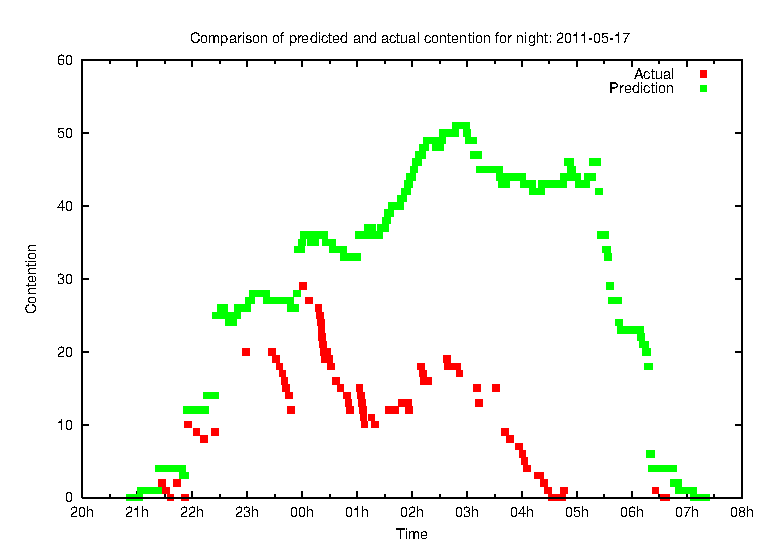
\includegraphics[scale=0.8, angle=0]{figures/contention_2011-05-17.eps}
  \end{center}
  \caption[ Comparison of predicted and actual contention on a typical night.]
   {Comparison of predicted ($C_C$) and actual contention ($C_A$) on a typical night. $C_A$ follows $C_C$ at the start of night and tracks any upward trends asnew groups become observable but over the course of the night $C_A$ slowly drops off. As runs of observations occur, $C_A$ is seen to follow a descending staircase pattern as the pool of observations is depleted.}
  \label{fig:contention_plot}
\end{figure}


\subsubsection{Demand profile $C_d$}
\notation{name={$C_D$},description={Demand profile},sort={C}} A given group will potentially have multiple observing windows when it should be attempted. During any given window the group can be considered to have a demand $C_D$ on the time within that window. E.g. if the group $g$ has an (estimated) execution time $X(g)$ \notation{name={$X(g)$},description={Execution time of a group},sort={X}}and its window of opportunity is $\phi(g)$ \footnote[1]{this is the window during which it may legally start, it may run on over the end of the window as this is taken account of in determining whether the group could be executed} then the group's demand over that window is $C_D=X/(X+\phi)$. If we add up the demand contributions of all the groups which are enabled at any given time we should have a measure of how much demand is placed on that instant. If this aggregate demand exceeds unity then it is likely that some of the groups will not be observed i.e. the requirement for time is greater than the time available. 

There are several refinements that can be made on this estimate. Firstly we can work out the numerator fairly easily. It can usually be considered constant and known. The denominator is more of a problem. Firstly working out the window of opportunity from the group's time constraint window is straightforward, however this window may extend from just a few minutes upto several days or even weeks. In the later case the group's target(s) may rise and set several times and the various implicit timing constraints may be broken on several occasions. The lunar distance constraint will impose a varying overlap with the target visibility windows. Any solar elevation constraint will vary the length of available night depending on the time of year. If we consider each of the calculable constraints then we can work out the actual amount of time (within the window) that the group can actually be observed. This gives us a revised (increased) estimate for the group's individual demand for those times within the new sub-windows. 

Going on another stage we might consider those constraints which cannot be worked out in advance. A group may have a minimum seeing constraint, however, we cannot tell what the seeing will be like at any future time though we may be able to estimate the likeliness of attaining the group's minimum level. Likewise we can obtain estimates of extinction (perhaps including seasonal variation). We should in addition consider the probability that the selected time is even available for observing. Weather and technical downtime mean that a certain fraction of time is lost. A crude climatological estimate might just give the average probability of bad weather (averaged over long periods), we shalllater see (Sect.~\ref{ss:weather_anal}) that this is around 20\%. We might also have more accurate seasonal-adjusted climatological information. If we could predict for some time ahead based on current and recently collected weather data then we should have an even better demand estimate. 

Formally, let $X(g)$ represent the \emph{estimated} execution time of a group $g$ and $U(g,t)$ the remaining useful time left for that group at time $t$, then the partial demand of $g$ at time $t$ is defined as:-

%\begin{equation}
%d(g,t) = X(g)/(X(g) + U(g,t)) 
%\end{equation}
%%\begin{equation}
%U(g,t) = \tau(w^*_i) \cap [t,\infty] \cap N(t) \cap M(g) \cap V(g))
%\end{equation}

\begin{align}
\label{eq:demand}
  d(g,t) &= \frac{X(g)}{X(g) + U(g,t)} \\
  U(g,t) &= W^*(g,t) \cap N(t) \cap M(g) \cap V(g))
\end{align}


where $W^*(g,t)$ is the set of remaining sub-windows (running forward from t) for the current execution of the group, $V(g)$ is the set of visibility windows for $g$'s targets from $t$ onwards, $M(g)$ is the set of windows satisfying $g$'s observing constraints, $N(t)$ the set of nights from $t$ onwards.

It should be clear from this discussion that calculation of demand is a computationally costly exercise. In general it proves convenient to restrict the look-ahead to the current night giving a slightly higher estimate than would otherwise be made.

%Some stuff on seeing/extinction stats. More on weather/technical downtime.

%If a group $g$ is to execute at some future time $t$ we need to know that the weather will be good at that time and that it will remain good for at least $X(g)$. From the weather stats:- 

%\begin{equation}
%P_{exec}=P_{good}(t) \dot \int_{t=X(g)}^{t=\infty}{\rho(t)dt}
%\end{equation}

%where $\rho(t)$ represents the distribution of lengths of continuous \emph{good} weather runs.

\subsubsection{Load $C_l$}
\label{sect:metric_load}
\notation{name={$C_L$},description={Schedule load},sort={C}} Load is a fairly simple metric which describes the ratio of executable time in a given observing night to the length of the night (or astronomical night). Simple load is calculated using the sum of execution times for each executable window of each group that can be executed during the night. It includes all windows of all groups whether they \emph{must} be executed that night or not. An urgency weighted load $C_{ul}$ \notation{name={$C_{UL}$},description={Urgency weighted load},sort={C}} can also be calculated which weights each execution time by the reciprocal of the number of remaining nights in which the window could be observed. Critical load $C_{cl}$ \notation{name={$C_{CL}$},description={Critical load},sort={C}}is a pruned version of the normal load where only groups which {\bf must} be executed that particular night are included. Priority weighted load $C_{pl}$ is calculated by taking into account all of a group's windows which should be executed on a given observing night then weighting by the priority of the group whose window it is.

%TODO Include cc,ca cd profiles for a single night from collected data. these are refd from 2nd section/para??

\subsection{Schedule quality metrics (SQM)}
\label{sect:sqms}
%These are the metrics used to compare the results of using different schedulers or scheduling policies on a given scheduling problem. These are needed to determine which scheduler performs best. Needless to say this is the most difficult problem for several reasons.
One aspect of the planning and scheduling process is \emph{to maximize the profitability of the enterprise} \citep{miyashita96distributed}. The enterprise is the telescope or the group which runs it. Profit refers here to some accumulated reward the \emph{owners} expect to get from providing the facility. This could be money, in terms of grants recieved for the continued provision and expansion of the service or could refer to some general sort of kudos within the scientific community resulting from the perception of the current and potential users that it is a novel and useful facility.

%\begin{itemize}
%\item The metric used in the selection heuristic cannot be used for the simple reason that these may be what distinguishes one scheduler from another - clearly if we use a metric $m_1$ for scheduler \emph{S\_1} and metric $m_2$ for scheduler \emph{S\_2} then measuring the performance of both schedulers using $m_1$ would naturally find that \emph{S\_1} was the better scheduler. Likewise using $m_2$ to compare the results would reveal \emph{S\_2} as the better scheduler. We therefore need a more generic metric which is ideally {\bf NOT} involved in the selection process.
%\item What was that other one ?
%\end{itemize}

%This turns out to be particularly difficult. In the common scheduling literature there are many generic metrics used, however these all suffer from the problem that they are tuned for the generic job-shop scheduling problem in which a number of identical jobs with specified due dates have to be processed. Typical metrics include:-

%\begin{itemize}
%\item Slack - the amount of time where no job is in progress.
%\item Tardiness - total lateness for jobs executed.
%\item Throughput - total no of jobs through the system.
%\item other
%\end{itemize}

%Can we use any of these ? The problem is that the OGs generally have a due dates which cannot be exceded - if they are late the data is of less or no use. We are not neccessarily bothered about throughput so much as the quality of the results. 

%we might be able to use some of this however with suitable weighting e.g. a late high priority job is worse than a late low priority job (but by how much?). 

%We can seperate out various forms of utility measure (NOTE these are discussed elsewhere but not in correct place)

%User based (needs simple Phase2 specification or QOS metrics)
%Enterprise based - includes scientific priorities, distribution of time between proposals

The utility or reward can be looked at from 2 (sometimes conflicting) points of view. We need to be able to measure a quantifiable reward resulting from performing the most scientifically useful or \emph{in-vogue} research whilst at the same time meeting the various users' preferences. %We need some way for the scheduler to select observations which will generate the highest cumulative reward and on a consistent basis, i.e. we need metrics to classify groups of potentially schedulable groups over time. 


%It does not want to sit about doing nothing just so it can wait for a high value observation with a small window of opportunity %(graph showing a schedule snippet with 2 low value but long groups and little idle time and 2 high value (scientific priority) but short groups with a heap of idle time) if we consider the figure the low value groups give a low sum score $\sum V_i$ for the night if we just add their individual utilities whereas the high value groups give a high sum score. On the other hand if we do an integral (int V(t)) we get a better score for the low value groups. 

. %These can arise for several reasons:-
%There may be an idle gap between groups due to the specific enablement windows, during the execution of a group we can distinguish useful and wasted time - useful time is basically exposing (and to some extend readout which we cannot avoid), wasted time includes slewing, selection and configuraton of instruments, acquisition by autoguider, settling time, and the scheduling time itself. 
\begin{itemize}
\item \emph{Enterprise utility} $V_e(g,t)$ \notation{name={$V_e(g,t)$},description={Enterprise utility for executing group $g$ at time $t$},sort={V}} represents the reward to the telescope or facility. Ideally the enterprise wants to do (scientifically) valuable work and as much of it as possible. Some of the factors which might influence the enterprise view include:-
\begin{itemize}
\item Proposals have already been vetted and prioritized on the basis of scientific importance by the allocation committees so this provides a useful measure.
\item The enterprise does not want to waste high quality time making observations which could be performed in poorer conditions so a measure of matching conditions to minimum requirements.
\item The enterprise may be more inclined to reach particular stages of completion for certain (high valued) projects over other lower valued projects.
\item Conversely there may be a requirement to share out general observing time (and time under various conditions) between projects or sponsoring TAGs in previously negotiated proportions.
\item We may want to factor in any periods of idle time caused by waiting for specific groups to become enabled as a penalty/cost term.
\end{itemize}

\item \emph{User utility}  $V_u(g,t)$ \notation{name={$V_u(g,t)$},description={User preference utility for executing group $g$ at time $t$},sort={V}} represents the reward to the individual users in respect of their own preference metrics. From a user's point of view, the ideal schedule is probably one in which all of that particular user's feasible observations would be done at their optimum times irrespective of any other user's requirements. Of course we cant always work out these optimal times. We can work out when the target will be best placed, e.g. at its highest elevation in the current window whilst bearing in mind that the window may extend over several nights, but we cannot say what the conditions will be like at that time. The telescope may be out of action due to weather or the seeing could be very poor. 

The individual users will have some preferences on when and under what conditions their observations are performed. They are able to specify the minimum conditions and the timing intervals and various constraints on their observations but these preferences are not ordered in any way - e.g. one user might prefer that their observations are done at low airmass and be less concerned with regularity whilst another user may be less concerned with airmass but more so with regularity. The simple constraints do not allow these preferences to be taken into account, instead a generic preference weighting is applied by the scoring and selection models so that all observations are treated as if the users had the same preference weighting. 

The user's preferences metric could include factors such as how close to centre of time window, how good the airmass, how well conditions are/will be matched. Each group could have a set of user-specified weights for these as they would have their own preferences as to which are more important and the relative importance of particular attribute values. Factors which we might include in $V_u(g,t)$ include:-
\begin{itemize}
\item airmass 
\item sky brightness
\item seeing matching
\item window position
\item data profile tracking
\end{itemize}

\end{itemize}


%We can also work out the utility $u_i(t)$ for a group over the night, this will have some maximum value $u^*_i(t)$ in any given night - this is the optimum time to do the group so we could work out $u_i(t)/u^*_i(t)$ so the utilities are normalized - do we need to do that?

With these points in mind, a first attempt at an overall utility measure for a night might look something like Eq.~\ref{eq:utility}.
\begin{equation}
\label{eq:utility}
V_{night} = \mathop{\sum}_{g_j \in G(S_i)} ((w_{u}*V_{u}(g_j,t_j) + w_{e}*V_{e}(g_j,t_j))*\tau_j) 
\end{equation} 
where $w_{u}$ is the weighting for user's preference satisfaction, $V_{u}(g_j)$ is the value the user assigns to the performing of his observation at the selected time, $w_{e}$ is the weighting for enterprise value, $V_{e}(g_j)$ is the value of scientific priority and other enterprise measures assigned to the chosen observationsand $\tau_j$ is the execution time of the $j^{th}$ group.

This metric adds in the contribution from enterprise and user-preference matching but if all users are free to specify their own weightings this might be thought to cause problems with comparison. E.g. If user $A$ assigns preferences so his observations are always good i.e. he has no preference and user $B$ chooses his preferences so his observations are best at $t_B$, user $A$ will get a better score contribution most of the time. However it should be noted that we are not suggesting use of this measure as a selection metric to select $A$ over $B$ but to merely as a measure of the quality of the schedule for the night


%\subsubsection{Potential utility measure} Work out the best utility that can be achieved during the night (PU) (i.e. assume we can do all the groups that could be done and do them at the best possible times) - this is after all the ultimate aim of the scheduler ! Work out the actual utility scored by the scheduler that night - the Efficiency (E) is then the ratio. May need to scale - after all if oversubscribed we could never do it all anyway try load scaling 1/L (load defined as aggregate (average) demand) or maybe better as \emph{sum of execution times of all groups that can and {\bf should} be executed tonight}. Could also try rank-scaling top(n) such that $\sum{x_i} < \tau(n)$ - I cant quite recall what I meant by that at the moment.


\subsection{Primitive utility measures}
Needless to say, choosing the relevant enterprise and user metrics and deciding how these should be weighted is no easy matter and depends on too many factors to come up with a definitive answer which would be of use in the ensuing experiments. Consequently we are forced to find some simpler/more primitive metrics to use. 

\begin{itemize}
\item Height metric $Q_H$ measures the difference between the optimum time for performing a group based on its height to transit height ratio during the night and its actual selected time of execution. By adding these offsets for all selected groups we get a measure of badness. Ideally all groups would be executed at their highest point (in the current feasibility window) so this measure should be close to zero. 

\item Optimal Height metric $Q_{OH}$ \notation{name={$Q_{OH}$},description={Optimal height quality metric},sort={Q}} measures how close to the \emph{optimum} height the group is observed in its execution window. 

The optimum height is basically the highest elevation attained by the group during the feasible observation window - in a given window this may be at the end (rising target), start (setting target) or somewhere in the middle of the observing window (transiting target). 

There is however a non-linear relationship between elevation and airmass such that for targets which do not rise particularly high the difference in image quality between worst and best case elevation may be high over a relatively small elevation difference whereas for high rising targets the difference in airmass and hence image quality between best and worst case elevations will be small for the same elevation difference .

Consequently it may be better to measure the ratio of execution-time airmass $a_{actual}$ to best achievable airmass $a_{opt}$ as an Optimal Airmass metric $Q_{OA}$.\notation{name={$Q_{OA}$},description={Optimal airmass quality metric},sort={Q}} 

Additionally, the \emph{benefit} (image quality advantage) of one airmass over another may itself be non-linear and this is what we should really be measuring. $Q_{BA}$ \notation{name={$Q_{BA}$},description={Airmass benifit quality metric},sort={Q}} measures the ratio of some decreasing benefit function $b(a)$ of airmass $a$ at optimal airmass and actual execution-time airmass. A simple option for $b(a)$ would be to use the known correction \cite{sarazin90eso} of image FWHM or seeing $s$ for airmass relative to \emph{ideal} seeing at elevation $90^\circ$, $s(a)=s_{90}a^{0.6}$ with $s_{90}$ indicating the image FWHM at $z=0,a=1$ and assuming image quality is judged purely (and linearly) on FWHM. It should be noted that this correction depends also on observation wavelength $\lambda$. 

\begin{equation}
Q_{OA} = \frac{1}{L_N}\sum_{g \in S}{\frac{a_{opt}}{a_{actual}}}
\end{equation}
where $a = \sec{z}$ is the airmass of group's target at zenith distance $z$.

\begin{equation}
Q_{BA} = \frac{1}{L_N}\sum_{g \in S}{\frac{b(a_{actual})}{b(a_{opt})}}
\end{equation}
where $b(a)$ represents the benefit (image quality advantage) for airmass $a$.

\item Monitor window metric $Q_{MW}$ \notation{name={$Q_{MW}$},description={Monitor Window quality metric},sort={Q}} measures the difference between the optimum time (relative to the centre of a monitoring window) for performing a group based on the known monitor window and its actual selected execution time. By adding these up we get a measure of badness in terms of offsets from the optimal time. Ideally all groups would be executed at the centre of the monitor window. There are some implications in respect of non-monitor groups. How do we select the centre of the window ? What if the window centre is not actually feasible, how is this taken into account ? In practice these difficulties led to this metric not being used for the experiments but it might be used in future if these problems could be satisfactorily sorted out.

\item Priority metric $Q_{PX}$ \notation{name={$Q_{PX}$},description={Execution Priority quality metric},sort={Q}} measures the total priority score achieved i.e  sums up the priorites of the groups selected. As Proposals have already been vetted and prioritized by the allocation committees, this provides a useful source of information.  The final value can be normalized by dividing by the length of night (or astro-night) or perhaps better by using the priority weighted load $C_{pl}$ (Sect.~\ref{sect:metric_load}) as this also gives an indication of the degree of \emph{missed opportunity}.
\begin{equation}
Q_{PX} = \frac{1}{L_N}\sum_{g \in S}{X(g,t)p(g)}
\end{equation}
where $p(g)$ is the priority value for group $g$ and $X(g,t)$ is the estimated execution time for group $g$ at execution instant $t$.

\item Target demand metric $Q_{TD}$ \notation{name={$Q_{TD}$},description={Target Demand quality metric},sort={Q}} measures how \emph{urgent} the selected groups are with reference to the night's demand profile $C_d$.
\begin{equation}
Q_{TD} = \frac{1}{L_N}\sum_{g \in S}{f_D(g,t)}
\end{equation}
where $f_D(g,t)$ represents the value of the demand (Eq.~\ref{eq:demand}) for group $g$ at execution instant $t$. 

%\item Night windows count metric $Q_{NW}$ is an attempt to guage the number of nights in which a group could have been selected - it is effectively a count of the number of subwindows in which a group could be executed - a high value indicates that the scheduler is picking groups which dont have to be selected on that night, conversely a low value indicate a scheduler which is picking groups for which execution on the night is more critical. 

\item Execution time metric $Q_{XT}$ \notation{name={$Q_{XT}$},description={Execution Time quality metric},sort={Q}} is a measure of the amount of the night during which groups are actively being observed. A low value is effectively an indication of \emph{slack time}.
\begin{equation}
Q_{XT} = \frac{1}{L_N}\sum_{g \in S}{X(g,t)}
\end{equation}
where $X(g,t$) is the estimated execution time for group $g$ at execution instant $t$.

\item Remaining nights metric $Q_{RN}$ \notation{name={$Q_{RN}$},description={Remaining Nights quality metric},sort={Q}} counts a decreasing function (for convenience 1/n) of the \emph{number of nights remaining} $n$ for any groups in the observability window $\Phi(g,t)$ at the time of selection/execution. It effectively measures how \emph{urgent} the window was in terms of the number of future chances of executing 
the group other than tonight. e.g. If a group could be executed tonight or on 3 future nights this yields a value for RN of 4 and thus 1/4 as its urgency.
\begin{equation}
Q_{RN} = \sum_{g \in S}{\frac{1}{R(g,t,\Phi(g,t))}}
\end{equation}
where $R(g,t,\phi)$ counts the number of remaining nights for a feasiblity window $\phi(g,t)$ of group $g$ at execution instant $t$ - i.e. it counts the number of feasible future sub-intervals of $\Phi$ with maximum of 1 per night.

\item Project completion $Q_{PC}$ \notation{name={$Q_{PC}$},description={Project Completion quality metric},sort={Q}}has been suggested as a metric for comparing scheduling policies or schedules generated by different schedulers ( XXX SPIE paper from?? and UKIRT paper). I suggest that this is not always a good metric - a project which relies on gathering data over an extended period and for which the length of data gathering, periodicity of gathering are more important would not be well served by completing the program in the fastest time. For such programs we should be more concerned with producing data at a rate which tracks the expected production rate of data. In addition we would like to generate the best quality of data or at least data of a quality which meets or exceeds the programs stated requirements - e.g. we select an observation to be done in seeing which is as good or better than required, at low airmass and any other factors which could contribute to its quality. When considering flexibly timed groups it should be noted that these receive all of their data in a single chunk. It is therefore not feasible to \emph{track} these. Finally, we do not always have enough information available early in a semester. Some users put all of their groups in at the start, some feed them in over the semester so we cannot in general know how complete projects are at any time.

%Note: Global optimization is what we want but local optimizer may be sub-optimal e.g. of Despatch compared to (short) lookahead. Example when groups have finite and variable enablement intervals EI (use proper symbol). Should we be trying to optimize in terms of when is the best time I can do this group rather than what is the best group to do now. \emph{Description of an example with g1 long EI g2 with short EI but v.hi score. g1 selected but wipes g2's EI. Could have picked g3 with short exec then g2 - overall score is higher and still do g1 later with good score - include a diagram showing the score profiles for the groups}.

\item Condition matching metrics $Q_{xM}$ \notation{name={$Q_{SM}$},description={Seeing condition Matching quality metric},sort={Q}} \notation{name={$Q_{LM}$},description={Lunar condition Matching quality metric},sort={Q}} assigns a measure to how close the actual conditions (x) are to those requested in a group's observing constraints as being the minimum acceptable. This metric is designed to prevent groups with \emph{low quality} requirements using up time which might be classified as \emph{high quality}. In practice the atmospheric seeing (S) and lunar darkness (L) are used for this purpose.

\item Yield tracking metric $Q_{YT}$ \notation{name={$Q_{YT}$},description={Yield Tracking quality metric},sort={Q}}measures the yield of a group of observations. Put simply, this is the ratio of the quantity of data taken (observations) at a given time relative to the quantity that would have been taken upto that time given that the group was observed at each occasion when it could technically been observed. Calculation of this metric presents some difficulties. In the case of groups with \emph{minimum interval} timing constraints it is not possible to give an actual figure for the potential number of observations made as the constraint does not specifiy a maximum interval. For practical purposes this is taken to be twice the value of the minimum interval. In the case of groups with \emph{flexible} timing constraints, the potential yield is calculated as a fraction of the time between activation and expiry even though there can only be one occasion when the observations are ever made. 

\item Resource allocation/usage metrics $Q_{Ax}$ for various resources $x$ against target values. Thse would probably be long term metrics, valid over periods of order semester or year, a metric currently in use by the operations team is the TAG assigned Minimum Use Fraction (MUF) \glossary{name={MUF},description={Minimum Use Fraction - a TAG assigned target for program completion},sort={M}}.

\item Multiple combined metrics such as $Q_{OA \cdot PX}$ would allow pairs (or larger tuples) of metrics to be combined as would linear combinations such as $w_{oa}Q_{OA}+w_{px}Q_{PX}$. \notation{name={$w_{x}$},description={weighting factor for metric $x$},sort={w}}

\end{itemize}

%\begin{figure}[h]
%\subfigure[Comparison of models for determining airmass image quality advantage ($b(z)$)]{
%    \label{fig:baz_plot}
%    \includegraphics[scale=0.25, angle=-90]{figures/baz_plot.eps}
%  } 
%\caption{Various metric models}
%\end{figure}

\subsection{Matching metrics to scheduling and planning horizons}
\label{sect:matchmetrics}
As can be seen the various $Q$ metrics already discussed cover very different time-scales. It is perhaps appropriate then to see how these might be applied in reality to different scales of planning and scheduling. Table.~\ref{tab:planning_metrics} is an attempt to match the various $Q$ metrics to the different planning or scheduling horizons discussed in Sect.~\ref{sect:pandstimescales}

\begin{table}[htbp]
 \begin{center}
  \begin{tabular} {|l|l|p{7cm}|}
    \hline
    Planning Level &  Period              &      Metrics\\
    \hline
    SP (strategic) &  1 semester or more  & YT (yield track), PC (program completion).\\
    \hline
    TP (tactical)  &  1 week - 1 month    & PC (program completion), Ax (resource sharing).\\
    \hline
    MP (mission)   &  1 night             & TD (target demand), RN (remaining nights).\\
    \hline
    S (sched)      &  1 horizon           & OH (optimal height), P (group priority), LM (lunar match), SM (seeing match).\\
    \hline
  \end{tabular}
  \label{tab:planning_metrics}
  \caption[Assignment of $Q$ metrics to hierarchic planning levels.]{Possible assignement of $Q$ metrics to appropriate layers of the planning and scheduling hierarchy. As the horizon increases up the hierarchy, the metrics used are likely to be calculated over longer periods of time with possibly large night to night variation. At the scheduling end of the hierarchy, metrics are calculated on a per-group execution basis.}
 \end{center}
\end{table}

\subsection{Conclusions}
I have discussed two main types of metric. Quality (or Q) metrics measure the results of scheduling. A realistic $Q$ metric would include both user and enterprise requirements, however for simplicity and because there is currently no way within the Phase 2 system to include user requirements a set of primitive measures have been defined. Complexity (or C) metrics measure the difficulty or \emph{density} of a scheduling problem and are an attempt to capture the highly complex multi-dimensional structure of the Phase 2 information in a few simple parameters. The measures suggested are relatively easy to compute and give a flavour of the problem.


%\subsection{Discussion}
%Discussion of some points not covered already. Open questions. MOVE THESE TO C/FW OR ELSEWHERE

%\begin{itemize}

%\item It had originally been intended to use these to minimise the sum of differences between the actual and optimal execution times - a good schedule then would be one in which the metric gave a low or best case zero result. A problem with this is that it is possible to achieve such a score by simply ommitting to perform observations - this is reminiscent of the train performance metrics used to measure the efficiency of privatized railway companies. If a train is running very late - simply cancelling the train removes it from the lateness statistics adding to the misery of the waiting passengers - its little comfort that the next train is on time if they have had to wait an hour for it !. Consequently these metrics must be scaled to give a high score when the measured variable is at maximum, lower measures when the time is poorly met and zero (or even negative) scores when the observation is not attempted. A schedule which simply avoids potential observations would then score badly. 

%\item The best schedule for a given night is the one where every {\bf critical} group is executed at its best time (ie when its overall utility is highest) and where the remaining groups (if any) are selected ``appropriately''. To determine what this actually is requires to test every feasible combination of critical group (and others) to see what could be achieved. This may then need to be done for different environmental assumptions for the night ahead. The remaining (non-critical) groups should probably be selected to miximize profit over a period (rather than for that specific night). All this makes no assumption about additional groups added via ODB mutation.


%\item Need to look at longer term aims (i.e. those that would be introduced by a tactical/strategic planner) - these include things like- fairness between users/TAGs, distribution of environmental conditions, darkness, regularity of data product etc. It may not be neccessary however to worry about these from the scheduler's pov as it is by neccessity working on a shorter timescale - these higher order entities can force appropriate changes in the scheduler's behaviour by altering the control parameters (and metrics) used by the scheduler to satisfy their longer term aims.  
 

%\item User preference on when to be done should be taken into account - rather than do X now just because it has highest score in a global sense, do Y because its best time to be done is now, whereas as X would prefer to be done later when its score is higher - (Granzer includes time profiles in \cite{granzer03stella})

%\item Useful link to Bresina's thesis chapt3 has notes on contention and demand profiles - these equate roughly to my aggregate demand profiles and tracking metric http://ic-www.arc.nasa.gov/ic/projects/xfr/sampling/thesis/index.html.

%\item Given a utility measure $F(g,t)$ which describes the value of performing group $g$ at time $t$, the potential utility metric is the sum of the individual values of $F(g,t^*)$ for each group execution window on the night ${n}$ containing $t$ at the time $t^*$ which maximizes  $F(g,t)$ for that group. In other words it is the total utility which could be achieved that night if all feasible groups were executed at their optimum time. In reality it may not actually be possible to achieve this as several groups could be optimal at the same time or overlapping times. Also if the total execution time potential for the night exceeds the available night-time hours it ill not be possible even without overlaps. The metric can of course be scaled by a factor $\tau({n})/\sum_{g \in G{(n)}}{X(g)}$. The performance metric then becomes $E_{{S}}/E_{potential}$  where $E_{{S}} = \sum_{g \in {S}(g)}{F(g,t^*)} $. 


%\subsubsection{More about contention to squeeze into discussion above}
%There is a need to measure the contention for time among the groups enabled on a nightly basis, it would be useful to be able to do this on a fine granularity - e.g. minute by minute. First we must decide what we mean by contention. My definition is the degree of demand by all enabled groups for a given slice of time - put simply, if a group needs 10 minutes to execute and there is a 30 minute window of opportunity in which it can start, then its demand for the whole of this window is 10/30. If there are other groups which also have some demand for all or part of the window then they will contribute appropriate amounts to the total demand for the window to those fractions of the window during which they are enabled, the total (aggregate) demand at a given time then is the sum of all the partial demands from each group whose enablement interval includes that time. Put more formally:

%$T(t) = \sum_{g : w \cap t} { \frac{t_x(g)}{w_e(g)} }$ 

%TODO this needs writing properly 
%TODO also need some formal definitions for w/W/tx etc and where they are got from.

%How then do we calculate this ? The numerator is the easiest - define the components of this along with any uncertainty terms and consideration of parallelism - this is obtained from the ExecModel. First we must decide what we mean by enablement window. Each group has by reason of its TimingConstraint a set of one or more windows in which it is intended to observe (execute) the group (also called a visit in some systems - need a distinct word), in the case of a Flex group this is a single window [ts,te]. For a periodic monitoring group there will be a series of windows $w_i = [ts+i*p-w/2, ts+i*p+w/2]$ such that the last window stops around $t_e$. As a first approximation then the denominator can just be considered to be the size of any window which includes t - (Note no group should by definition of the various timing constraint classes have more than one window corresponding to any given time). Because we have an optical telescope and observe only at night, we can restrict the actual time available to a group for the execution of its observing window to the intersection of the window with the night which includes t. So $t_avail = W \cap N(t)$, thus incresasing the contention contribution. A number of additional approximations will continue to pare this denominator down so we can expect the first approximation to be significantly low. We should note some points here. I have so far assumed implicitly that the group's window of opportunity W is less than the duration of a single night, this will often not be the case, i.e. many group windows extend over serveral days (and nights) and in some case, especially long activation flexible groups may run for weeks or months, so the actual $t_avail$ in these cases should really be represented by W intersect {N} where N is the set of all the future nights for which the group is available. We cannot stop here, just because it is night does not mean we can make the observation, the target will not neccessarily be visible, either above the geographical horizon or any operational horizon of the telescope, so we can further reduce the available time by considering only the part of the night(s) where the target(s) are visible $t_avail = W \cap N \cap V$. Each group has associated with it a number of observing constraints - some of these represent implicit additional time constraints, namely those which can be calculated in advance. An example would be the lunar distance constraint - the observations in the group cannot be made if the moon is less than some given distance from the observation's target. If we add these into the mix we get an extra reduction in the available time for the group to execute - bearing in mind that these calculations must be performed for all future nights which intersect the group's window containing t. We have done all that is possible with the certain knowledge of the observing environment, there remain however a number of uncertainties - we have not considered either those observing constraints which refer to environmental conditions which cannot be predicted in advance with any certainty, e.g. the group's available window will most likely be reduced further if the seeing is worse than the maximum specified in the seeing constraint, similar things may be said concerning other unpredictable elements. (which). We can further reduce the available window if we can predict when the telescope will be unable to observe due to poor weather, mechanical or technical faults, engineering and other downtime. If we can at least obtain some statistical values for these, which may contain seasonal or other variations (e.g. weather downtime, or seeing distribution dependant on time of year) or we can predict sky and weather conditions for the night ahead with some accuracy (this will help for short period monitors) then we can get produce weighted contention profiles.

%\item The scheduler is basically answering the question - \emph{What is the best thing I can do now from those things available ?} rather than the possibly more useful from the users' pov \emph{When are the best times these available observation could be done ?}. If we can allow the user's own preference weighting to be taken into account then we will have a more user-centred view of the schedule. How can we do this? There are several options.

%\item We can always consider the scheduling process to be a competition between users (groups of observations) for particular time slots. After the scheduling process is completed by whatever means it represents the best allocation of times to groups. In reality we do not expect to be able to extract a full schedule to cover say a whole night due to the dynamically changing environment, however we do still want to get the best observations at each time slot whether by selecting individual groups at the time (despatching) or selections of groups over a horizon during which the conditions (and goals) are predicted to remain reasonably stable. 

%An obvious direction to follow is the auction path. We could allow the users, in reality some per-proposal delegate (agent) acting on the user's behalf to bid for time available slots as they became available. One would image the SE deciding the current time horizon based on environmental stability predictions, perhaps predicting goal evolution (P2DB evolution) on the basis of past behaviour and using knowledge of RCS future commitments (e.g. RTI or calibration time), then advertising the time slot(s) available to interested delegates. The delegates would examine their groups' requirements and decide whether to bid for any slots. More advanced (and $O^n$ more difficult) - combinatorial auctions.

%\item  Scheduler using PCMs as feedback. This would introduce a feedback effect which would make the whole exercise rather more difficult as the degree of feedback ought first to be determined and taken into account in making any assessment of complexity.

%\end{itemize}


% ENVIRONMENT/DB/VOL CHARACTER
\section{Characterization of operating environment}
\label{sect:character}

I have already stated (Sect.~\ref{sect:intro_background}) that the telescope operates in an \emph{uncertain environment}. In order to be able to make planning and scheduling decisions over the range of timescales outlined in Sect.~\ref{sect:pandstimescales} it will be neccessary to determine what constitute the components of this environment, to ascertain the range and variation of these components and to examine how such variation might impact on both the ability to schedule and the potential reward available. 
 
Though many of these processes are naturally unpredictable, it would be very useful to be able to at least have some way to determine the likeliness of these conditions occurring. If we could determine that the telescope would not be able to observe tomorrow, then we could ensure that an important observation was made tonight even though the potential reward might be better tomorrow. Conversely if we knew for certain that the telescope would be available tomorrow then we might make a low priority but urgent observation tonight and do the less urgent but higher priority observation tomorrow.

\subsection{Environment Components}
\label{sect:env_components}
The operating environment characteristics can usefully be broken down into the following components. Each of these can affect the operations of planning and scheduling in particular ways.

\begin{itemize}

\item {\bf Technical faults}. Mechanical, electrical, software and communications systems faults can leave the telescope unable to operate or may severely impair operational effectiveness. In some cases the telescope may be deliberately shutdown to permit preventative maintainance.

\item {\bf Bad weather}. Rain, high humidity, strong or gusting wind and calima (Saharan dust) can force the shutdown of the telescope systems to prevent damage to delicate instrument, optical and electrical hardware. The presence of ice prevents the dome from opening due to likely damage to the rams. Under any of these conditions, no observing is feasible. 

%  \begin{itemize}
%    \item rain can lead to ingress of water into delicate instrument, optical and electrical hardware.
%    \item high humidity may cause condensation on optical and electrical hardware.
%    \item high or gusting winds may damage the mechanical structure and tracking performance may be effected by wind-shake.
%    \item calima (Saharan dust) is a problem during the summer months causes damage to optical and mechanical systems.
%  \end{itemize}

\item {\bf Poor Sky conditions}. Do not pose problems for infrastructure but can severely disrupt the ability to perfom useful observations. Extremly bad seeing, high extinction or high background sky-brightness lead to the requirement for longer exposures to achieve required signal-to-noise ratios (SNR\glossary{name={SNR},description={Signal to Noise ratio}}). In addition the pool of feasible observations is reduced as the conditions worsen leading to lower contention (easier scheduling task) but at the same time to reduced potential rewards.

\item {\bf Phase 2 population}. The actual content of the Phase 2 ODB affects how scheduling decisions are made. The distribution of the large number of its characteristics determines both the contention at any time and the potential rewards available. External software agents and users can modify the content of the Phase2 ODB at any time. Where these modifications occur during the night it seems reasonable to assume they will have some effect on the character and potential profitability of schedules which might be generated and introduce extra complexity into the scheduling operation.

\end{itemize}
  
\subsection{Technical faults}
The telescope is a complex system made up from numerous components. Though it has many inbuilt recovery mechanisms there are times when the overall system is unable to function without direct human intervention. Problems may occur with any of these systems:-

\begin{description}
\item [Mechanical] Physical problems with components such as:- main axes, focus drive, enclosure hydraulics, science fold deployment and instrument components such as filter-wheels and slides.

\item [Electrical] Power supplies to the site are occasionally disrupted though sometimes this information is available in advance.

\item [Network] Problems due to internal (inter-system) communications breakdown. These may be as simple as a wire dropping out, a software configuration problem or due to heavy network loading - typically a symptom of some other underlying problem. 

\item [Software] Low and high level systems can cause problems. These are highly complex systems and thus difficult to test thoroughly even with use of a simulated environment so problems can occur, particularly during upgrades. 

\end{description}

Several (7) years of knowledge gained from operating the telescope allow these errors to be classified into a few basic categories with differing timescales from inception to solution.

\begin{description}
\item [major catastrophy] These are problems which suddenly manifest themselves one night causing major downtime. Often these are due to mechanical breakdown of a component which requires a site visit to repair. The time involved can potentially be days if spares are not immediately available and no workround can be arranged. Where serious software failures occur, these are generally fixed within a day by a concentrated effort.

\item [occasional glitch] These are problems due to either non-terminal failure of a mechanical component which is too expensive to justify replacing or more often a known but difficult to repair software problem. The frequency of occurance and degree of impairment will tend to determine how much effort is employed on the solution.

\item [sporadic bug] Sometimes the problem is very difficult to identify and needs to occur many times before enough information is gathered to identify the cause. 

\item [shakedown] Effectively time required for new mechanical components or software deployments to bed in. Software in particular may be tested on the simulator but behave differently on the actual system due to subtle timing effects or unpredicted coincident situations.
\end{description}


\subsubsection{Source of data}
The main source for this information is the nightly logs kept by telescope operations staff\footnote{Obtainable from: http://telescope.livjm.ac.uk/News/Reports/}. These consist of the number of hours of technical downtime, weather downtime and actual observing hours per night. This information is assessed by a combination of examining system logs and from personnal knowledge of the events of the previous night and so a degree of interpretation is involved. Of particular importance is the policy to assign the category \emph{weather downtime} to those periods when there was a combination of bad weather and technical problems - it is thus not possible to seperate these out. E.g. on a night where there might be 2 hours of observing mixed with 2 hours of intermittent technical problems followed by 6 hours of bad weather there is no way of telling whether the actual technical problem would have resulted in an additional period of downtime if the weather had remained good. 

Operations staff may assess early in the night that some serious technical problem is likely to affect the performance of the telescope during the night - e.g. poor image quality or tracking and decide to shutdown the telescope for the remainder of the night thus yielding an apparently high loss fraction rather than allow the automated systems to cycle between \emph{operational} and \emph{impaired} states.

Data covering a period of 30 months (919 days) for 2005, 2006 and part of 2007 was available and used to determine figures for probability of technical downtime and how this varies over the year. 

\subsubsection{Analysis}

Plots of technical downtime per night are displayed in Figs.~\ref{fig:nightly_tech2005}, \ref{fig:nightly_tech2006} and \ref{fig:nightly_tech2007}. The individual spikes represent the actual number of hours downtime on each specific night while the curved envelope reflects the variable night length over the course of the year. There does not appear to be any discernable pattern though as there is no sub-categorization of actual types of fault one cannot rule out the possibility that certain faults are more common in summer and others in winter, averaging out to a similar overall result. Basically, technical faults of some type can occur at any time.

\begin{figure}[htbp] 
\begin{center} 
 \subfigure[Technical downtime per night 2005.] {
    \includegraphics[scale=0.3, angle=-90]{figures/ecs/met_nightly_stats_tech2005.eps}   
    \label{fig:nightly_tech2005}
  }
 \subfigure[Technical downtime per night 2006.] {
    \includegraphics[scale=0.3, angle=-90]{figures/ecs/met_nightly_stats_tech2006.eps}  
    \label{fig:nightly_tech2006}
  } 
 \subfigure[Technical downtime per night 2007 (part).] {
    \includegraphics[scale=0.3, angle=-90]{figures/ecs/met_nightly_stats_tech2007.eps} 
    \label{fig:nightly_tech2007}
  }
\caption[Nightly hours plots for technical downtime for years 2005, 2006, 2007(part).]{Nightly hours plots for technical downtime for years 2005, 2006, 2007(part). Large blocks are empty due to operations policy preference for reporting bad weather downtime rather than technical when both occur simulataneously. The large empty block around February to March 2005 is due to a prolonged period of bad weather where no observing was possible.}
\end{center}
\label{fig:met_nightly_tech}
\end{figure}


Fig.~\ref{fig:tech_loss_dist} shows the distribution of fraction of night lost to technical problems, as can bee seen this is bimodal with around 72\% of nights suffering less than 5\% downtime (including those nights with zero loss). A total of 8\% of affected nights over the entire period suffered nearly 100\% downtime.  The variation of total technical downtime hours averaged by month for the available data is shown in Fig.~\ref{fig:monthly_tech_stats}. The average monthly downtime is 11.94 hrs over the period corresponding to about 0.46 hours per night.

\begin{figure}[htbp]  
  \begin{center}
    \includegraphics[scale=0.4, angle=-90]{figures/ecs/tech_loss_frac.eps}
  \end{center}
  \caption[Distribution of fraction of night lost to technical problems.]
   {Distribution of fraction of night lost to technical problems. Majority of nights have less than 5\% loss, while some 8\% suffer near 100\% downtime.}
  \label{fig:tech_loss_dist}
\end{figure}

\begin{figure}[htbp]
  \begin{center}
    \includegraphics[scale=0.4, angle=-90]{figures/ecs/monthly_tech_stats.eps}
  \end{center}   
  \caption[Monthly averaged technical downtime hours.]
{Monthly averaged technical downtime hours over the period 2005-2007 (30 months). The data only includes periods where there was no weather downtime. Average time per month lost was11.94 hrs or 0.46 hours per night}
  \label{fig:monthly_tech_stats}
\end{figure}


\subsubsection{Conclusions}
It had been hoped to look at lengths of runs of technical downtime to determine if there were any patterns - e.g. whether these occur in runs and with what distribution and frequency. Contamination of the data from weather downtime stats and the relatively small amount of data available makes this problematic. Heuristically however we might expect this to be the case. A problem might arise sporadically one night causing a degree of lost time, then maybe occurs the following night, spawning attempts by support staff to solve by software or engineering means. This may occur quickly or take several nights to correct, thereafter the problem disappears or becomes less frequent.

The diverse nature of these problems suggests that there is little chance of predicting future occurances - by their very nature they are unpredictable. The best that can realistically be achieved is to use the long term probabilities to estimate the likelihood of technical downtime over extended periods. 

Disruption to power supplies are sometimes known in advance and could be factored into medium term planning. Periods of planned maintainance are often known well in advance and could also be factored in. Prior to distribution of the Phase 2 entry system to users, both of these were implicitly taken account of by the operations team when setting up the content of the Phase 2 ODB but this information was not known explicitly by the scheduler.

\subsection{Weather}  
Weather statistics have been obtained from 3 independant sources.
\begin{itemize}
\item Data from the LT's own weather monitoring system (WMS\glossary{name={WMS},description={Weather Monitoring System}}) has been collected by embedded software for a period of 20 months/583 days at a cadence of approximately once every 32 seconds with very few gaps giving a total of 1582518 samples.% (see gap distribution histogram in Fig.~\ref{fig:gap_dist}.

\item Archived meteorological station data from various facilities at the ORM are available (\cite{sorensen02cat}) going back to 2002.

\item Observer reports of weather downtime hours per night (collated next day) for reporting on the telescope website. This data is bundled in with the technical downtime statistics and overrides these when both occur on the same night.
\end{itemize}


\subsubsection{Telescope Weather Monitoring System}%(XXX some basic info about the thing like who built it and what sensors it has).
 The Weather Monitoring System (WMS) provides feeds of various meteorological data from a weather station on site located 20m from the telescope enclosure.  Data is provided to the RCS at a cadence of around 5 seconds. The RCS filters this data and uses a set of rules (Table. \ref{tab:rcs_weather_rules}) to decide if the weather should be classified as \emph{good} in which case (all things being otherwise okay) observing may proceed, or \emph{bad} in which case observing may not proceed or if already underway should be stopped and the telescope and enclosure made safe.

Automated weather shutdowns based on WMS data are triggered by any of the following sources:-
\begin{itemize}
\item High humidity can lead to condensation on cold surfaces (mirror, electricals) and is an indicator of cloud and potential precipitation.
\item Rain causes wetting of all equipment, this has to be avoided especially on sensitive optical, electrical and hydraulic systems.
\item Moisture fraction is indicated by a digital sensor and indicates that rain or condensation is occuring or has recently occurred but not yet cleared sufficiently.
\item Cold temperatures lead to ice which can cause the enclosure portals to stick and thus put considerable strain on the motors and electrical supply if an attempt was made to open these.
\item Wind gusts  can cause damage to telescope structure and attached instruments. Moderate wind can also lead to poor tracking performance due to \emph{wind shake}.
\end{itemize}

Table \ref{tab:rcs_weather_rules} summarizes the rules in force (January 2008) for weather clear and alert triggers. A weather variable crossing its \emph{alert} level signals bad weather. In order to clear (signal good weather) the variable must pass the primary \emph{clear} level and remain below the secondary level for at least the time specified by the stability parameter. All variables must be in the \emph{clear} state for overall {\bf Good} weather. Any variable in its \emph{alert} state indicates {\bf bad} weather. Currently all rules have a 30 minute clearing stability time but this is a configurable parameter.

\begin{table}[htbp]
\begin{center}
\begin{tabular}{lllll}
\toprule
\multicolumn{5}{c}{Weather variable triggering conditions} \\
\midrule
Variable & Alert threshold & Primary clear level & Secondary clear level & Stability \\
\midrule
Humidity    &  $> 80$\%        & $< 70$\%         & $< 75$\%          & 30 min\\
Moisture    &  $> 10$\%        & $< 9$\%          & $< 9.5$\%         & 30 min\\
Wind speed  &  $> 15ms^{-1}$   & $< 12ms^{-1}$    & $< 14ms^{-1}$     & 30 min\\
Temperature &  $< 0.0^{\circ}$ & $> 0.1^{\circ}$C & $> 0.05^{\circ}$C & 30 min\\
\bottomrule
\end{tabular}
\end{center}
\caption[Definitions of alert and clear threshold levels for triggering good/bad weather conditions.]
{Definitions of alert and clear threshold levels for triggering good/bad weather conditions. A variable crossing its alert level signals bad weather. In order to clear (signal good weather) the variable must pass the primary clear level and remain below secondary level for at least the time specified by the stability parameter. All variables must be in the \emph{clear} state for overall {\bf Good} weather. Any variable in its \emph{alert} state indicates {\bf bad} weather.}
\label{tab:rcs_weather_rules}
\end{table}

The data collected consists of 1582518 samples taken at around 30 seconds cadence over a period of 30 months between 2005 and 2007. The inter-sample gap distribution indicates that there are relatively few gaps. The vast majority of the samples occur with gaps of 30 seconds or less. A small number 292 excede 5 minutes, a further 14 excede 30 minutes and 58 excede 60 minutes. The largest gap of 4.2 days occurred as a result of a site power outage
%\begin{figure}[htbp]
%  \begin{center}
%    \includegraphics[scale=0.4, angle=-90]{figures/ecs/gap_dist.eps}
%  \end{center}
%  \caption[Distribution of intersample gaps.]
%{Distribution of intersample gaps. The vast majority of the 1582518 samples occur with gaps of 30 seconds. A small number 292 excede 5 minutes, a further 14 excede 30 minutes and 58 excede 60 minutes. The largest gap of 4.2 days occurred during xxx as a result of a site power outage.}
%  \label{fig:gap_dist}
%\end{figure}


\subsubsection{Analysis of results}
\label{ss:weather_anal}
The distribution of humidity is shown in Figs.~\ref{fig:met_humidity_dist} and \ref{fig:met_humidity_cum_dist}. The distributions peaks around 15\% and average of 40\%. A very sharp secondary peak occurs around 95-100\% humidity. With the variable trigger levels (\ref{tab:rcs_weather_rules}) set to 70\% (\emph{clear}) and 80\% (\emph{alert}) these can both be seen to be well into the tail of the main distribution just before the spike. This suggests that few false alerts should occur.

\begin{figure}[htbp]
  \begin{center}
    \includegraphics[scale=0.4, angle=-90]{figures/ecs/hum.dat.eps}
  \end{center}
  \caption[Relative distribution of humidity at telescope site.]
{Distribution of atmospheric humidity at the telescope site over all samples. The distribution shows a profile with main peak around 15\% and average of 40\%. A very sharp secondary peak occurs around 95-100\% humidity. With the variable trigger levels set to 70\% good and 80\% bad these are in the tail of the normal distribution just before the spike level.}
  \label{fig:met_humidity_dist}
\end{figure}
\begin{figure}[htbp]
\begin{center}
    \includegraphics[scale=0.4, angle=-90]{figures/ecs/hum_cum.dat.eps}
\end{center} 
\caption[Cumulative distribution of humidity at telescope site.]
{Cumulative distribution of atmospheric humidity at the telescope site over all samples.}
\label{fig:met_humidity_cum_dist}
\end{figure}

% Moisture fraction
The distribution of moisture fraction is shown in Figs.~\ref{fig:met_moisture_dist} and \ref{fig:met_moisture_cum_dist}. The distribution is strongly peaked with average 0.07\%. A total of 89\% of measurements are below the alert level.

\begin{figure}[htbp]
\begin{center}
     \includegraphics[scale=0.4, angle=-90]{figures/ecs/moist.dat.eps}
\caption[Relative distribution of moisture fraction at telescope site.]
{Relative distribution of moisture fraction at telescope site. Some 89\% of nights were below the alert threshold.}
\end{center}   
\label{fig:met_moisture_dist}
\end{figure}

\begin{figure}[htbp]
\begin{center}
    \includegraphics[scale=0.4, angle=-90]{figures/ecs/moist_cum.dat.eps}
\caption[Cumulative distribution of moisture fraction at telescope site.]
{Cumulative distribution of moisture fraction at telescope site.}
\end{center} 
  \label{fig:met_moisture_cum_dist}
\end{figure}



% Wind speed
The wind speed distribution is shown in Figs.~\ref{fig:met_windspeed_dist} and \ref{fig:met_windspeed_cum_dist}. The distibution is wide with average 5.37$ms^{-1}$. Only 2\% of samples are above the alert level.

\begin{figure}[htbp]
\begin{center}
    \includegraphics[scale=0.4, angle=-90]{figures/ecs/ws_25.dat.eps}
\caption[Relative distribution of wind speed at telescope site.]
{Relative distribution of wind speed at telescope site. Only 2\% of nights were above the alert threshold.}
\end{center} 
  \label{fig:met_windspeed_dist}
\end{figure}

\begin{figure}[htbp]
\begin{center}
    \includegraphics[scale=0.4, angle=-90]{figures/ecs/ws_25_cum.dat.eps}
\caption[Cumulative distribution of wind speed at telescope site.]
{Cumulative distribution of wind speed at telescope site.}
\end{center} 
 \label{fig:met_windspeed_cum_dist}
\end{figure}

% Temperature
Figs.~\ref{fig:met_temp_dist} and \ref{fig:met_temp_cum_dist} show the distribution of external temperature at the site. The average temperature at the site is 9.43$^{\circ}$C. Only 3.7\% of time is the temperature below the alert level.

\begin{figure}[htbp]
\begin{center}
    \includegraphics[scale=0.4, angle=-90]{figures/ecs/temp_1525.dat.eps}
\caption[Relative distribution of temperature at telescope site.]
{Relative distribution of temperature at telescope site. Average temperature over the year is $9.43^{\circ}$C with only 3.7\% of nights below the alert (freezing) temperature.}
\end{center}   
 \label{fig:met_temp_dist}
\end{figure}

\begin{figure}[htbp]
\begin{center}
    \includegraphics[scale=0.4, angle=-90]{figures/ecs/temp_1525_cum.dat.eps}
\caption[Cumulative distribution of temperature at telescope site.]
{Cumulative distribution of temperature at telescope site.}
\end{center}
    \label{fig:met_temp_cum_dist}
\end{figure}

From (Table~\ref{tab:comp_meteo_trigs}) which shows the relative fractions of time when each of the weather triggers is within the alert region, it is clear that humidity is greatest contributor to bad weather. The next highest is moisture level but these are quite closely related. Consequently it is reasonable to use humidity alone for any prediction studies.
\begin{table}[htbp]
\begin{center}
\begin{tabular}{ll}
\toprule
\multicolumn{2}{c}{Fraction of weather variable above alert trigger level} \\
\midrule
Variable & Fraction above alert level\\
\midrule
Humidity    & 18\%  \\
Moisture    & 11\%  \\
Wind speed  & 2\%   \\
Temperature & 3.7\% \\
\bottomrule
\end{tabular}
\end{center}
\caption[Fraction of recorded weather variable statistics over \emph{alert} level.]{Fraction of recorded weather variable statistics over \emph{alert} level. Humidity is the largest contributor at 18\%.}
\label{tab:comp_meteo_trigs}
\end{table}

Some examples of humidity profiles are presented in Figs.~\ref{fig:humidity_profile_examples}. It can be seen that on these individual nights there can be several periods of good and bad weather making forward planning difficult. Software was written to analyse the recorded data and generate statistics of good and bad weather periods based on the rules in Table.~\ref{tab:rcs_weather_rules}.

The results of this analysis are presented in Fig.~\ref{fig:wms_hum_frac_time} and shows the relative fraction of \emph{good} weather over various sized time bins. Bearing in mind the small period of data available (in climatological sense) there appears to be a tendency for better weather in summer (May-July) with increasingly higher fraction of bad weather in winter in accord with general observations. The time variability of the weather also seems much higher in winter

Further analysis was performed on the WMS data to yield the distribution of lengths of good and bad weather periods. Fig.~\ref{fig:good_bad_hum_dist} shows the variation (i.e. number of periods) of lengths  of consecutive periods of good and bad weather based on humidity threshold (80\% trigger) and clearing stability time of 30 minutes. We see that shorter periods are most common with the average length of \emph{good} periods being 31.5 hours and bad periods being 7.7 hours. Cumulative plots are shown in Fig.~\ref{fig:good_bad_cumhum_dist}. The overall fraction of time classified as \emph{good} resulted in 80.35\% of all time with \emph{bad} weather making up the remainder. A rapid drop off suggests that long periods of continuous good/bad weather are rare, however outliers make this awkward as a source for prediction.

\begin{figure}[htbp]
\begin{center}
  \subfigure[Humidity profile 2007-01-29.] {
    \includegraphics[scale=0.25, angle=-90]{figures/ecs/hum_1_2007_01_29.eps}   
    \label{fig:hum_profile_2007_01_29}
  }
  \subfigure[Humidity profile 2007-02-20.] {
    \includegraphics[scale=0.25, angle=-90]{figures/ecs/hum_1_2007_02_20.eps}  
    \label{fig:hum_profile_2007_02_20}
  }
 \subfigure[Humidity profile 2007-03-26.] {
    \includegraphics[scale=0.25, angle=-90]{figures/ecs/hum_1_2007_03_26.eps}  
    \label{fig:hum_profile_2007_03_26}
  }
 \subfigure[Humidity profile 2007-03-28.] {
    \includegraphics[scale=0.25, angle=-90]{figures/ecs/hum_1_2007_03_28.eps}  
    \label{fig:hum_profile_2007_03_28}
  }
 \subfigure[Humidity profile 2007-04-15.] {
    \includegraphics[scale=0.25, angle=-90]{figures/ecs/hum_1_2007_04_15.eps}  
    \label{fig:hum_profile_2007_04_15}
  }
 \subfigure[Humidity profile 2007-04-16.] {
    \includegraphics[scale=0.25, angle=-90]{figures/ecs/hum_1_2007_04_16.eps}  
    \label{fig:hum_profile_2007_04_16}
  }
\end{center}  
\caption[Examples of humidity profiles.]{Example humidity profiles. As can be seen there is some considerable variation from night to night. Humidity can suddenly rise from what looks like a stable low level through the alert level in avery short period of time. This is often due to cloud spilling over the rim of the caldera.}
\label{fig:humidity_profile_examples}
\end{figure}

\begin{figure}[htbp]
\begin{center}
    \includegraphics[scale=0.4, angle=-90]{figures/ecs/hum_frac_time.eps}
\end{center} 
\caption[Monthly averaged good weather fraction based on humidity level.]
{Monthly averaged good weather fraction ($1-\Delta_W$) over the period 2005-2007 (20 months) based on WMS humidity levels averaged with various bin sizes. There is considerable month to month variation but summer generally has the highest fraction of good weather.} 
\label{fig:wms_hum_frac_time}
\end{figure}



\begin{figure}[htbp] 
\begin{center}
    \includegraphics[scale=0.4, angle=-90]{figures/ecs/good_bad_hum_bin.eps}
\end{center}
\caption[Relative probability of lengths of good/bad weather runs.]
{Relative probability of lengths of good/bad weather runs. Though around half the continuous periods of good or bad weather are less than 1 hour, there is a considerable tail in the distribution.}
\label{fig:good_bad_hum_dist}
\end{figure}

\begin{figure}[htbp] 
\begin{center}
    \includegraphics[scale=0.4, angle=-90]{figures/ecs/good_bad_cumhum_bin.eps}
\end{center}
\caption[Cumulative probability of lengths of good/bad weather runs.]
{Cumulative probability of lengths of good/bad weather runs. Only 5\% of bad runs last more than 10 hours while some 20\% of good runs last 10 hours or more.}
\label{fig:good_bad_cumhum_dist}
\end{figure}

%Idea behind these is something like: If we are $x$ hours into a period of good humidity then based on the known distribution of lengths the end of that period is approaching and the probability of this occurring in the next $y$ hours is given by integrating the PDF appropriately from $t=x$ to $t=y$. This will on average give the correct probability but for subsequent days we may do just as well using climatological statistics.

\subsubsection{Conclusions}
\label{ss:conc_pred}
If we wish to factor weather statistics into the planning and scheduling decision making processes, then without additional information the best we can do is to use the long-term climatological prediction. Based on the data plotted in Fig. {\ref{fig:good_bad_period_time} showing the lengths of periods of continuous \emph{good} and \emph{bad} weather it was found that approximately  80.35\% of all time constitutes \emph{good} weather and the remainder (19.65\%) is \emph{bad} weather.

A simple prediction model was tested based on the assumption that the weather will continue in its current state for a period roughly equal to the length of time it has already been in that state continuously, thereafter the probability of maintaining this state would decrease at an assumed exponential rate with a decay length some multiple of the current stability period. As an example, assume the weather has been \emph{good} for about $\tau$ hours. We then assume it will continue to remain \emph{good} for about another $\tau$ hours with the probability decaying as $e^{-t/m\tau}$, $m$ being a scale factor yet to be determined.

\begin{figure}[htbp]
\begin{center}
    \includegraphics[scale=0.4, angle=-90]{figures/ecs/gbc_period.eps}
\end{center}
\caption[Time variation of lengths of good/bad periods based on humidity level.]
{Time variation of lengths of good/bad periods based on humidity level. There are more longer periods of good weather than bad. This information was used to setup an experiment to test the ability to predict weather based on the length of time in a particular state using Eqn.~\ref{eqn:prediction_decay}.}
\label{fig:good_bad_period_time}
\end{figure}

A set of simulations were run using the extracted period data (Fig. {\ref{fig:good_bad_period_time}) to determine the effectiveness of this prediction mechanism. Every 15 minutes through the available period a determination is made of the current weather state and how long ($\tau_G$ \emph{good}\notation{name={$\tau_G$},description={Length of time conditions remain \emph{good}},sort={T}}) or ($\tau_B$ \emph{bad}\notation{name={$\tau_B$},description={Length of time conditions remain \emph{bad}},sort={T}}) it has been in that state. A prediction is made at a number steps into the future (192 steps of 15 minutes constituting upto 48 hours look-ahead) using the rule specified in Eq.~(\ref{eqn:prediction_decay}). At each step the prediction is compared to the actual weather state at the time and counted as either a hit (correct prediction) or miss (incorrect prediction). The final percentages shown in Fig. \ref{fig:gbc_prediction} against look-ahead time for a number of decay scale factors $m$. The baseline of 80.35\% represents the worst we should be able to acheive on average based on long-term climatological prediction - basically if we always just guess that the weather will be good this will work 80.35\% of the time. Fig. \ref{fig:gbc_m_crossover} shows the crossover point - the length of look-ahead where the prediction becomes worse than long-term climatological prediction as a function of the decay scale factor $m$. This is seen to converge towards a value of 30-31 hours which is close to the average length of \emph{good} weather period.

\begin{equation}
\label{eqn:prediction_decay}
P_{good}(\Delta T) = 
\begin{cases} 
\Delta T < \tau_G : & 1   \\ 
\Delta T > \tau_G, \tau_G < T_G : & e^{\frac{\Delta T-\tau_G}{m \tau_G}} \\
\Delta T > tau_G , \tau_G > T_G : & e^{\frac{\Delta T-T_G}{m \tau_G-T_G}}
\end{cases}
\end{equation}



\begin{figure}[htbp] 
  \begin{center}
    \includegraphics[scale=0.4, angle=-90]{figures/ecs/gbc_predict.eps}
  \end{center}
  \caption[Accuracy of look-ahead weather prediction using time decay model against look-ahead time]
  {Effect of time scaling-factor (m) on variation of prediction accuracy of time decay prediction model against look-ahead time. All plots show a decay with time. As the scale factor is increased the cross-over point for the prediction against climatological baseline prediction of 80.03\% approaches a maximum of around 31 hours. }
  \label{fig:gbc_prediction}
\end{figure}

\begin{figure}[htbp]
  \begin{center}
    \includegraphics[scale=0.4, angle=-90]{figures/ecs/m_crossover.eps}
  \end{center}   
  \caption[Variation of cross-over point for look-ahead weather prediction using time decay model with scale factor.]
  {Variation of cross-over point for look-ahead weather prediction using time decay model with scale factor. The crossover point is seen on converge on a value around 30-31 hours which corresponds closely to the average length of good weather periods (31.5 hours).}
  \label{fig:gbc_m_crossover}
\end{figure}



% some graphs showing the data for 2005 2006 2007 

\subsubsection{Observer reports}
The observer-reported hours-per-night data for weather downtime are displayed in figures \ref{fig:nightly_weather2005} for 2005 , \ref{fig:nightly_weather2006} for 2006  and \ref{fig:nightly_weather2007} for 2007 (part).

Figure (\ref{fig:ecs_monthly_weather_stats}) shows the variation of weather downtime fraction, the fraction of the potential observing hours per night lost to bad weather ($\Delta_W$\notation{name={$\Delta_W$},description={Fraction of night during which weather conditions are {\bf not} acceptable for observing},sort={W}}) averaged by month for the available data. June is the best month with less than 10\% of potential observing time lost to weather. February is worst with 58\% of potential observing time lost to weather.

%The observing hours per night are displayed in figures \ref{fig:nightly_obs2005} for 2005, \ref{fig:nightly_obs2006} for 2006 and\ref{fig:nightly_obs2007} for 2007 (part).

\begin{figure}[htbp]
\begin{center}
    \includegraphics[scale=0.4, angle=-90]{figures/ecs/monthly_weather_stats.eps}
\end{center}   
\caption[Monthly averaged weather downtime fraction.]
{Monthly averaged weather downtime fraction over the period 2005-2007 (30 months). There is a relatively smooth variation between summer and winter figures with typically less than 10\% loss in June (best month) and upto 58\% loss in February (worst).}
 \label{fig:ecs_monthly_weather_stats}
\end{figure}


%\clearpage
\begin{figure}[htbp]
\begin{center}
 \subfigure[Weather downtime per night 2005.] {
      \includegraphics[scale=0.3, angle=-90]{figures/ecs/met_nightly_stats_weather2005.eps}
      \label{fig:nightly_weather2005}
  }
 \subfigure[Weather downtime per night 2006.] {
      \includegraphics[scale=0.3, angle=-90]{figures/ecs/met_nightly_stats_weather2006.eps}
      \label{fig:nightly_weather2006}
  } 
 \subfigure[Weather downtime per night 2007.] {
     \includegraphics[scale=0.3, angle=-90]{figures/ecs/met_nightly_stats_weather2007.eps}
     \label{fig:nightly_weather2007}
  }
\end{center}
\caption[Nightly hours plots for bad weather for years 2005, 2006, 2007(part).]
{Nightly hours plots for bad weather for years 2005, 2006, 2007(part). There is clearly more good weather in summer months.}  
\label{fig:met_nightly_weather}
\end{figure}


%\clearpage
%\begin{figure}[htbp]
%\begin{center}
% \subfigure[Observing hours per night 2005.] {
%     \includegraphics[scale=0.3, angle=-90]{figures/ecs/met_nightly_stats_obs2005.eps}   
%     \label{fig:nightly_obs2005}
%  }
% \subfigure[Observing hours per night 2006.] {
%     \includegraphics[scale=0.3, angle=-90]{figures/ecs/met_nightly_stats_obs2006.eps}     
%     \label{fig:nightly_obs2006}
%  } 
% \subfigure[Observing hours per night 2007.] {
%     \includegraphics[scale=0.3, angle=-90]{figures/ecs/met_nightly_stats_obs2007.eps} 
%     \label{fig:nightly_obs2007}
%  } 
%\end{center}
%\caption{Nightly hours plots for observing time for years 2005, 2006, 2007(part)}
%\label{fig:met_nightly_obs}
%\end{figure}



\subsubsection{Analysis}
This data is subject to human interpretation. There is no hour by hour detail, only nightly totals. There is also no combination data (when bad weather and technical downtime occur simultaneously). Additionally there is a bias such that when combinations do occur, this is logged as bad weather. The plots do reveal a tendency for better weather in summer and more bad weather in winter as might be expected but beyond that little of use in prediction. Plots of run lengths, consecutive days wherethe  fraction of time lost to bad weather exceed given thresholds, are shown in Figure~\ref{fig:ecs_run_len}. We see that shorter runs of good and bad weather are more common 

Using this plot one can predict the likely length of a current run of bad weather based on the length upto the present time using Bayes theorem E.g. if the current run is 2 days long so far, the probability of the run going on for another 12 days or more is P(14)/P(2) = 0.23.


\begin{figure}[htbp]
\begin{center}
    \includegraphics[scale=0.4, angle=-90]{figures/ecs/run_len_thresh.eps}
\end{center}
\caption[Cumulative probability of lengths of bad weather runs for variable threshold value.]
{The figure shows the probability of the length of a run of continuous bad weather for $\Delta_W$ exceding threshold values between 0 and 1. Using this plot it is possible to determine the the likely length of the current bad weather run based on the length of run to-date.}
\label{fig:ecs_run_len}
\end{figure}



\subsubsection{Conclusions}
How might we combine the various sources of weather information to influence decisions over various planning and scheduling timescales ?


\begin{itemize}
\item Operational planning. As we are only interested in the weather a few hours ahead in order to determine the sequence order of observing, the length statistics derived in Sect.~\ref{ss:conc_pred} would be appropriate. A typical question to answer might be:- \emph{What are the chances I can do group X in 3 hours as I will get a better quality observation then compared to executing it now ?}.

\item Tactical planning. The type of decisions to be made at this level include answering questions like:- \emph{What are the chances of performing X in the next 3 days - I can do X on any of those nights with little difference in reward but if I do X tonight I miss my chance of doing Y ?}. External forecast information, ideally from automated sources, or fed in by operations staff on a night by night basis might be used to predict weather downtime for tonight and the next few nights upto the limits of accuracy of the forecast.

\item Strategic planning. From this perspective we are asking question like. \emph{What are the predicted effects on data yield over the next N nights on group Z based on the likelihood of execution on those nights ?}. Climatological information might be used to predict general probabilities weeks and months ahead.

\end{itemize}

%typically we need to answer questions like:
%\begin{itemize}
%\item What are the chances I can do G in 3 hours as I will get a better quality observation then compared to now - basic utility theory gives us the way to trade off uncertainty in future rewards against certainty at present. 
%\item What are the chances of performing X in the next 3 days - I can do X on any of those nights with little difference in reward but if I do X tonight I miss my chance of doing Y.
%\item What are the predicted effects on data yield over the next N nights on group Z based on likelihood of execution on those nights.
%\end{itemize}

\subsection{Atmospheric Seeing and Extinction}  
\label{sect:sub_atmoseeing}
The atmospheric seeing regime has been studied for many years both through short campaigns and as part of longer studies aimed at site testing for telescopes such as the Grande Telescopio Canarias (GTC\glossary{name={GTC}, description={Grand Telescopio Canarias - a telescope at the ORM}}).
 A short study in 1990 by \citet{vernin92optical} using equipment at the Nordic Optical Telescope site (NOT\glossary{name={NOT},description={Nordic Optical Telescope - a telescope at the ORM},sort={N}}) on the contributions of the various air layers above the site suggests that the main contribution, some 50\%, comes from air in the boundary layer (from a few meters to 1 km above the ground. They found that 40\% is provided by the free air above 1 km and that 8\% comes from the surface layer of the first few meters. Sources internal to the dome provide the remaining 2\%.

A longer 9 month study \citep{munoz97nighttime} using a DIMM mounted on a 5m tower (above the surface layer) concluded that the inversion layer which lies below the observatory site is of particular importance in determining seeing characteristics. The layer generally lies between 1200m and 1500m, well below the site at 2400m and acts to suppress convection - a layer of strato-cumulus is generally seen at the top of this layer. Around 55\% of the local atmospheric humidity is trapped below the layer with around 20\% above. They find that the best seeing correlates with those times when the inversion layer is at its lowest (around 1200m) and strongest (largest temperature difference between top and bottom of the layer) which occurs in the summer months (June, July and August). At this time the strength of the trade winds is highest. They find that during the summer the average seeing is 0.61'' and median 0.5''. During the remaining months the average seeing is 0.77'' and median 0.91''. 

\citet{munoz97nighttime} also studied some time variation effects finding that typically seeing can change very abruptly, deteriorating within a few minutes but that it rarely returns to a stable level so quickly. Typically they find a recovery time of around 2 hours which they put this down to the effects of sudden perturbations in a steady atmospheric flow giving rise to turbulence which can take some time to settle. Some oscillatory effects were recorded with a period of around 45 minutes. 

A year long study by \citet{munoz98homogeneity} on the variation of seeing between different sites at the ORM revealed an average seeing of 0.72'' and median 0.65''. They found relatively small variation between sites except when the seeing was particularly poor when the variation was more pronounced - upto 0.2'' between locations. In summer they find that seeing is better than 0.5'' for 50\% of the time dropping to 25\% averaged over the whole year. A correlation was found between wind speed and direction and seeing quality. 

At low wind speed ($<$ 5 km/h) there was no relation between wind direction and seeing. At medium wind speed (5 - 15 km/h) they found the best seeing associated with Northerly winds and poor seeing when the wind was Southerly (from over the Caldera rim). At high wind speeds ($>$ 45km) seeing was generally very poor. 

In a further study of site conditions, \citet{vernin98temporal} find a relaxation time for seeing to return to \emph{normal} after an excursion to be around 1.2 hours.


\subsubsection{Collected seeing data from archived images}
\label{sect:collseedata}

Data from the LT image archive, originally extracted from FITS \glossary{name={FITS},description={Flexible Image Transport System - an astronomical data file specification}}headers was collated and processed to give seeing statistics. The processing included correcting for target elevation and wavelength using details of the instrument filter choice, correction for binning and removal of outliers caused by:- \begin{inparaenum}[(\itshape i\upshape )]
\item Some images are deliberately defocussed or telescope out of focus,
\item Images of extended sources cause problems for reduction pipeline,
\item Other general pipeline problems.
\end{inparaenum}

The number of images available for processing per month are shown in Fig.~\ref{fig:monthly_seeing_count}. There are at least 2000 images per month, in some cases upto 11000. On average around 5000 giving a worst case statistical noise of around $\pm 2.2$\%. 

\begin{figure}[htbp]
\begin{center}
    \includegraphics[scale=0.4, angle=-90]{figures/ecs/corr_monthly_bins.eps}
\end{center} 
\caption[Monthly count of images used for deriving seeing statistics.]
{Monthly count of images used for deriving seeing statistics. There are at least 2000 samples available on each of the months with a maximum of 11000.}
\label{fig:monthly_seeing_count}
\end{figure}


Figures \ref{fig:see_dist} and \ref{fig:see_cum_dist} show the relative and cumulative distributions of atmospheric seeing over the full period of available images both raw and corrected for elevation and wavelength (\cite{sarazin90eso}). Table \ref{tab:seeing_quartiles} shows the quartiles of seeing data. 

\begin{figure}[htbp]
\begin{center}
    \includegraphics[scale=0.4, angle=-90]{figures/ecs/seeing_dist.eps}
\end{center} 
\caption[Relative distribution of seeing data.] {Relative distribution of seeing data. For raw images the average seeing is 1.35''while for corrected images this reduces to 0.98''. Both distributions are broad with 50\% of raw images between 0.97'' and 1.63'' while for corrected images 50\% of images lie between 0.8'' and 1.3''.}
\label{fig:see_dist}
\end{figure}

\begin{figure}[htbp]
\begin{center}
    \includegraphics[scale=0.4, angle=-90]{figures/ecs/cum_seeing_dist.eps}
\end{center}  
\caption[Cumulative distribution of seeing data.]
{Cumulative distribution of seeing data.}
\label{fig:see_cum_dist}
\end{figure}


\begin{table}[htbp]
\begin{center}
\begin{tabular}{lllll}
\toprule
\multicolumn{3}{c}{Seeing quartiles} \\
\midrule
Quartile & Raw & Corrected \\
\midrule
Q1 & 0.97'' & 0.8''  \\
Q2 & 1.25'' & 0.95'' \\
Q3 & 1.63'' & 1.3''  \\
\bottomrule
\end{tabular}
\end{center}
\caption[Quartiles of raw and corrected seeing distributions]
{Quartiles of raw and corrected seeing distributions}
\label{tab:seeing_quartiles}
\end{table}

%Following \cite{racine96temporal} a plot of FSC is displayed in Fig.~\ref{fig:fsc}

%\begin{figure}[htbp]
%\begin{center}
%    \includegraphics[scale=0.4, angle=-90]{figures/ecs/fsc.eps}
%\end{center} 
%\caption[Fractional seeing change (FSC) after \cite{racine96temporal}.]
%{Fractional seeing change (FSC) after \cite{racine96temporal}. This is an indication of the change in seeing between pairs of images taken at varying intervals averaged over all available images.}
%\label{fig:fsc}
%\end{figure}

\subsubsection{Variation of seeing during the night.}
It is a common belief that there is a variation in seeing quality during the night, This has been found to be incorrect by \citet{munoz97nighttime}. The data collected and displayed in Fig.\ref{fig:ut_av_seeing} supports this view. Fig.~\ref{fig:ut_bin_count} shows the relative number of samples per UT bin,typically around 1500samples per bin indicating low levels of noise (around $\pm 2.5$\%). On any individual night (some examples of differring nights) the seeing may increase (fig), decrease (fig) remain relatively stable (fig) or vary quite dramatically (fig).

XXX [Add some example nightly seeing plots here same format 6 on a page as humidity samples]

\begin{figure}[htbp]
\begin{center}
    \includegraphics[scale=0.4, angle=-90]{figures/ecs/corr_see_ut.eps}
\end{center} 
\caption[Seeing averaged by UT binning of time over all available nights.]
{Seeing averaged by UT binning of time over all available nights. There is clearly no systematic variation over the course of the night.}
\label{fig:ut_av_seeing}
\end{figure}

\begin{figure}[htbp]
\begin{center}
    \includegraphics[scale=0.4, angle=-90]{figures/ecs/ut_bin_counts.eps}
\end{center} 
\caption[Counts of samples per bin for UT averaged seeing data.]
{Counts of samples per bin for UT averaged seeing data. The large number of samples, typically around 1500 for each bin suggests only very low levels of statistical noise willbe present in the data.}
\label{fig:ut_bin_count}
\end{figure}



%XXX [How does this compare with other sources ? - diffs between sites on mountain at same time - why - orography - clouds/thermals over rim - depends how close to rim? - differences in measurement - not easy to calibrate ? \cite{munoz97nighttime} find a distinct improvement in seeing around may/june]

\subsubsection{Monthly variation of seeing.}

Fig. \ref{fig:monthly_seeing} shows the variation of seeing averaged per month over the set of available images. Seeing appears to be better over the summer months (typically around 1.0''), deteriorating markedly during winter to around 1.5''. 

compare to other sources.

\begin{figure}[htbp]
\begin{center}
    \includegraphics[scale=0.4, angle=-90]{figures/ecs/corr_see_monthly.eps}
\end{center} 
\caption[Corrected seeing avergared per month over available images.]
{Corrected seeing averaged per month over all available images. The best seeing is during the summer months (roughly July to September) in agreement with \citet{munoz97nighttime} who find the best seeing from June to August.}
\label{fig:monthly_seeing}
\end{figure}

\begin{figure}[htbp]
\begin{center}
    \includegraphics[scale=0.4, angle=-90]{figures/ecs/corr_see_dist_all.eps}
\end{center} 
\caption[Comparison of seeing distribution by month over available images.]
{Comparison of seeing distribution by month over available images. The summer plots are sharper with lower average seeing.During winter months the seeing distribution is broader and with a higher average value.}
\label{fig:see_dist_all}
\end{figure}


% JAN - JUN
\clearpage
\begin{figure}[htbp]
 \begin{center}
 \subfigure[] {
   \includegraphics[scale=0.25, angle=-90]{figures/ecs/corr_see_dist_jan.eps} 
   \label{fig:see_dist_jan}
  }
 \subfigure[] {
   \includegraphics[scale=0.25, angle=-90]{figures/ecs/corr_see_dist_feb.eps}  
   \label{fig:see_dist_feb}
  }
 \subfigure[] {
   \includegraphics[scale=0.25, angle=-90]{figures/ecs/corr_see_dist_mar.eps}
   \label{fig:see_dist_mar}
  }
 \subfigure[] {
   \includegraphics[scale=0.25, angle=-90]{figures/ecs/corr_see_dist_apr.eps} 
   \label{fig:see_dist_apr}
  }
 \subfigure[] {
   \includegraphics[scale=0.25, angle=-90]{figures/ecs/corr_see_dist_may.eps}   
   \label{fig:see_dist_may}
  }
 \subfigure[] {
   \includegraphics[scale=0.25, angle=-90]{figures/ecs/corr_see_dist_jun.eps}   
   \label{fig:see_dist_jun}
  }
 \end{center}
  \caption[Relative seeing distributions by month (January - June).]
	  {Relative seeing distributions by month (January - June). The best seeing occurs in June and surprisingly February.}
\label{fig:see_dist_janjun}
\end{figure}

% JUL - DEC
\clearpage
\begin{figure}[htbp]
 \begin{center}
 \subfigure[] {
   \includegraphics[scale=0.25, angle=-90]{figures/ecs/corr_see_dist_jul.eps} 
   \label{fig:see_dist_jul}
  }
 \subfigure[] {
   \includegraphics[scale=0.25, angle=-90]{figures/ecs/corr_see_dist_aug.eps} 
   \label{fig:see_dist_aug}
  }
 \subfigure[] {
   \includegraphics[scale=0.25, angle=-90]{figures/ecs/corr_see_dist_sep.eps}   
   \label{fig:see_dist_sep}
  }
 \subfigure[] {
   \includegraphics[scale=0.25, angle=-90]{figures/ecs/corr_see_dist_oct.eps}  
   \label{fig:see_dist_oct}
  }
 \subfigure[] {
   \includegraphics[scale=0.25, angle=-90]{figures/ecs/corr_see_dist_nov.eps}  
   \label{fig:see_dist_nov}
  }
 \subfigure[] {
   \includegraphics[scale=0.25, angle=-90]{figures/ecs/corr_see_dist_dec.eps} 
   \label{fig:see_dist_dec}
  }
 \end{center}
 \caption[Relative seeing distributions by month (July - December).]
	 {Relative seeing distributions by month (July - December). Seeing deteriorates from October through December.}
\label{fig:see_dist_juldec}
\end{figure}

\subsubsection{Extinction}
A study of the contributions to extinction at the ORM was made by \citet{lapalma31}. This gives formulae for the calculation of the contributions from rayleigh scattering and absorption by ozone and water-vapor. They find that the contribution from ozone can vary significantly during the year and even on timescales of a few hours.

A major contribution to extinction is the dust (calima) contained in the Saharan Air Layer (SAL). This dust is thrown up from the Saharan desert by predominatly South Easterly winds and then pushed West over the Canaries and Atlantic, often reaching as far as South America and the Caribbean. In a study comparing CAMC extinction measurements with data derived from satellites \citet{varela07sat} find that during summer around 75\% of nights are dust-free but during the rest of the year this rises to around 90\%. Episodes of calima can however occur sporadically at other times. They find that $k_V$ is typically $< 0.2 mag/airmass$ for 88\% of times and $> 0.5 mag/airmass$ for 1\% of nights with a modal value of 0.11.

A study of 2850 nights of CAMC data by \citet{guerrero98extinct} reveals that most dust is present during June to September (coincidentaly the period of best seeing), they also note large changes in mean extinction during 1991 and 1982 corresponding to eruptions of Mt. Pinatubo and El Chichon.

Currently there are no automated means of providing extinction information to the scheduler though this is an observing constraint available to users. The information is entered by an observer early in the night based on a variety of indicators including:- \begin{inparaenum} [(\itshape i \upshape)] \item inspection of webcam images from LT and Nordic Optical Telescope (NOT), \item calima and cloud indications on satellite images, \item stability of insolation measurements during the day, \item variability of cloud temperature measurements from Boltwood Cloud Sensor (BCS\glossary{name={BCS},description={Boltwood Cloud Sensor - a component attached to the WMS for measuring cloud temperture}}). \end{inparaenum}.

\subsubsection{Sky brightness}
In a detailed analysis based on 427 observations made with the Isaac Newton Telescope (INT) and the Jacobus Kaptyn Telescope (JKT\glossary{name={JKT},description={Jacobus Kaptyn Telescope - a telescope at the ORM}}) on La Palma between 1987 and 1996, \citet{lapalma115} \footnote{A regularly updated online version of this paper is available at: http://www.ing.iac.es/Astronomy/observing/conditions/skybr/skybr.html} found that the sky background at the ORM is composed of contributions from (in decreasing order of precedence):-
\begin{inparaenum} [(\itshape i \upshape)]\item Airglow, \item Zodiacal light, \item Stars (with $V > 20$), \item Starlight scattered by interstellar dust, \item Extragalactic light, \item Light pollution.
\end{inparaenum}

 They find the relative contribution from airglow and zodiacal light to be around 2.5:1 at high ecliptic latitude while at lower latitude the sky is brighter by 0.4 mag. The mean brightness across the sky does not vary by more than 0.1 mag between times of astronomical twilight. They present a formula for calculation of the sky brightness in V as a function of sky position in moonless conditions. A detailed study of the sky-brightness under moonlight conditions is presented in \citet{krisciunas91brightness}.

Sky brightness is not currently used by the scheduler but could be included as an additonal observing constraint if a suitable means of determining this were feasible.

\subsection{Phase2 population}
%General character of ODB population. Distribution of various stats - monitor repeats, target ra/dec distributions and 2D, dark/bright, seeing constraint.

The Phase 2 ODB contains a large amount of data. There are 41 tables in the database and among these there are:- 16000 groups (around 500-700 active at any time) in 90 proposals belonging to upto 200 users. There are a total of $>$ 100000 observation sequence elements (instructions on what to do) of which around 5000 are active at any time.  Over the last 2 years of operation  of the current database implementation (August 2009 to July 2011) some 20000 execution history elements, recording the completion of group executions have been inserted. 

As examples of the numerous statistics which could be extracted from the ODB to characterize its content,  Fig.~\ref{fig:odb_period} shows the distribution of lengths of monitoring periods for groups with \emph{monitor} or \emph{minimum interval} timing constraints while Fig.~\ref{fig:odb_extent} shows the distribution of lengths of observing sequences (based on exposure lengths) for groups in the ODB. As can be seen from both these plots there is a wide range in these characteristics along with some detailed structure. This gives at least a flavour of the complexity of trying to characterize the ODB content.

\begin{figure}[htbp]
\begin{center}
    \includegraphics[scale=1.0, angle=0]{figures/per.eps}
\end{center} 
\caption[Distribution of lengths of monitoring periods for repeating groups over full ODB content.]
{Distribution of lengths of monitoring periods for repeating groups over full ODB content. There are peaks at 4 hours, 1 day and 1-4 weeks.}
\label{fig:odb_period}
\end{figure}

\begin{figure}[htbp]
\begin{center}
    \includegraphics[scale=1.0, angle=0]{figures/ext.eps}
\end{center} 
\caption[Distribution of lengths of exposures over full ODB content.]
{Distribution of lengths of exposures over full ODB content. The largest number of exposures lie between 30 and 240 seconds.}
\label{fig:odb_extent}
\end{figure}

As an example of how this complexity manifests itself in the scheduling process, Table.~\ref{tab:scores} shows the scores for the set of feasible candidate groups on a particular despatch scheduler sweep in rank order.

\begin{table}[htbp]
\begin{center}
\begin{tabular}{lllll}
\toprule
\multicolumn{5}{c}{Scores for top ranked candidates.} \\
\midrule
Rank & Group ID & Score: $f_{SU}$ \\
\midrule
1 & J0129 & 0.8266 \\
2 & J0926 & 0.6930 \\
3 & sbs909 & 0.6688 \\
4 & a0535 & 0.6512 \\
5 & BDp25\_727\_sz & 0.6389 \\
6 & blazars-opt-0420 & 0.6264 \\
7 & blazars-opt-cta26 & 0.5651 \\
8 & 2487G000t000 & 0.5603 \\
9 & 2428I000t000 & 0.5248 \\
10 & Test & 0.4612 \\
11 & 2392D000t000 & 0.4470 \\
12 & 2428J000t000 & 0.4464 \\
13 & 2469I000t000 & 0.4424 \\
14 & 2476F000t000 & 0.4214 \\
15 & 2494J000t000 & 0.4209 \\
16 & 2456E000t000 & 0.4141 \\
17 & 2505I000t000 & 0.4052 \\
18 & 2447A000t000 & 0.3987 \\
\bottomrule
\end{tabular}
\end{center}
\caption[Scores of top ranked candidate groups for single scheduler sweep.]
{Scores of top ranked candidate groups for single scheduler sweep at 20:37UT. The group selected on this sweep is \emph{J0129}}
\label{tab:scores}
\end{table}

The scores plotted in Fig.~\ref{fig:rankplot} show that the top ranked group in this case \emph{J0129} is well ahead of any rivals, however the lower ranked groups are closer together. Selecting one of the lower ranked groups and for no particular reason chosing the $15^{th}$ ranked group \emph{2494J000t000}, Fig.~\ref{fig:scoreplot} shows its score trend relative to the winning group on each subsequent schedule sweep. Its score rises quickly over the next few hours reaching a peak of 0.65 when it is scheduled at 00:06UT. As can be seen the winning score jumps around quite noticably, this is due to higher scoring groups becoming enabled. The flat sections on the plot represent periods when no scheduling is taking place, either because a group is executing or because operations are suspended for some reason. As can be seen \emph{2494J000t000} missed being selected narrowly on the 2 sweeps previous to its actual selection. There is thus from the point of view of any particular group an element of chance on when it might actually be selected (if at all) due to the particular distribution of information within the ODB.

\begin{figure}[h]
\begin{center}
  \includegraphics[scale=1.0, angle=0]{figures/rankplot.eps}
  \caption[Variation of score $f_{SU}$ with rank for candidate groups.]{Variation of score $f_{SU}$ with rank for candidate groups.}
  \label{fig:rankplot}
\end{center}
\end{figure}


\begin{figure}[h]
\begin{center}
  \includegraphics[scale=1.0, angle=0]{figures/winscore.eps}
  \caption[Variation of score $f_{SU}$ for group \emph{2494J000t000} relative to winning groups.]{Variation of score $f_{SU}$ for group \emph{2494J000t000} relative to winning group on each schedule sweep. This group is ranked $15^{th}$ on the 20:37 sweep. Its score rises quickly until 00:06 when it is selected. Note that the winning score jumps around considerably as higher priority groups become enabled at various times.}
  \label{fig:scoreplot}
\end{center}
\end{figure}



% ARCHITECTURE
\section{Architecture}
\label{sect:architecture}

\subsection{Introduction}
A principle aim of this project was to design a component architecture for building scheduler implementations along with a simulation framework in which to test and measure the performance of these schedulers. As a preliminary step, prior to the start of this project, a simple despatch scheduler \cite{fraser04scheduling} was built for the LT to allow robotic science operations to start in 2004. The work on this scheduler and subsequent study of its operation provided insight into the range of components that would be necessary to design an architecture.

Some of the objectives in the design of the architecture are:-
\begin{itemize}
\item Hide the underlying database implementation from the scheduler.
\item Provide summarized version of the database content as scheduler does not require such detail.
\item Provide a range of standard, extendable tool interfaces.
\item Hide the scheduler implementation from executor.
\item Ability to make predictions about future conditions.
\item Time synchronization between scheduler and simulation framework.
\end{itemize}

It was a principle requirement that all components should be easily interchangable to suit the experiment. Most importantly, it should be feasible to plug an operational scheduler into a simulation environment with very little effort and with {\bf no} modification to the scheduler itself, it should in effect be unaware of whether it is scheduling real observations or not. The design would promote the use of Object Oriented interfaces to facilitate plugability.

In the forthcoming descriptions the following symbols are used:-

\begin{itemize}
\item $g$ A composite group (the group currently under consideration).
\notation{name={$g$},description={A composite group (the group currently under consideration)},sort={g}}
\item $t$ The current (real or simulation) time.
\notation{name={$t$},description={The current (real or simulation) time},sort={t}}
\item $a$ The set of account synopses apertaining to the current group.
\notation{name={$a$},description={The set of account synopses apertaining to the current group},sort={a}}
\item $h$ Synopsis of the execution history of the current group.
\notation{name={$h$},description={Synopsis of the execution history of the current group},sort={h}}
\item $e$ The current (at time t) environmental conditions.
\notation{name={$e(t)$},description={The current (at time t) environmental conditions},sort={e}}
\end{itemize}

\begin{landscape}
   \begin{figure}[htp]
   \begin{center}
   \includegraphics[height=14cm]{figures/sca.eps}
   \end{center}
   \label{fig:simframewrk} 
   \caption[Scheduler Component Architecture.] 
   {The Scheduler Component Architecture (SCA\glossary{name={SCA},description={Scheduler Component Architecture}}). This is split into a number of layers...described in the text.}
   \end{figure} 
\end{landscape}

%\glossary{name={},description={}}
\subsection{Fundamental Components Layer (FCL)}
\glossary{name={FCL},description={Fundamental Components Layer - part of the SCA, contains models for accessing the ODB}}
This layer contains models which provide access to the Phase II, Accounting and Group Execution history stored in the ODB. These models are used by the higher layers of the scheduling architecture and by the external Phase 2 User Interface services to query and update the database.

\subsubsection{Phase2 model} 
This is the information entered by the observers or on their behalf by automated agents which describes the content and constraints of the observing programs - i.e what to do and when. The information can be broken into the following categories:-

\begin{itemize}
\item Observation specifications contain details of the sequence of operations required to perform the observations; target selection, acquisition and tracking information, instrument selection, calibration and configuration, type, number and length of exposures, mosaicing offset patterns.
\item Timing constraints which determine when, how frequently and how many times to perform groups of observations.
\item Observing constraints impose limitations on the conditions under which observations may be taken.
\end{itemize}

\subsubsection{History model}
The history model (H) represents the record of execution histories of groups from the Phase 2 model. For flexibly scheduled single execution groups this is just the date/time it was executed. For repeating groups it represents the history of all of the times the group has been attempted (whether successfully or not) along with execution statistics. 

\subsubsection{Accounting model}
The allocation and use of resources by groups, proposals and TAGs is provided through the accounting model (A). When a proposal is created and on subsequent semesters if still active, the accounts for the proposal (and sponsoring TAG) are allocated new resources. When groups are executed the balance of relevant accounts is appropriately reduced. When observations are made but found to be sub-standard, the relevant account balance may be adjusted as \emph{payback}. All of these transactions are recorded in the ODB via the accounting model. The model also allows the scheduler or User Interface to trace the history of transactions via an audit trail.

\subsection{Aggregate Components Layer (ACL)}
\glossary{name={ACL},description={Aggregate Components Layer - part of the SCA, contains summaries of base models}}
The scheduling engine does not use the FCL models directly. Partly because much of the information contained in those models is more detailed or fine-grained than it requires to make scheduling decisions and more importantly for the sake of efficiency, the ACL provides synposes of the FCL models. When running in a simulation environment, rather than generating the basic FCL models, the simulation controller usually generates the models in this layer directly.

\subsubsection{Phase 2 Composite Model}
The Phase 2 Composite Model (P2C) provides a \emph{group-centric} view of the Phase 2 ODB content. In addition to the sequencing, timing and observing constraints the \emph{composite} groups provided by this model contain details of the owning proposal, TAG, program and PI. 

\subsubsection{Account Synopsis Model}
This model provides a single point \emph{account synopsis} for each proposal containing details of all of the proposal's accounts for each valid semester. The synopses contain balance information but do not provide a detailed audit trail facility.

\subsubsection{History Synopsis Model}
Details of the latest successful execution and number of executions upto a given date are provided by this model.

\subsection{Computational Tools Layer (CTL)}
\glossary{name={CTL},description={Compuational Tools Layer - part of SCA, provides processing capabilities}} 
The CTL provides models and tools for processing information derived from the ACL. These are the scheduler's models of the function of the executor, whether RCS or simulation controller. Computing models such as the \emph{execution timing model} $X(g,t)$ which provides details of the time required to execute groups by modelling the function of the execution system and the \emph{feasibility model} $\Phi(g,t,e,h)$ which determines the potential observability of groups under given environmental conditions. The astrometric tools can also be considered part of this layer.

\subsubsection{Execution timing model}
\label{sect:sub_xtm}
Provides details of resource consumption of groups of observations, answering questions like:- \emph{how long will it take to complete group x ?}. Information relating to the telescope, instruments and robotic system are combined to make these estimates based on the primitive operations described by the group's observation sequence. Some of these components can be characterized well, others provide a source of uncertainty. In the standard model used in the deployed system, Table.~ \ref{tab:exectime_factors} describes which events in an observing sequence are used to make the estimation:-


% CONFIG VAR TABLE
\begin{table}[htbp]
\begin{center}
\begin{tabular}{lp{20em}}
\toprule
\multicolumn{2}{c}{Factors involved in calculation of execution time.} \\
\midrule
Time factor & When required \\
\midrule
Slew rate in each axis & Target changes, position offsets, rotator mode or angle changes, rotator cardinal pointing solution changes.\\
Instrument filter defocus time & Instrument or filter changes. \\
Fold mirror move/deploy & Instrument changes, some calibrations. \\
Instrument configuration & Movement of filter wheel, grating or other internal mechanism. \\
Instrument calibration & Lamp-flats, darks, biasing, arcs. \\
Fine-tuning & Acquisition by an instrument onto spectrograph slit \\
Autoguider acquisition & When switching autoguider on. \\
Aperture offsets & Instrument changes. \\
Readout time & Exposures, may depend on binning and windowing \\
Data write-to-disc time  & Exposures, may depend on binning and windowing. \\
\bottomrule
\end{tabular}
\end{center}
\caption[Factors involved in calculation of execution time for groups.]
{Factors involved in calculation of execution time for groups.}
\label{tab:exectime_factors}
\end{table}


\subsubsection{Execution feasibility model}
\notation{name={$\Phi(g,t,e,a,h)$},description={Feasibility model, determines whether a particular group is feasible subject to its constraints and under specified conditions},sort={F}}
Generally denoted by the symbol $\Phi(g,t,e,h,a)$ this model is used to determine whether a particular group is feasible subject to its constraints and under specified conditions. A number of factors are taken into account in the operationally deployed system:-

\begin{itemize}
    \item \emph{Seeing} - The actual seeing, corrected for airmass and wavelength to a standard datum (zenith, r-band) is compared to that specified in any seeing constraint.
% A group can be observed in better conditions but not worse. Seeing is determined from real-time reductions of science and photometric standard frames as they are obtained. Corrections are automatically applied for zenith distance and filter wavelength. The seeing value you set in the observing constraint is compared against the scheduler's prediction for the what image quality will be acheived in the r-band taking into account the current airmass of your target. For example, if you request AVERAGE seeing conditions, the scheduler might attempt the observation at any airmass if the current seeing is very good, but if the seeing is only average it might reject your target when low on the horizon because it predicts the conditions will be poor there. Scheduling is always performed on an assumption of r-band so you might expect for example, u-band images to show FWHM larger than the criterion set in the observing constraint.
    \item \emph{Lunar elevation} - The moon must be set for groups which specify a Lunar Elevation constraint.
    \item \emph{Lunar distance} - All targets in a group's sequence must be a minimum distance on the sky from the moon.
    \item \emph{Hour-angle} - All targets in the group must fall within specified HA limits in order to be observed.
    \item \emph{Solar elevation} - The sun's elevation is compared to the requested level of twilight or astronomical darkness.
    \item \emph{Airmass} - All targets in a group must remain above the specified airmass for the duration of the group's execution.
    \item \emph{Extinction} - Extinction is determined early in the night. If the group requires Photometric conditions and the current conditions are poorer it will not be selected.


    \item \emph{Horizon} - All targets in a group must be visible above the dome horizon, typically 20 - 25 degrees depending on any engineering settings, for the full duration of the group.
    \item \emph{Zenith} - Targets must not cross the zenith avoidance zone (ZAZ) during an observation. This is a very narrow zone around the zenith imposed due to speed limitation of the cassegrain rotator tracking.
    \item \emph{Time limit} - The RCS may impose time limits by which groups must have completed such as for performing important calibration observations. Groups will not be selected if they are expected to overrun into such periods.
    \item \emph{Daytime} - Groups will not be selected if they are expected to overrun into daytime.
    \item \emph{Allocation} - A group cannot be selected if the containing proposal's total time allocation will become overdrawn.
    \item \emph{Activation} - If a proposal is outside of its activation period no groups can be selected from it.
    \item \emph{Axis Limit} - No target in a group may cross outside any temporary axis range which may be imposed for engineering reasons from time to time.
    \item \emph{Instrument} - If any observation in a group specifies an unavailable instrument, or a configuration which is not currently available for an instrument, or the instrument is impaired, the group cannot be selected.
    \item \emph{Fixed group} - If a fixed group is due before a candidate group can be expected to complete (with a short buffer time to allow slewing onto target) then that group cannot be selected.
    \item \emph{Autoguider} - It is possible to specify mandatory, optional or no autoguider use. If the autoguider is reported as unavailable or impaired, groups which require mandatory use of this will not be selected.

\end{itemize}


\subsubsection{Astrometry}
The astrometry library provides tools to work out where various types of target (stars, planets, NEOs and the sun and moon) are on the sky. Additionally it provides tools to determine rising, setting and transit times of objects and various transformations between coordinate systems.

\subsection{Prediction Components Layer (PCL)}
\glossary{name={PCL},description={Prediction Components Layer - part of SCA, provides predictive models}}
 Contains models for predicting sky and weather conditions and a \emph{time model} which provides a synchronizing time signal. %In an operational situation this is simply the system clock. In a simulated environment it is provided by the simulation controller's time signal generator component.
 In an operational context these models are fed from external sources such as the weather monitoring system (WMS), the sky conditions model and the instrument and telescope monitoring systems. In a simulation environment these components can be setup to perform predictions of whatever degree of accuracy is required by tying their predictions to scenarios generated by the components in the SFL (Sect.~\ref{sec:sub_sfcl}).

\subsubsection{Environmental Prediction Model}
During both operational and simulated execution scheduler need to have available a prediction of the sky conditions. In the case of a despatch scheduler the requirement is simply for the current conditions. In an operational context this information is generated by reduction of the images from the main imaging camera via a real-time pipeline algorithm \cite{lt11pipelines}. These are fed into the model and an exponential averaging applied so that recent reductions have higher weight than older reductions. In the case of a look-ahead scheduler the requirement is to determine both the current conditions and how far into the future these conditions will remain stable in order to deduce a suitable sequence horizon. In a simulation context this information can be provided by an Environmental Scenario Generator (Sect.~\ref{sect:sub_esg}). The prediction can be made to be as accurate or innacurate as the experiment requires. In an operational context, prediction of environmental conditions is somewhat more difficult, a more detailed discussion on this subject is to be found in Sect.~\ref{sect:sub_atmoseeing}. In the experiments a number of Environmental Prediction Models are used. Fixed environment models $E_{FP}$, $E_{FA}$, $E_{FX}$ \notation{name={$E_{FP}$},description={Fixed environment model with poor ($>1.3$'') seeing},sort={E}} \notation{name={$E_{FA}$},description={Fixed environment model with average ($0.8''< s <1.3''$) seeing},sort={E}} \notation{name={$E_{FX}$},description={Fixed environment model with excellent ($<0.8$'') seeing},sort={E}}  etc are used in the simulations in Sect.~\ref{sect:exp_scoring}. A more advanced model is described in Sect.~\ref{sect:exp_stability} in the context of measuring the effect of environmental stability on scheduling. 


\subsubsection{Weather Prediction Model and Disruptor Model}
Disruptions are any events which can stop the execution of the observing program. These include:- bad weather, mechanical, electrical and hydraulic faults and software problems leading to node reboots. If the scheduler knew in advance when these events were going to occur it could take them into account in its decision making process. With the exception of weather for which there is at least some limited potential for future prediction, the other types of event are by their nature unpredictable. This is not to say however that some account cannot be taken of these. We can at least obtain long-term averages of the rates and duration of these types of event and feed this information into the scheduler. In the operational context, a despatcher requires only the current weather, though ideally an estimate of the likelihood of the weather remaining good for the length of a group under consideration would be useful. Weather information is supplied by the telescope's Weather Monitoring System (WMS) via various filtering mechanisms supplied by the RCS. In a simulation context weather and other disruptor information is supplied by a Weather or Disruptor Scenario Generator (Sect.~\ref{sect:sub_wsg}). The weather or disruptor prediction can be made to any desired degree of accuracy required by the experiment. In Sect.~\ref{sect:exp_disruption} the effects of such disruptions are studied.


\subsubsection{Instrument Synopsis Model (ISM)}
\glossary{name={ISM},description={Instrument Synopsis Model}}
This model provides information on the state of each of the instruments attached to the telescope and thus available for use in the execution of groups. Where a given instrument is either \emph{offline} or \emph{impaired}, a group using the instrument cannot be selected for execution. By coupling an ISM with a scenario generated by an ISG (Sect.~\ref{sect:sub_isg}) any evolving instrument availability scenario can be handled. Because this model is a synoptic model rather than a predictive model it basically answers the question \emph{Is instrument x available at current time t ?} rather than the question \emph{Will instrument x be available at future time t ?}. Some care has to be taken particularly in the implementation of look-ahead schedulers to ensure the scheduler only sees the instrument's known state at the simulation time rather than its true state at a future time as would be known to the ISG.

\subsubsection{Telescope Synopsis Model (TSM)}
\glossary{name={TSM},description={Telescope Synopsis Model}}
Similar to the ISM, the TSM provides information about the telescope state. In particular the state of the autoguider system is of interest to the scheduler as groups for which use this instrument is mandatory cannot be scheduled if it is \emph{non-operational}. Similar considerations with respect to scenario generation and visibility of information which apply to the ISM also apply to the TSM. A TSM can be coupled to a TSG scenario (Sect.~\ref{sect:sub_ssg}).

\subsubsection{Time Model} 
This model simply supplies the current time to any components. In an operational context this is represented by the system clock. In a simulation context the time signal is coupled to the Time Signal Generator (Sect.~\ref{sect:sub_tsg}).


\subsection{Simulation Framework Components Layer (SFCL)}
\glossary{name={SFL},description={Simulation Framework Components Layer - part of the SCA, provides models used by simulators}}
\label{sec:sub_sfcl} Provides \emph{scenario generators} with which to build a simulation environment incoporating time-varying and random effects (weather and sky conditions). A \emph{stochastic timing model} simulates variable execution timing due to uncertainty in mechanical and software processes while a seperate signal generator provides a time signal to the simulation controller.

\subsubsection{Environmental Scenario Generator}
\label{sect:sub_esg}
This allows an environment (sky conditions) scenario to be represented. It can be taken from actual processed sky conditions data or generated using statistical or other means. From the scheduler's point of view, it is not usually bothered about the actual precise details of how the seeing value is changing from minute to minute, just the general classification of conditions into extinction as photometric/non-photometric and seeing into one of the 3 or 4 pre-defined bands.

\subsubsection{Weather Scenario Generator and Disruptor Scenario Generator}
\label{sect:sub_wsg}
This allows a weather scenario to be represented. It can be taken from actual processed weather data or generated from statistical measurments or other means. As with environmental scenario we only need to know if the weather is good or bad not the details though this level of detail may be needed for prediction modelling.

\subsubsection{Time Signal Generator (TSG)}
\label{sect:sub_tsg}
\glossary{name={TSG},description={Time Signal Generator - a SCA component which synchronizes the scheduler with its simulation controller}}
The Time Signal Generator (TSG) is vital to the operation of the simulation framework. It allows the simulation controller to synchronize with the executing scheduler and any real-time operations being performed. More details of this component are to be found in Sect.~\ref{sect::experiments}.

\subsubsection{Stochastic Timing Model}
Although the execution timing model ($X$) described in Sect.~\ref{sect:sub_xtm} allows the scheduler to estimate the duration of a group execution, the actual execution duration may vary for a number of reasons including:-

\begin{inparaenum}[(\itshape i\upshape)] \item A slew can take anything upto 180 secs, \item Fine-tuning acquisition onto a spectrograph fibre can take upto 60 secs, \item autoguider lock can take upto 60 secs, \item science fold movement between instrument ports can take upto 40 secs, \item imager configuration time depends on the start and end filter positions on the wheel and direction of travel, \item exposure readout times can vary to a small extent but where a large number of short exposures is performed this can be significant.\end{inparaenum}.
The Stochastic Timing Model allows this variation to be modelled in a simulation context. This is the size of the time-step for the simulated completion of a group. The distribution of times around the nominal value calculated by the execution timing model  depends on the specific model used. Fig.~\ref{fig:simf_exec_timing_dist} shows the results of 2 methods of implementing a stochastic timing model for a sequence containing 3 slews and 3 instrument configurations. The flat plot is the result of adding a random variation to the total calculated execution time from an implementation of the Execution Timing Model. The curved plot shows the results of modelling each of the variable processes then adding the results.

\begin{figure}[h]
\begin{center}
  \includegraphics[scale=0.5, angle=-90]{figures/simf_exec_plot.eps}
\caption[Distribution of execution times for stochastic execution model]
{Distribution of execution times for stochastic execution model. \emph{Mono} plot uses a single calculation to total up contribution of all events, \emph{multi} plot works out a seperate random effect for each contributing event. In most of the experiments the mono version was used for simplicity.}
 \label{fig:simf_exec_timing_dist}
\end{center}
\end{figure}

\subsubsection{Instrument Scenario Generator}
\label{sect:sub_isg}
Allows the time evolving state of the instruments to be modelled. In general this is just setup so that all instruments are always online and available. If there were an experimental requirement to disable one or more instruments for a period such a feature would be implemented here.

\subsubsection{Telescope Scenario Generator}
\label{sect:sub_ssg}
Allows the time-evolving state of the telescope systems to be modelled. The most important component being the autoguider status. When this is offline or impaired, any groups with mandatory autoguider use become infeasible.

\subsection{Scheduling Engine Component Layer (SECL)}
\glossary{name={SECL},description={Scheduling Engine Components Layer - part of the SCA}}
The components in this layer largely determine how a scheduler functions. Implementations of the heuristics and logic of the scheduler algorithms are specified here. In addition to basic scoring and selection mechanisms, other scheduler-specific algorithms would be included here. This layer is in effect what would be described as \emph{the scheduler}. 
%Provides \emph{selection heuristics} used to select single groups (or sequences of groups) for execution using the scoring/utility metrics provided by the \emph{scoring model} $S(g,t,e,a,h)$ which determines the gain from performing a specified group. The \emph{cost accounting model} calculates the chargeable cost of performing a group - the time which will be deducted from the proposal's allocation.

\subsubsection{Scoring Model}
\notation{name={$S(g,t,e,a,h)$},description={Score for a group $g$ at time $t$ under specified account balance, history and environment conditions},sort={S}}
\label{ss:scoring_model}
Calculation of the score ($S(g,t,e,a,h)$) for a group at a given time and with the specified execution history $h$, account synopsis $a$ under environmental conditions $e$ from a set of metrics is provided by an implementation of this model . A number of schedule quality metrics were defined in Sect.~\ref{sect:metrics}. The differential versions of these SQMs are frequently used as scoring metrics. typically for a $Q$ metric such as $Q_{x}$ the equivelant scoring metric is denoted $f_{OA} = \dot{Q_x}$ \notation{name={$f_x$},description={Scoring metric derived from $Q_x$},sort={f}}.

\begin{itemize}
 
\item \emph{Height metric} $f_h$ \notation{name={$f_{h}$},description={Scoring metric based on target elevation},sort={f}} simply measures the elevation of the group's target at the time of potential observation. Variations on this metric can inlcude taking the mean or peak elevation over the duration of the group. If a group has multiple targets various averages can be used such as taking mean elevation of each target at some point in the execution. More complex averages could take into account the actual times at which each target will be observed. 
 
\item \emph{Airmass metric} $f_{air}$ \notation{name={$f_{h}$},description={Scoring metric based on target airmass},sort={f}} is similar to $f_h$ except that the airmass is used rather than elevation thus taking into account the nonlinear nature of the relationship between sky-quality and elevation.

\item \emph{Transit metric} $f_{trans}$ \notation{name={$f_{trans}$},description={Scoring metric derived from $Q_{OH}$},sort={f}} is an attempt to take into account the unfair advantage provided by the two previous metrics $f_h$ and $f_{air}$. These force a bias towards targets whose declination is close to the latitude of the observatory. This metric measures the quality of observing at a given time by taking the current target elevation as a fraction of its \emph{best} elevation. This is generally taken as its transit elevation which can be calculated easily. For groups which do not transit during the feasibility window and in particular for groups with very short feasibility windows this may still be somewhat unfair as the transit elevation may not be remotely achievable in that window.

\item \emph{Optimal elevation} $f_{oh}$ and optimal airmass $f_{oa}$ metrics attempt to redress this problem by taking the ratio of current elevation to \emph{best possible} elevation (or airmass) in the group's feasibility window. \notation{name={$f_{oh}$},description={Scoring metric derived from $Q_{OH}$},sort={f}} \notation{name={$f_{oa}$},description={Scoring metric derived from $Q_{OA}$},sort={f}}

\item \emph{Slew metric} $f_{slew}$ \notation{name={$f_{slew}$},description={Scoring metric based on reducing slewing overheads},sort={f}} attempts to penalize groups for which a long axis slew (including rotator) from the current telescope position is required. This can prove very difficult to calculate as it requires the scheduler to predict the way the executor will choose rotation angles. The recently introduced cardinal pointing (CP\glossary{name={CP},description={Cardinal Pointing - a restricted operating regime for the rotator axis}}) regime on the LT, to handle the problem of coolant pipes in the wrap, makes this somewhat easier to determine.

\item \emph{Sky condition matching metric} $f_{see}$ (also $f_{phot}$ and $f_{sky}$) is designed to match a group's sky condition requirements to the actual (or predicted) conditions at the time of execution. This is intended to ensure that groups which do not require particularly good conditions do not take an excessive share of good conditions. \notation{name={$f_{see}$},description={Scoring metric based on matching requested and actual seeing},sort={f}} \notation{name={$f_{phot}$},description={Scoring metric based on matching requested and actual extinction},sort={f}}

\item \emph{Lunar condition matching metric} $f_{moon}$ is similar to the above but attempts to prevent groups which can use \emph{bright} time from taking an excessive share of \emph{dark} time.\notation{name={$f_{moon}$},description={Scoring metric based on matching requested and actual sky brightness},sort={f}}

\item\emph{Priority metric} $f_p$ is designed to ensure that groups of higher scientific priority get a better share of time. \notation{name={$f_{p}$},description={Scoring metric derived from $Q_{PX}$},sort={f}}

\item \emph{Resource allocation metric} $f_{a}$ measures the use of various resources by a group or its containing proposal. This is typically the use of time from the proposal's total semester allowance. It can be used either to help distribute time fairly between proposals or to force completion of proposals which have already been started.

\item \emph{Demand metric} $f_{td}$ uses the group's demand for time as an indication of the urgency of performing the group (Eq.~\ref{eq:demand}). The idea behind this is to select the groups which have the most critical requirment for a given time period. \notation{name={$f_{td}$},description={Scoring metric derived from $Q_{TD}$},sort={f}}

\item \emph{Urgency metric} $f_{rn}$ is similar to the demand metric but measures the number of additional chances (in terms of alternative nights on which the group \emph{could} be observed if not tonight.\notation{name={$f_{rn}$},description={Scoring metric derived from $Q_{RN}$},sort={f}}

\item \emph{Yield tracking metric} $f_{yt}$ tracks the deficit in data product yield. This is basically the difference between the amount of data that might have been expected if all of a group's observations had been performed at each occasion when they could have been. In order to calculate this metric, both past and future yield estimates and yield to-date are required for each active group. This is an expensive calculation as the set of feasible and available windows have to be calculated over possibly an extended period (e.g. a whole semester).\notation{name={$f_{yt}$},description={Scoring metric derived from $Q_{YT}$},sort={f}}

\end{itemize}

\subsubsection{Selection Model}
Given a set of weighted scores or a set of raw metrics, the Selection Model ($\zeta$) chooses which group or sequence of groups to execute next or over the next horizon.  In the experiments (Sect.~\ref{sect:exp_complexity} and others) several selection models are used. In the \emph{Best} selection model, the highest scoring group is always selected. In the various \emph{biased} selection models a degree of noise is added so that sometimes the highest scoring group is not selected. In certain experiments, a self-explanatory \emph{random} selection model is empoyed.\notation{name={$\zeta$},description={Scheduler candidate selection model},sort={z}}

\subsubsection{Metric Generator}
This component works out the set of metrics appropriate to a group at a given time under specified conditions. The set of metrics can then be used to calculate a score (ScoringModel) or inspected to apply some other type of criterion to determine a winner. An example is to pick the group for which some metric $m1$ is highest, then if tied select the group for which $m2$ is highest.

\subsubsection{Charge Accounting Model}
When observers prepare their proposals to go before the TAG for time and resource allocation the cost or charging model ($C$) is  used to calculate the amount of time the groups \emph{should} take to execute. In the operational context, standard figures for slewing, acquisition, readout and instrument configuration are published on the telescope website for observers to calculate their resource requirements. These values are used to calculate the nominal cost of performing a group. In reality a group may take more or less time than this but this is the resource usage which is charged to the relevant account. This model is exposed through the Phase 2 User Interface to allow observers to determine these costs in advance.


\subsection{Interface Components Layer (ICL)} 
\glossary{name={ICL},description={Interface Components Layer - part of the SCA, contains interfaces used by the executive components}}
The executive, whether it be an actual robotic control system or a simulation control application, communicates with the scheduler via the components in this layer. The \emph{despatcher} is the executive's entry point for obtaining a schedule and the \emph{updater} allows the executor to supply observation completion statistics back to the fundamental component models. (e.g. to let the history model know that a group was successfully executed).

\subsubsection{Despatcher}
The despatcher interface is where the execution system makes requests for new groups of observations to perform. In the case of a despatch scheduler (BDS) this is the signal to make a scheduling sweep. In the case of an operational Look-ahead scheduler the sequence for the current horizon should already have been generated in advance, the despatcher then just pulls the next group off the pre-compiled sequence. In the case of QLAS (Sect.~\ref{ss:sched_impl}) the signal to generate a sequence is triggered by the first call to the despatcher. Thereafter it returns the next unexecuted group from the sequence till the horizon is exceeded or the list runs out. It then generates a new sequence on the following call. This would be inefficient for an operational system where the executor might have to wait a significant period at the end of each horizon but is quite acceptable in a simulation environment.

\subsubsection{Updater}
When a group has completed, whether successful or not, the executor must pass information back down to the database to record the state of this execution and to allow the sponsoring proposal and TAG accounts to be debited. The Updater provides this interface. It may directly modify the ODB via FCL components or may update the cached models in the ACL which then propagate these changes via the FCL to the ODB. When a group fails for some reason, the history model receives information detailing the cause of the error which can be useful for users and operations staff in diagnosing problems.

\subsection{Executive Components Layer (ECL)} 
\glossary{name={ECL},description={Executive Components Layer - part of the SCA, contains the external applications which invoke the scheduler}}
Represents the external application which requires the services of the scheduler. This will either be the telescope's Robotic Control System, a simulation control application or a user tool.
\subsubsection{Executor}
This component represents the system which performs the observations. In an operational system, this is the robotic control system of the telescope. Its general cycle of operation involves repeating the following sequence:-

\begin{enumerate}
\item Request next group from \emph{Despatcher}. 
\item Decompose observing sequence and send commands to telescope and instruments.
\item Send completion information to \emph{Updater}.
\end{enumerate}

\subsubsection{Simulation Controller}
For each simulation experiment a controller application must be designed. It is responsible for setting up any generated models and scenarios and for performing the observations. Additional details of simulation operations are provided in Sect.~\ref{ss:sim_ops}.

%\section{Scheduler Component Architecture (SCA)}
%\chapter{Scheduler Component Architecture (SCA)}
\label{sect:sched_comp_study}
This is a major part of the research - define what are the basic components required to build a variety of observing schedulers

\subsection{Intro and rational}
Describe pricniple behind design of initial deploy system (IDS)- what was learnt from IDS and incorporated into SCA - then describe individual components from base comps upward (xm/p2m/am/hm to Despatcher).

Describe how the scheduler is implemented and how it fits in and interacts with other systems. In this bit also need to justify why it is what it is, how well it works (or not) - NO later... and how it relates to the other implementations discussed in the literature (above). or does this go into appendix - need some detail to justify reason for experiments in first place!

overall architecture
This can be on several levels -
Communications - how the scheduler interacts with executor and updater - the exec loop. diagrams
Detailed internal operation of engine. an algorithm or timing diag plus component diag.



\subsection{SCA Components}

\subsubsection{Environmental Prediction Model - ($E$)}
Models the environment the scope exists in. Uncertain, should provide current and possibly predictive estimates of the variables. Predictive useful to fold in to likeliness indicator of 'availability and utility' of future observing periods. Scheduler would like to be able to look ahead and decide if its best to do X now or wait for half an hour when seeing is likely to be better
Some Variables:-
seeing - photometricity/extinction \cite{lapalma31,lapalma115} - sky brightness \cite{krisciunas91brightness,krisciunas97optical} - cloud/dust - temperature - bad weather, rain,wind,humidity = scope out-of-action.

How do we get this stuff into the EM and how do we do prediction - is it worth it? what lookahead horizon? - there are a number of papers on this  \cite{aussem94dynamical,aussem94fuzzy,sarazin97automated,aussem02online,racine96temporal} also some useful stuff on VLT weather station), used neural nets with various time averaged meteo indicators - results uninspiring not much better than climatological stats. 

ING weather stuff and LT data. Dont need technical details of how this is processed by RCS or how it is measured. 

A number of standard models have been set up for use in the simulations.

\begin{description}
\item[ $E_{Fp}$] Seeing is kept constant in the \emph{poor} state.
\item[ $E_{Fa}$] Seeing is kept constant in the \emph{average} state.
\item[ $E_{Fx}$] Seeing is kept constant in the \emph{excellent} state.
\item[ $E_{Ra}$] Random using annual (climatological) distribution. 
\item[ $E_{Rs}$] Random using seasonal distribution.
\item[ $E_{N(<date>)}$] Actual seeing history recorded from a given night. 
\item[ $E_{R_{uvw}}$] Random using supplied values for probability distribution between Poor (u), Average (v) and Excellent (w) seeing.
\item[ $E_{S_{<ID>}}$] Scenario-based with specified scenario ID.
\end{description}

Additional (simulation) models proposed which use actual environmental scenario from simulation with varying degrees of accuracy over specified look-ahead periods.

\subsubsection{Weather prediction model -($W$)} 
This predicts the future weather. 

\subsubsection{Execution timing ($X$) and feasibility ($\Phi$) models}
These are the scheduler's models of the function of the executor (RCS or simulator or whatever). They provide information about the feasibility and resource consumption of groups of observations. Specifically we need to know 'can group x be done at t ?' and 'how long will it take to do group x ?' Scheduler may want this information broken down e.g. 'how much of that time is just slewing or acquiring ?' Execution is a stochastic process - the effects of parallel execution of the decomposed tasks and various heuristics used by the executor along with genuine uncertainty in individual execution times of sub tasks (e.g. time to acquire with A/G, time for filter change going one way or other, mysterious internal calibration within instruments). Important this estimate is good - over-estimate could lead to a potential candidate being rejected for no good reason, under-estimate could lead to selection of an unsuitable candidate.

Describe the various events that feed into this model - rcs/tcs/ics info is needed plus when feasible external timing constraints
Describe the various items to take into account (number of slews/rotator shifts, offsets (mosaic or requested by instrument), reconfiguration (including focus offsets etc)). also acquisition autoguiding, backoffs and retries - how frequent)? Complexity of executor's task decomposition.

\begin{itemize}
\item slew rate in each axis, when target changes, rot mode or angle changes, rot CP solution changes
\item instrument filter defocus
\item fold mirror move/deploy when inst changes
\item instrument config change (filter wheel, grating etc)
\item instrument calibration before/after image, lamp calibs
\item configuration of acquisition inst when required
\item acquisition by acquisition instrument onto spectrograph slit
\item autoguider acquisition
\item aperture offsets
\item readout time (per instrument) also depends on binning and windowing
\item data write-to-disc time (per instrument)
\item recovery and retry time delays
\end{itemize}

There is a need to distinguish between the model used by the scheduler to work out the likely execution times and the stochastic model used by the executor (simulation control application) to decide how long the group will actually take. 

Some notes about combining uniform random distributions (assume each variable param is uniform random) - use poisson or binomial distibution - some simulations with an example group.

some examples of xms - can we get some real data ? needs extra embedded instrumentation and a way to store e.g. mysql on occ.can we just pull from stored history data. TBD check hist items for some frequent group. NO just the nominal time is stored though RCS knows it anyway.


\subsection{(External) Timing constraint calculator } 
Or a better name for this (TCWC). This provides information about when the executor will be available for scheduled operations - i.e. when it wont be down for engineering, realtime, calibration or any other downtime - even daytime?
How long should we provide this info for?
1 night ahead seems reasonable esp. for dynamic despatch BUT say we know the scope is hors d'action for next 2 nights and we have a group which should be executed once either tonight or next 2 nights then expires - we must do it tonight if at all possible and if the cost of not doing it at all is high enough. Scheduler may want to fold in this certain knowledge intop a predictive 'look-ahead' attempt to decide when the telescope will be usable along with the various sources of uncertain knowledge e.g. from env model predictions or from measures of expected utility for various observing strategies (DM:proposal-specific).

This needs details of 2 seperate modules:- ETCC and TCWC which fulfil quite different functions.


\subsubsection{Spatial constraints model} 
- do we need this amount of detail ? basically which bits of sky we cant see. This really doesnt apply to LT - could do if dome is half-closed for some reason.

\subsubsection{Phase2 model - ($P$)} 

This is the information entered by the observers or on their behalf by automated agents which describes the content and constraints of the observing programs - i.e what to do and when. The information can be broken into the following categories:-

\begin{itemize}
\item Observation specifications - details of the observations; target selection, acquisition and tracking information, instrument selection and configuration, number and length of exposures, mosaic/dither offset patterns.
\item Timing constraints - when and how often to perform groups of observations.
\item Observing constraints- limitations on the conditions under which the observations may be taken.
\item Observing preferences - quantification of the observer's tradeoffs between competing effects in determining the value of performing observations under particular conditions or at specific times.
\item Quality requirements - limitations on the amount, regularity and quality of data taken - is this neccessary?
\end{itemize}



\subsubsection{History model - ($H$)}
The history model (H) represents the record of execution histories of groups from the phase2 model. For flexibly scheduled single execution groups this is just the date/time it was executed. For repeating groups it represents all of the times the group has previously been executed along with relevant execution statistics. 

\subsubsection{Accounting model - ($A$)}
The allocation and use of resources by groups, proposals and TAGs is provided through the accounting model (A). The simple accounting model provides access only to the accumulated balance of the various accounts, a more advanced accounting model envisoned for the future deployed system will allow the history of transactions to be followed as an audit trail.

\subsubsection{Cost accounting model - ($C$)}
When observers prepare their proposals to go before the TAG for time and resource allocation the cost or charging model (C) is  used to calculate the amount of time the groups \emph{should} take to execute. The standard figures for slewing, acquisition, readout and instrument reconfiguration defined in the charging model are published on the telescope website for observers to calculate their resource requirements and these same values are used to calculate the nominal cost of performing a group. In reality a group may take more or less time than this but this is the resource usage which is charged to the relevant account. It is expected that this model will be integrated into a future user GUI by way of a webservice endpoint.

\subsection{Scheduling engine}

\subsubsection{Selection Heuristic - ($\zeta$)}
That which makes the selection from the supplied metrics or scored metrics (different, one has score calculated other just the unweighted metric vector).

\subsubsection{Scoring model - ($S$)}
This is what works out the score for a group. Mention differing HSM metrics and combining weights- or can define Metric generator ($M$) and metric vector $\mathbf{m}$ which can be pushed to candidate selector $\zeta(\mathbf{m}$).



\subsection{Heuristic Scoring metrics (HSM)}

These are the metrics actually used by the scheduler to rank the list of potential observation group candidates to do next from the pool of available groups. 

Some of these metrics are peculiar to despatch shchedulers, others are more generally applicable.

\begin{itemize}
 
\item Height metric $f_h$ simply measures the elevation of the group's target at the time of potential observation. Variations on this metric can inlcude taking the mean or peak elevation over the duration of the group. If a group has multiple targets various averages can be used such as taking mean elevation of each target at some point in the execution. More complex averages could take into account the actual times at which each target will be observed. 
 
\item Airmass metric $f_{air}$ is similar to $f_h$ except that the airmass is used rather than elevation thus taking into account the nonlinear nature of the relationship between sky-quality and elevation.

\item Transit metric $f_{trans}$ is an attempt to take into account the unfair advantage provided by the two previous metrics $f_h$ and $f_{air}$. These force a bias towards targets whose declination is close to the latitude of the observatory. This metric measures the quality of observing at a given time by taking the current target elevation as a fraction of its \emph{best} elevation. This is generally taken as its transit elevation which can be calculated easily. For groups which do not transit during the feasibility window and in particular for groups with very short feasibility windows this may still be somewhat unfair as the transit elevation may not be remotely achievable in that window.

\item Optimal elevation $f_{oh}$ and optimal airmass $f_{oa}$ metrics attempt to redress this problem by taking the ratio of current elevation to \emph{best possible} elevation (or airmass) in the group's feasibility window. 

\item Slew metric $f_{slew}$ attempts to penalize groups for which a long axis slew (including rotator) from the current telescope position is required. This can prove very difficult to calculate as it requires the scheduler to predict the way the executor will choose rotation angles - the recently introduced cardinal pointing (CP) regime on the LT to handle the problem of coolant pipes in the wrap makes this particularly difficult to determine.

\item Sky condition matching metrics $f_{see}$ (also $f_{phot}$ and $f_{sky}$) is designed to match a group's sky condition requirements to the actual (or predicted) conditions at the time of execution. This is intended to ensure that groups which do not require particularly good conditions do not take an excessive share of good conditions.
 
\item Lunar condition matching metric $f_{moon}$ is similar to the above but attempts to prevent groups which can use \emph{bright} time from taking an excessive shar of \emph{dark} time.

\item Priority metric $f_p$ is designed to ensure that groups of higher scientific priority get a better share of time. 

\item Resource allocation metric $f_{a}$ measures the use of various resources by a group or its containing proposal. This is typically the use of time from the proposal's total semester allowance. It can be used either to help distribute time fairly between proposals or to force completion of proposals which have already been started.

\item Demand metric $f_{dmd}$ uses the group's demand for time as an indication of the urgency of performing the group (see XXX). The idea behind this is to select the groups which have the most critical requirment for a given time period.

\item Urgency metric $f_{urg}$ is similar to the demand metric but measures the number of additional chances (in terms of alternative nights on which the group \emph{could} be observed if not tonight.

\item Yield tracking metric $f_{yt}$ tracking deficit in data product yield - needs past and future yield estimates and yield to-date to allow effect of any deficit to be deduced.

\end{itemize}
 
For each of these metrics there are various possibilities for weighting.

\begin{itemize}
\item No special weighting.
\item Groups \emph{expected} execution time is used to weight the metric.
\item The group's total exposure time is used as a weighting factor.
\item Group's priority (or some function of this) is used to scale the metric.
\end{itemize}



\subsection{Simulation framework}

Here I discuss the additional comonents required to implement a simulation framework with which to test various schedulers. Need to mention simple model used with basic DS and short LAS but additional complexity when scheduler runs in parallel with executor but with realtime running costs.


Need a framework to run the scheduler in. Currently looking at running scheduling engine continuously at some predefined rate with additional planning layers running at slower rate - how the Scheduler's run-rate (better name?) is chosen is dependant on the rate at which the ODB changes - if we run every 30 minutes and ODB changes \emph{significantly} on that timescale we will either miss opportunities or do unnecessary (unprofitable) work - both lead to reduced cumulative reward. Consequently the need for some sort of feedback from the ODB (Phase2Model) may be needed - suggests some sort of {\tt Phase2ModelUpdateListener} interface that the SE can register as. This would most likely just have a simple implementation like a method {\tt phase2ModelUpdated(Phase2Event pe)}. 

How do we decide when a \emph{significant} change has occurred ? -  Suggest each event type has some sort of weighting associated and we just increment a score as the events come in - maybe need to consider if the event's target is involved in the current schedule as part of the assessment. When a threshhold is exceeded this could prompt a rerun of the scheduler. We dont want the scheduler re-running each time an ODB change occurs - this will lead to reduced \emph{effective horizon} and reduced profit. Opportunity here for some learning - i.e. measure the rate of change of the ODB and set the scheduler run rate dependant on this - {\bf adaptive run rate} (better acronym please).

Because the (simulation) scheduler will be running faster than realtime (i.e. it will execute in realtime but gaps will be speeded up) and the executor (simulator) will also be running (in parallel) in model-time we need some way to synchronize the two - this suggests the need for a discrete event queue to control the model clock (i.e. {\tt DiscreteEventSimulationTimeModel}. This had {\bf not} previously been considered neccessary as the scheduler was expected to run on request from the Executor. This turns out to be a bit of a bugger to implement - not difficult for a simulated SE and Executor but I am exepecting to use the \emph{real} SE here. I would expect to have it run using some sort of polling loop i.e. something like:-

\begin{algorithm}
\label{alg:schedrealrun}
\begin{algorithmic}
  \WHILE{true}
    \STATE run scheduler
    \STATE sleep $\delta$t 
  \ENDWHILE
\end{algorithmic}
\caption{Realtime scheduler run cycle}
\end{algorithm}

To allow the \emph{real} SE to be used in simulation, in addition to being able to switch the {\tt TimeModel} from {\tt RealTimeModel} to {\tt SimulatedTimeModel} which can be set by the franework, it will be neccessary to privide simulated clock to inject events/triggers into the SE. I envisage something like:-

\begin{algorithm}
\label{alg:schedsimrun}
\begin{algorithmic}
  \WHILE{true}
    \STATE run scheduler
    \STATE wait on time signal {bf E} at $\delta$t
  \ENDWHILE
\end{algorithmic}
\caption{Simulation scheduler run cycle}
\end{algorithm}

To implement the line \emph{wait on time signal {\bf E} at $\delta$t},  The event/trigger {\bf E} - some class implementing {\tt EventObject} is something the scheduler would register with an {\tt EventGenerator} using the {\tt registerEvent(Event e, EventHandler h, long deltaTime}. In this case the {\tt EventHandler} is some object the SE would nominate to handle the return event from the {\tt EventGenerator} $\delta$T later. The SE would at this point do a wait on the handler. On completion of the wait, the SE continues execution - in effect this is just a round-about way of doing a sleep. Could allow various types of event and SE (or any other type of handler) could act on these appropriately but this is not really neccessary. The simulation framework would also need to make use of the {\tt EventGenerator} to register execution times of groups effectively being submitted to executor. 

%   \begin{figure}[htp]
%   \begin{center}
%   \includegraphics[height=6cm]{figures/sim_framework.eps}
%   \end{center}
%   \label{fig:simframewrk} 
%   \caption[Scheduling simulation framework.] 
%   {Architecture of scheduling simulation framework.}
%   \end{figure} 


\begin{landscape}
   \begin{figure}[htp]
   \begin{center}
   \includegraphics[height=14cm]{figures/sca.eps}
   \end{center}
   \label{fig:simframewrk} 
   \caption[Scheduling simulation framework.] 
   {Architecture of scheduling simulation framework.}
   \end{figure} 
\end{landscape}

Whats going on here ? The sim controller provides all the models for the SE - The EnvModel is likely generated on-the-fly based on current time and some provided function (or e.g. random variation about some mean level or with some trend...). The ExecModel likely uses a random variation


Some details about a test of different bias functions.
Effect of snapshot age on calculations - especially wrt (Problem Quality Metrics) PQMs.

What are the effects of various simulation assumptions ? Namely effects like phase2 drift. I will run a series of experments to test the effect of length of lookahead - this can be done using the following method:-
work out demand profile d(t) for N nights ahead. Run simulation for 1 night and recalculate - now for N-1 nights ahead, keep doing this so on step r we simulate night r and work out d(t) for N-r nights ahead. Variation on this could include the effects of varying the Env model. Basically I just want to know if look ahead calculation of D(t) works - can also compare this to working out D(t) for r using different ODB snapshots.

This was the FWDDMD set of results - add graphs here XXX. Notes: ODB snapshot 31oct07, run for 3x days ahead. Using scoring model $S_{xxx}$ - need to get from standard SCO model table in scoremodel section

\subsection{Additional simulator components}

\subsubsection{Stochastic Execution Timing Model - $\xi$}
This represents the execution environment's model of timing...

Figure \ref{fig:simf_exec_timing_dist} shows examples of the distribution of execution times derived for a single group calculated 100000 times. The two plots show the effect of different assumptions on the contributions of seperate random timing events. The group consisting 12x30s exposures with 3 config changes and 3 target changes (slews).

\begin{figure}[h]
\begin{center}
 \label{fig:simf_exec_timing_dist}
  \includegraphics[height=6cm, angle=-90]{figures/simf_exec_plot.eps}
\caption[Distribution of execution times for stochastic execution model]
{Distribution of execution times for stochastic execution model. \emph{Mono} plot uses a single calculation to total up contribution of all events, \emph{multi} plot works out a seperate random effect for each contributing event}
\end{center}
\end{figure}

\subsubsection{Environmental Scenario ($\sum$)}
This allows an environment (sky conditions) scenario to be represented. It can be taken from actual processed sky conditions data or generated by an Environmental Scenario Generator (ESG). We are not usually bothered about the actual details just the general classification of conditions into extinction as photometric/non-photometric and seeing into one of the 3 or 4 pre-defined bands.


\subsubsection{Weather scenario ($\Omega$)}
This allows a weather scenario to be represented. It can be taken from actual processed weather data or generated by a weather Scenario Generator (WSG). As with environmental scenario we only need to know if the weather is good or bad not the details though this level of detail may be needed for prediction modelling.

\subsubsection{Quality/Complexity metric plugins}
Various plugins to measure schedule quality and problem complexity to suit the application.

\subsubsection{Time signal generator}
In conjunction with timing event listener handles synchronization between scheduler and executor components. This is relevant for situations where XM and SM are indeed running in parallel - big problem is where SM takes a finite time to perform some operation that XM just jumps time forward.


\part{Experiments}
% EXPERIMENTS
\section{Experiments}
\label{sect:experiments}
\subsection{Introduction}
The simulation experiments are performed using schedulers built with the Scheduler Component Architecture (SCA) described in (Sect.~\ref{sect:architecture}). In order to setup a specific simulation experiment it is necessary to devise both a scheduler implementation and a simulation experiment control application (SEC\glossary{name={SEC},description={Simulation Experiment Controller - a control application specific to a simulation experiment}}) specific to the experiment (or set of experiments). Fig.~\ref{fig:sim_frame_arch} shows the general architecture of a typical simulation experiment. The SEC creates the various data models (Phase2, accounting, history, environment, etc) and resource tools (execution timing calculator, environment prediction, etc) and makes these available to the scheduler via the simulation engine (simulator). The simulator's operating cycle involves making scheduling requests, performing these and notifying the SEC. The SEC is then responsible for collation of any relevant statistics.


\begin{figure}[htbp]  
  \begin{center}
    \includegraphics[scale=0.8, angle=0]{figures/sim_framework_arch.eps}
  \end{center}
  \caption[Architecture of the simulation framework.]
   {The simulation framework architecture. The Simulation Experiment Control application (SEC) is responsible for creating the various data models used by the scheduler. It invokes the simulator to run between specified times and receives feedback of significant scheduling events. The simulator makes scheduling requests of the scheduler and provides updates to the data models when the observations are deemed to have completed. Synchronization between components in speeded up simulation time is provided by the Time Signal Generator (TSG).}
  \label{fig:sim_frame_arch}
\end{figure}

The general format of a night's observing is in the form of a series of events. After each group has started executing there is generally nothing of significance capable of occuring from a scheduling point of view until the group completes or fails. To take advantage of this, the simulator is designed to operate by generation of discrete events. It had been anticipated that the time used in the model could simply be set to run at the maximum possible as permitted by the cycle of $schedule -> execute -> update$.

 However, because certain component operations within scheduler implementations might have to run as seperate threads (in the real world), there would have to be a form of time synchronization to allow these types of component to work correctly in the speeded up simulation environment. To illustrate by an example:

 A specific scheduler implementation might be required to run a sorting operation which takes perhaps 2 seconds of real time (a long time by simulation standards) every 5 minutes. Now 2 seconds of real time might actually correspond to several minutes or hours of simulation time, resulting in the sorting operation going \emph{out of phase} with the rest of the simulation. 

 This was solved by creating a Timing Signal Generator (TSG). This component permits several operations. In the main, an external client may request an asynchronous time-trigger at some future (simulation) time. The TSG keeps track of trigger requests and sends these signals out asynchronously to the requestors, in order, at the appropriate (simulation) times. Additionally, any client (thread) which requires to perform a \emph{significant} real-time operation may place a hold on the TSG to prevent any triggers being emitted. After completion of the real-time operation the client releases the hold and any queued triggers can be sent out. Ultimately, provided there are no extremely time-hungry real-time operations, the simulation clock advances significantly faster than real-time.

\subsection{Simulator Operation}
\label{ss:sim_ops}
The operation of the simulator cycle is described in Fig.~\ref{fig:ss_vgen_flowchart}. The simulator is controlled by an SEC and on initiation runs for a period specified by the SEC. With reference to the figure, a cycle of $schedule->execute->update$ is performed. Initially the simulation time $t$ is set to the start time specified by the SEC. A series of tests are then performed to determine \emph{what to do next} and \emph{how long} (denoted $\tau$) this operation will take in terms of simulation time. 

The first test determines if $t$ is during daytime. If so the simulation will skip forward to the calculated sunset time. If not, the second test determines if $t$ occurs during any scheduled \emph{disruptive} event (bad weather, mechanism failure, engineering time). If so the time will be advanced to the end of this disruption. If not, an observation group is requested from the schedule despatcher. If none are available, the simulation will skip forward by the length of a \emph{background observation} (effectively idle time). If a group is returned from the despatcher, the \emph{expected} execution time $\tau_{exec}$ is determined and a further test is performed to determine of any disruptive events are scheduled to start between $t$ and $t+\tau_{exec}$. If not, the simulation will be advanced to $t+\tau_{exec}$, otherwise to the start of the disruption $t+\tau_{sod}$. 

Once the advance ($\tau$) has been determined, but before the time is actually incremented, it is guaranteed that nothing can occur in this interval to affect the run of the simulation. At this point the Volatility Generator is called upon to effect any Phase 2 update events scheduled for the period $[t, t+\tau]$. The simulation time is then advanced by the relevant amount. If a group has been selected for execution it will have either succeeded or failed (it may have been aborted by a disruption event). The various models (history, accounting) are then updated and the SEC receives a notification from the simulator of group completion (or failure).


\begin{figure}[htbp]
\begin{center}
    \includegraphics[scale=0.8, angle=0]{figures/ss_algorithm.eps}
\end{center}
\caption[Flowchart for simulation control algorithm.]
{Flowchart for simulation control algorithm. The time advance values in each cycle are: $\tau_{sunset}$ time remaining until sunset; $\tau_{eod}$ time until end of current disruption event; $\tau_{sod}$ time until start of next disruption event; $\tau_{bg}$ background observing time; $\tau_{exec}$ execution time of a group. The decision boxes represent the following tests:- \begin{inparaenum} [(\itshape i\upshape)] \item $Day(t)$ - is time $t$ daytime?, \item $Dis(t)$ - is time $t$ inside some disruption period ?, \item $Sched(t)$ - can the despatcher find anything to do at $t$?, \item $Dis(t, t+\tau)$ - are there any disruption events starting during the interval $(t, t+\tau)$. \end{inparaenum}. The volatility generator $V$ is invoked after each cycle to see if any volatile events should occur before the start of the next cycle.}
\label{fig:ss_vgen_flowchart}
\end{figure}


\subsection{Sources of uncertainty}
\label{sect:exp_uncertainty}
The real environment in which operational schedulers have to function provides many sources of uncertainty (Sect.~\ref{sect:env_components}). The simulation framework is intended to provide a controlled environment for the scheduler to run in but must provide a realistic degree of variation in these environmental variables. These sources of uncertainty affect both the complexity of the scheduling problem (in terms of complexity metrics) and the range of potential rewards possible (in terms of schedule quality metrics). The main stochastic inputs are:-

\begin{description}
\item [Stochastic execution model] The \emph{execution resource estimation model} (X) provides an estimate of the amount of time a group is expected to take. The various schedulers use this to decide when a group is likely to complete, however in reality a group might take more or less time due to various sources of uncertainty. The \emph{Stochastic execution model} allows the simulation framework to take these effects into account and introduces some variation in the simulated execution times of groups. This is generally implemented by using the prediction from X then adding some gaussian or white noise to simulate the effect of variable length telescope and instrument operations (Fig.~\ref{fig:simf_exec_timing_dist}).

\item [Environmental model] On an actual night the seeing and atmospheric extinction may vary over the full range and with a variety of timescales thus affecting the set of feasible groups available. This natural variation in the sky conditions are taken into account by the \emph{environmental model}.

\item [Phase 2 model] The distribution of the generator parameters used to create the Phase 2 information will affect the evolution of a schedule during the night since the Phase 2 model determines the range of groups available over time.

\item [Disruption model] Interruptions of varying sizes and lengths due to (unpredictable) events affect the degree of success of schedules, this aspect is simulated using a \emph{disruption model}.

\item [Volatility model] Evolution or volatility of the phase 2 database content is simulated using a \emph{volatility model} which allows new groups to be injected into the ODB at (controlled) random intervals thus affecting the contention and other parameters of the Phase 2 model.

\end{description}


\subsection{Scheduler implementations}
\label{ss:sched_impl}
Two different types of scheduler are used in the experiments. These take rather different views of the process.

\subsubsection{Despatch Scheduler}
\label{ss:sched_bds}
Despatch schedulers take a local view of optimization. At any point in time they will try to select the group $g$ which has the highest \emph{differential} score $f_g$ and which best matches current conditions. The algorithm is particularly straightforward:-

\begin{enumerate} 
\item The \emph{ExecutionFeasibilityModel} is used to generate a candidate list of groups which satisfy their timing constraints and all of their observing constraints under the current environmental conditions.

\item Using the \emph{ScoringModel}, various metrics and differential scores are calculated for each candidate group. 

\item The \emph{SelectionModel} is used to analyse the candidate metrics and choose one of these groups to execute.
\end{enumerate}

The baseline implementation used for simulations is called \emph{Basic Despatch Scheduler} (BDS\glossary{name={BDS},description={Basic despatch Scheduler - a simple scheduler}}). This implementation is typically configured to use different versions of \emph{SelectionModel} and \emph{ScoringModel}. For most cases the selection model $\xi_{BEST}$ is employed - this selects the highest scoring candidate group. Various biased selection models are tested in Sect.~\ref{sect:compsched}. The scoring model employed is a weighted sum of a number of standard metrics such that the differential score $f_g$ for a candidate group $g$ at time $t$ under environmental conditions $E$ is given by Eq.~(\ref{eq:weighted_score}):-

\begin{equation}
\label{eq:weighted_score}
f_g = \sum_{i} {w_i f_i(g,t,E)}
\end{equation}

The \emph{execution timing model} used by BDS has a configurable fixed duration estimate assigned to each type of observing sequence component (see Fig.~\ref{fig:group} in Sect.~\ref{sect:intro_background}) with the exception of exposures for which the duration is calculated using configurable, instrument-specific overheads. (See Table.~\ref{tab:exectime_factors} for more details.)


%  \breve{o} \vec{o}

\subsubsection{Look Ahead Scheduler}
\label{ss:sched_qlas}
%\newcommand{\echelon}{$\mathsf{\breve{e}chelon}$ }
%\newcommand{\echelons}{$\mathsf{\breve{e}chelons}$ }

%\newcommand{\echelon}{$\mathsf{sequence}$ }
%\newcommand{\echelons}{$\mathsf{sequences}$ }

\newcommand{\echelon}{sequence }
\newcommand{\echelons}{sequences }

The Look-Ahead Schedulers (LAS) try to increase the overall reward by optimizing over a period of time (global optimization). They have to make estimates of what is likely to happen in the future - both in terms of external conditions (stability, volatility, disruption) and the likely outcomes of their own actions (how likely are the selected groups to succeed, will they overrun). In the discussion to follow the term \echelon refers to the ordered sequence of groups to execute during a given horizon. A typical LAS implementation works as follows:-

\begin{enumerate}
\item The \emph{HorizonDeterminant}, using information about environmental stability, ODB volatility and disruption decides how long the \echelon horizon (H) should be. If the horizon is too short we risk losing potential reward. If H is too long, we risk breakages.

\item Using the \emph{SolutionGenerator}, a number of candidate \echelons are generated in which each group must satisfy the timing and observing constraints under the predicted conditions at its expected time of execution according to the \emph{ExecutionFeasibilityModel}.

\item The \emph{ScoringModel} and \emph{ExecutionTimingModel} are then used to calculate a potential reward ($F_S$) for each \echelon $S$. When we work out this score or reward, we are assume that conditions will not change during the duration of the sequence to de-enable any of the chosen groups, that the groups will not overrun and that the sequence will run to completion. This may not however turn out to be the case. 

In order to take into account such possibilities, one technique borrowed from AI is the concept of discounting, specifically the concept of Expected Future Reward (EFR)\glossary{name={EFR},description={Expected Future Reward - a method for discounting the value of potentially uncertain future rewards}}. In calculating potential reward, a discount rate ($\lambda$) is selected and applied to the scoring calculations to devalue contributions further into the future (later in the sequence). This derives from the notion that the value of a \emph{certain} reward right now outweighs the value of a potentially higher but uncertain reward at some time in the future. The further into the future and the more uncertain the potential reward, the less we value it. The choice of discounting rate is however the difficult part. 

If an EFR policy  is in force (Sect.~\ref{sect:architecture}) this would be used, perhaps in conjunction with environment and volatility prediction, to calculate the discount rate ($\lambda$). The discounted total reward $F_S$ for the \echelon is calculated using Eq.~(\ref{eq:discountreward}):-
\begin{equation}
\label{eq:discountreward}
F_S = \sum_{g \in S}{X_g f_g(t_g,e)e^{-\lambda (t_g-t_0)}}
\end{equation}
where $X_g$ is the expected execution duration of the group $g$, $f_g(t_g,e)$ is the differential score for $g$ at its expected time of execution $t_g$ under environmental conditions $e$ for a sequence starting at $t_0$. If EFR is not in use (as is the case for most of the experiments) then $\lambda \equiv 0$.

\item The \emph{SearchMechanism} examines the potential candidate \echelons to determine the one with the highest potential reward which is then selected for execution.

\item During execution, if conditions deteriorate, the \emph{BreakagePolicy} decides on the course of action to take. This might involve aborting the \echelon, swapping in some alternative groups or just carrying on.

\item If new or modified groups appear during execution, the \emph{SequestrationPolicy} determines whether these will be allowed to enter the \echelon. In a real-life scenario it might be that a very important and urgent group might be added at such a time. In particular if the horizon $H$ were very large (eg 4 hours) this new urgent group might well be missed

\item When a sequestration does takes place, the choice of which group(s) to replace is determined by a \emph{RetractionHeuristic}.

\end{enumerate}

Two implementations of LAS are employed in the simulation experiments.

\begin{itemize}
\item QLAS (Quantum Look Ahead Scheduler) \glossary{name={QLAS},description={Quantum Look-ahead Scheduler - a simple look-ahead scheduler using a random sequence generator}} uses a pre-assigned horizon length ($H$). Its solution generation proceeds by dividing the available horizon into discrete short time segments or \emph{quanta}, labelled $\tau_Q$). For each time quantum, a random selection is made from all those groups which are feasible at that time. For quanta in which no group is feasible an idle gap is left. Once the horizon is filled, the \echelon is scored and the highest scoring \echelon after a specified number ($N_S$) of runs is selected for execution. The operation of QLAS is such that during the execution of a schedule horizon any additional groups added cannot be considered until the horizon is completed - there is no \emph{SequestrationPolicy}. 

\item ELAS (Enhanced Look Ahead Scheduler) \glossary{name={ELAS},description={Enhanced Look-ahead Scheduler - a simple look-ahead scheduler based on QLAS but with a Sequestration Policy}} is a modified version of QLAS. The main enhancement is to allow new groups generated during execution to sequester time. The \emph{SequestrationPolicy} uses the mean differential score $\bar{q} = F_S/H$ of the groups included in the \echelon to calculate a threshold score value for the horizon. If a volatility event occurs during execution, the new group is checked to determine its feasibility window and differential quality metric $q_g$. These values along with the time remaining in the \echelon are compared to the pre-calculated threshold to decide if the group is allowed to be inserted into the \echelon by ejecting one or more previously included groups. The probability $P$ of inclusion of a group with score $q_g$ at time $t$ (measured from the start of the current \echelon of length H) and with feasibility window $W$ is given by Eq.~(\ref{eq:elas_sequester}).

\begin{equation}
\label{eq:elas_sequester}
  P = \left\{
    \begin{array}{l l}
     g(q_g,\bar{q},t,H) & \quad : q_g \geq \bar{q}\\
     0                  & \quad : q_g < \bar{q}\\
    \end{array} \right.
\end{equation}

where $g(q,\bar{q},t,H)$ is a rising function of $q_g-\bar{q}exp(-(1-W-(1+a)t)/H)$ with $g(0) = g_0$, $g(1) = 1$. The effect of this is to prevent groups of low score (relative to the mean score for the \echelon) from ejecting any sequenced groups early in the execution. As the execution procedes the threshold is eased so it becomes easier for a new group to jump in. Higher scoring groups are always more likely to be able to jump in than low scoring groups and ensures that groups which are capable of running in the next horizon are less likely to jump in than those which must run during just the current horizon. The swap or retraction rule is effected to allow one or more adjacent groups to be removed with just sufficient time to allow the new group to run but with as little lost time as possible and with the minimum loss of reward as follows:-

%\renewcommand{\labelitemii}{$\triangleright$}

\begin{itemize}  
  \item Determine if any single groups of duration $X_1 >= X_g$ exist. 
  \item If so, record the one for which ($X_1/X_g-1)X_1f_1$ is smallest.
  \item Determine if any adjacent pairs of group exist such that $X_1+X_2 >= X_g$.
  \item If so, record the pair for which $((X_1+X_2)/X_g-1)(X_1f_1+X_2f_2$) is smallest.
  \item Continue to triples and quadruplets etc of groups, recording the lowest scaled reward in each category.
  \item Finally, select the single, pair or higher grouping with the lowest loss of total reward.
\end{itemize}

\end{itemize}

\subsection{Notes on notation used in results}

In the following chapters results of simulations are displayed mainly in the form of graphs showing differences in various quality metrics achieved by different schedulers or scheduler variants against some independant variable.

A particular form of graph frequently used is the \emph{candlestick} or \emph{box and whisker} plot. A typical example is shown in Fig.~\ref{fig:bdsqel}. In these plots the box area is centred vertically on the average result for the dependant variable for the given independent variable. The upper and lower limits of the box represent the average value $\pm $ one standard deviation of the simulation results. The extension bars above and below the box represent the individual extreme values of the dependant variable found during the simulations.

The statistics derived from the graphed results are found in Appendix~\ref{sect:app_stats}. The majority of the derived tables show the value of the difference in a quality metric between one or more comparison schedulers against the results for some baseline scheduler at a variety of selected values of the independant variable used. These \emph{x} values are typically chosen to display a particular feature of the results, e.g. where a  plot suddenly rises from a steady low value followed by a typical data point in the risen region of the graph.

 The main statistical values shown in the tables are the values of\notation{name={$\Delta_{90}(C,B)$},description={Fractional improvement in quality of $C$ over $B$},sort={D}} $\Delta_{90}(C,B)$. This represents the improvement in quality ($Q$) for the comparison model ($C$) relative to the baseline model ($B$). It is in fact the ratio of the mean difference between the chosen quality metric $Q_C$ of the comparison and of the baseline $Q_B$ relative to the baseline measurement. The second figure in each table cell, in parenthesis, is the range of this variable in which 90\% of results are expected to lie. e.g. $\Delta_{90}(C,B) = 25 (\pm 5)$ indicates that 90\% of the results for $(Q_C-Q_B)/Q_B$ lie between 20\% and 30\% or that $C$ is between 20\% and 30\% better than $B$.


% EX MAM
\section{Man against machine}
\label{sect:mam_study}
\subsection{Introduction}Selecting appropriate groups to perform is a complex task. There are many trade-offs to be made between the various competing preferences and constraints. When the schedule is heavily loaded, i.e. there are potentially more observations to perform than could be accomodated even under ideal conditions, the job of the scheduler becomes both simpler and more difficult. It is relatively \emph{easy} to find a solution which satisfies the constraints, however finding an optimal solution is rendered more \emph{difficult} due to the number of potential solutions to compare. 

A major problem is to determine just what those trade-offs are. We would like to be able to answer questions like:- \emph{how much more important is a high priority, non-urgent group relative to a medium priority, urgent group?} It is because it is difficult to quantify these relative weights that we turn to the human scheduler. Humans are capable of processing this type of complex, interlinked information and making these sort of trade-offs on a daily basis - often with little knowledge they are doing it. If we set up a human to perform the task we might be able to deduce from what they have done and the choices they have made some of the rules they are using (often without realizing) and the relative weightings they employ. 

Two sets of trials are performed. Firstly the human scheduler (referred to as HS) is presented with a snapshot of the ODB content for the trial night in a tabular format from which to generate a schedule. Secondly a set of simulations are run in which the relative scoring weights are changed to try and reproduce the results of HS and, \emph{if possible}, to beat them.

\subsection{Characterization of problem}
On the night of the test (13-14 November 2007) there are some 13.33 hours of night (including twilight time) with additonal details in Table.~\ref{tab:mam_nights}.
The supplied ODB snapshot consists of 131 groups and a total of 2880.32 minutes (48 hours) of available observing time in the night, an oversubscription factor of 3.6

\begin{table}[htbp]
\begin{center}
\begin{tabular}{lll}
\toprule
\multicolumn{3}{c}{Case study night characteristics} \\
\midrule
Item       &  Time               & Lunar elevation \\
\midrule
Sunset     & 2007-11-13 18:15 UT & 23.4$^{\circ}$\\
StartNight & 2007-11-13 19:40 UT & 11.2$^{\circ}$\\
Moonset    & 2007-11-13 20:50 UT & 0.0$^{\circ}$\\
EndNight   & 2007-11-14 06:05 UT & -66.0$^{\circ}$\\
Sunrise    & 2007-11-14 07:35 UT & -47.3$^{\circ}$\\
\midrule
Item                         & Duration (hours) \\
\midrule
Length of dark night         & 10.42\\
Length of night inc twilight & 13.33\\
\bottomrule
\end{tabular}
\caption[Characteristics of test night for HS1 experiment]{Characteristics of the test night for HS1 experiment.}
\label{tab:mam_nights}
\end{center}
\end{table}


The groups within the snapshot are distributed throughout the range of priority as shown in Table~\ref{tab:priority_distrib}. Excluding the background groups, which should only run as a last resort and do not contribute to the science program, there are a total of 34.8 hours giving a more realistic oversubscription factor of 2.6.

% GROUP PRIORITY DISTRIBUTION
\begin{table}
\begin{center}
\begin{tabular}{llp{6cm}}
\toprule
\multicolumn{3}{c}{ODB snapshot characteristics} \\
\midrule
Priority & $N_G$ & $\sum{X_g}$ (hours)\\
\midrule
0 & 1 & 2.8\\
1 & 55 & 1190.1\\
2 & 26 & 462.3\\
3 & 12 & 169.5\\
5 & 2  & 39.4\\
BG & 23 & 790.3\\
STD & 12 & 226.8\\
\midrule
Total & 131 & 2880.3\\
\bottomrule
\end{tabular}
\caption[Distribution of number of groups between priority levels for HS1 experiment]{Distribution of number of groups $N_G$ and total executable time $\sum{X_g}$ among the available priority levels. Low priority (1 and 2) make up the bulk of the science groups with relatively few high priority (5) groups. Background (BG) groups which only execute if no others are available and calibration standard (STD) groups are not part of the science program.}
\label{tab:priority_distrib}
\end{center}
\end{table}

Figures~\ref{fig:mam_h1_contention} and \ref{fig:mam_h1_dmd} show respectively the contention and demand plots for the night. The predicted contention $C_c$ is very high at around 90 for much of the night. A simulation run with a \emph{typical} scheduler, shown on the same plot shows the actual contention dropping from around 80 to 40 over the course of the night. The total demand $C_d$ remains fairly constant at a level of around 4 to 5 for the night while the urgency-weighted demand $C_{ud}$ rises from 1 to nearly 2 over the course of the night. This latter indicates that selection of just the urgent groups would likely fill most of the available observing time.

\begin{figure}[htbp]
\begin{center}
    \includegraphics[scale=1.0, angle=0]{figures/mam/cont.eps}
\end{center}
\caption[Contention for night 13-14 November 2007.]
{Contention for night 13-14 November 2007 for HS1 test. The two plots show the expected contention ($C_C$) based on ODB content calculated in advance and the actual contention ($C_A$) derived during a typical scheduling run on the night. $C_A$ displays the typical staircase behaviour as the pool of observations is depleted during the night.}
\label{fig:mam_h1_contention}
\end{figure}

\begin{figure}[htbp]
\begin{center}
    \includegraphics[scale=1.0, angle=0]{figures/mam/dmd.eps}
\end{center}
\caption[Demand for night 13-14 November 2007.]
{Demand for night 13-14 November 2007 for HS1 test. The two plots show the overall demand ($C_D$)and urgency-weighted demand ($C_{UD}$). As can be seen there are enough urgent observations to fill the night.}
\label{fig:mam_h1_dmd}
\end{figure}


\subsection{Human scheduling trial (HS1)}
A human subject (expert scheduler) is provided with information concerning which groups are potentially feasible on the test night. An example section of the data provided is shown in Table.~\ref{tab:example_gen}. The information, described in Table.~\ref{tab:hsgexample} contains details of the target, timing and observing constraints along with a simple pre-calculated feasibility plot for the night for each group. Some metrics are also available. The urgency metric indicates on how many remaining nights the group might be observed. The execution-time metric indicates the expected execution time of the group. 

In light of the difficulty for a human to generate the schedule by collating the considerable amount of information available a number of the normal constraints were relaxed. e.g. it is not easy for a human to keep precise track of the accumulating time to the second so execution times are given to the nearest minute. The accuracy of the availability plot is also shown only to around 5-10 minutes so when testing the feasibility (in terms of target elevation) a few degrees of leeway are given. In order to uncomplicate the scenario the assumption is also made that seeing is good for the whole night. 

The HS uses the information to devise a schedule for the night by recording the start time and ID of each group to execute in order. Due to the time taken to perform one of these HS trials - several hours, only a single trial (HS1) was performed.


\begin{table}
\begin{center}
\begin{tabular}{lllp{6cm}}
\toprule
\multicolumn{4}{c}{Description of the columns in the table provided to the human scheduler} \\
\midrule
{\bf Column} & {\bf Title}  & {\bf Example} & {\bf Description}\\
\midrule
1  & Numeric ID     & G\_476          & Used by HS to mark up the schedule.\\
2  & Target RA      & 0:42:49.64      & RA (hh:mm:ss) format.\\
3  & Target Dec     & 41:15:26.50     & Declination (dd:mm:ss) format.\\
4  & Group Name     & ANGM31          & Name of the group.\\
5  & Timing         & MONITR 2.5H [2] & Timing constraint class.\\
6  & Moon OC        &                 & Observability with moon risen.\\
7  & Seeing OC      & POOR            & Minimum seeing category.\\
8  & Solar Elev OC  &                 & Observability in twilight.\\
9  & Priority       & 2               & TAG assigned priority.\\
10 & Execution Time & 33.4M           & Expected time to run.\\
11 & Urgency        & CRIT              & Remaining observable nights.\\
12 & Availability   & \_\_9**********\_ & Display of observability. \\
\bottomrule
\end{tabular}
\caption[Description of the columns in the table provided to the human scheduler]
{Description of the columns in the table provided to the human scheduler. In the observing constraint (OC) columns, the absence of a label means \emph{no constraint}. The timing constraints include FLEX (flexible - one off), MONITOR (monitor with period and window size (hrs)), INTVL (minimum-interval with interval size(hrs)). If the group \emph{must} be observed tonight (urgency = 1 night) this is shown as either CRIT or ICRIT (minimum-interval groups are never \emph{entirely} critical as they do not also specify a maximum interval). The availability column shows when a group is feasible through the night. Each symbol represents 1/14th part of the night and indicates depending on the symbol what fraction of that period the group can be observed. - (none of period), 9 ($<90$\% of period), * ($<100$\%) }.
\label{tab:hsgexample}
\end{center}
\end{table}


\subsection{Results of HS1 trial}
The analysis proceeds as follows:- For each scheduled (group ID, start-time) pair, the feasibility is worked out for that time. This consists of testing the target elevation against dome limit (20 degs) and the group constraints on moon and sun elevation against actual elevations. If the schedule is feasible, the various quality metrics are then computed.

The HS1 experiment yielded a run of 147 group executions. There were a total of 9 overruns of respectively (1,1,1,1,3,4,5,10,10) minutes, these were considered sufficiently minor to be ignored. A preliminary look at the scoring profile shows the value of $elevation/transit\_height$ to be generally high - suggesting the human scheduler has tried to observe targets as they cross the zenith. There are 2 instances of targets observed below the horizon - one of these at -60 degrees elevation ! - possibly a misreading of a declination? This value was removed from the final results to avoid skewing.

\clearpage

\begin{landscape}

\begin{table}[h!]
  \begin{center}
  \end{center}
  \caption{Sample section of table available to HS. Description of these columns are found in Table.~\ref{tab:hsgexample}}
  \label{tab:example_gen}
\end{table}

\scriptsize
\begin{verbatim}

G_276     3:24:44.055  50:11:21.63  com17Pmon-071030    MONITR 48H [36]                     POOR ASTR  P= 1   XT= 2.25M    RN= CRIT 3***********9_
G_355     3:13:24.16   18:49:38.40  FS109               MONITR 3H [1]                       POOR ASTR  P= STD XT= 4.6M     RN= CRIT _5*********7__
G_369     3:24:7.995   50:9:33.39   17P-mosaic          FLEXBL                              AVER ASTR  P= 3   XT= 13.73M   RN= 21   3***********9_
G_370     3:24:7.995   50:9:33.39   17P-monitor         MONITR 3H [2]                       AVER NAUT  P= 2   XT= 3.63M    RN= CRIT 3***********9_
G_025     4:9:17.00    30:46:33.00  932a000t000         FLEXBL                         DARK POOR       P= 1   XT= 3.27M    RN= 17   __9**********_
G_028     4:30:14.00   35:16:10.00  927e000t000         FLEXBL                         DARK POOR       P= 1   XT= 3.27M    RN= 17   __7**********5
G_093     5:34:32.00   22:0:52.00   927h000t000         FLEXBL                         DARK POOR       P= 1   XT= 3.27M    RN= 16   ___2**********
G_382     5:5:30.60    52:49:54.00  zero_G191B2         MONITR 5H [3]                       POOR       P= STD XT= 3.53M    RN= CRIT __7***********
G_048     6:54:18.125  24:40:7.32   725d000t000         FLEXBL                              POOR ASTR  P= 1   XT= 1.27M    RN= 19   _____*********
G_408     6:54:18.12   24:40:7.38   927c000t000         FLEXBL                              POOR ASTR  P= 2   XT= 1.27M    RN= 19   _____*********
G_002     7:24:18.00  -0:32:17.00   Photom_G1_RU149     INTVAL 3H                           POOR ASTR  P= STD XT= 9.87M    RN= ICRT ______6*******
G_126     7:8:0.77     22:31:14.50  FocusShort_07       MONITR 168H [167]                   POOR ASTR  P= BGR XT= 7M       RN= 7    _____7********
G_284     7:23:44.00   20:25:6.00   mho_monitor         INTVAL 22.5H                        POOR       P= 1   XT= 71.1M    RN= ICRT _____4********
G_352     7:24:14.40  -0:33:4.10    FS14                MONITR 3H [1]                       POOR ASTR  P= STD XT= 5.43M    RN= CRIT ______6*******
G_371     7:36:51.00   65:36:7.00   lens_2403           MONITR 48H [36]                     POOR       P= 2   XT= 15.07M   RN= CRIT ____9*********
G_259     8:6:11.10   -27:31:42.00  ESO494-G26          FLEXBL                         DARK POOR       P= 1   XT= 22.17M   RN= 11   ________4*****
G_358     8:6:23.70    20:6:31.90   J0806               INTVAL 96H                          POOR       P= 3   XT= 27.33M   RN= 17   ______6*******
G_472     8:54:48.90   20:6:30.64   0851                MONITR 168H [167]              DARK AVER       P= 1   XT= 7.8M     RN= 3    _______8******
G_237     9:17:21.90   41:54:38.00  UGC4904             FLEXBL                         DARK POOR       P= 1   XT= 22.17M   RN= 13   ______1*******
G_260     9:32:6.20    8:26:31.00   NGC 2906            FLEXBL                         DARK POOR       P= 1   XT= 23.83M   RN= 12   ________8*****
G_263     9:45:48.30  -14:22:6.00   NGC2993             FLEXBL                         DARK POOR       P= 1   XT= 22.17M   RN= 10   _________7****
G_266     9:54:28.60  -25:42:12.00  NGC3054             FLEXBL                         DARK POOR       P= 1   XT= 23.83M   RN= 9    __________8***
G_280     9:50:31.97  -2:49:47.20   group07b01c         FLEXBL                         DARK AVER       P= 1   XT= 28.8M    RN= 11   ________1*****
G_281     9:47:51.21  -2:24:18.80   group07b01b         FLEXBL                         DARK AVER       P= 1   XT= 28.8M    RN= 11   ________2*****
G_373     9:55:33.20   69:3:55.00   lens_M81            MONITR 48H [36]                     POOR       P= 2   XT= 15.07M   RN= CRIT ______8*******
G_004     10:50:5.70  -0:1:12.00    Photom_G1_1047+003  INTVAL 3H                           POOR ASTR  P= STD XT= 9.63M    RN= ICRT _________2****
G_265     10:52:11.40  32:57:2.00   NGC 3430            FLEXBL                         DARK POOR       P= 1   XT= 23.83M   RN= 11   ________3*****
G_282     10:11:42.74 -2:58:16.90   group07b01d         FLEXBL                         DARK AVER       P= 1   XT= 28.8M    RN= 10   _________8****
G_407     10:39:57.45  10:4:0.47    926j000t000         FLEXBL                              POOR ASTR  P= 2   XT= 1.31M    RN= 19   _________8****

                  Small sample of the table available to human scheduler. The full table has 137 rows. Rows are ordered by the RA
                  of the group's target as can be seen in the final (observability) column. 
\end{verbatim}
\end{landscape}
\normalsize

%G_213     11:32:2.40   36:41:53.00  UGC6517             FLEXBL                         DARK POOR       P= 1   XT= 22.17M   RN= 10   _________7****
%G_244     11:25:2.50  -9:47:43.00   NGC3672             FLEXBL                         DARK POOR       P= 1   XT= 22.17M   RN= 9    __________2***
%G_353     11:37:5.15   29:47:58.40  FS21                MONITR 3H [1]                       POOR ASTR  P= STD XT= 5.43M    RN= CRIT _________4****
%G_204     12:52:34.70 -9:46:36.00   MCG-01-33-34        FLEXBL                         DARK POOR       P= 3   XT= 23.83M   RN= 4    ____________8*
%G_210     12:5:34.20   50:32:21.00  NGC4088             FLEXBL                         DARK POOR       P= 1   XT= 22.17M   RN= 10   _________6****
%G_218     12:2:12.20   62:8:14.00   NGC4041             FLEXBL                         DARK POOR       P= 1   XT= 22.17M   RN= 11   ________2*****
%G_245     12:48:13.60 -3:19:58.00   NGC4691             FLEXBL                         DARK POOR       P= 1   XT= 23.83M   RN= 9    ___________1**
%G_439     13:6:56.00   29:34:48.00  z2_1_H13            MONITR 672H [599.98]           DARK POOR       P= BGR XT= 49.73M   RN= 5    ___________9**
%G_440     13:6:56.00   29:34:48.00  z1_1_H13            MONITR 672H [599.98]           DARK POOR       P= BGR XT= 49.73M   RN= 5    ___________9**
%G_360     14:6:24.82   61:26:40.90  J1406               INTVAL 72H                          POOR       P= 3   XT= 27.33M   RN= 21   2_________1***
%G_481     14:17:59.60  25:6:53.00   5548_opt            MONITR 168H [120]                   POOR ASTR  P= 2   XT= 3.13M    RN= 3    ____________6*
%G_427     16:35:15.49  38:8:4.50    darkbias_16h        MONITR 24H [22.97]                  POOR ASTR  P= 2   XT= 4.34M    RN= CRIT *7____________
%G_275     17:57:48.00  4:42:48.50   TST-BarnStar-071105 FLEXBL                              POOR       P= 0   XT= 2.8M     RN= 10   **____________
%G_365     19:0:34.78   22:34:54.10  Focus19_zr          INTVAL 12H                          AVER CIVT  P= BGR XT= 9.9M     RN= ICRT ***7__________
%G_366     19:0:34.78   22:34:54.10  Focus19_rr          INTVAL 168H                         AVER CIVT  P= BGR XT= 9.8M     RN= 21   ***7__________
%G_367     19:0:34.78   22:34:54.10  Focus19_Br          INTVAL 12H                          AVER CIVT  P= BGR XT= 11.18M   RN= ICRT ***7__________


\subsection{Simulation trials}
Several simulation trials were performed using a basic despatch scheduler (BDS) and several configurations of a look-ahead scheduler (QLAS). The BDS simulations were performed using different weighted scoring functions. The QLAS simulations were performed using horizons of 1, 2, 4 and 8 hours and using search parameters of 100, 250 and 2500 trials. Each simulation was run 100 times to obtain statistical values for the various Q metrics.

A first set of trials were run using the scoring function $w_{el}f_{el}+(1-w_{el})f_{pr}$ with $w_{el}$ ranging from 0.0 to 1.0. With $w_{el}=0$ the scoring is purely based on priority. At the other extreme ($w_{el}=1$) the scoring is purely based on target elevation. Plots of the quality metrics $Q_{el}$ and $Q_{pr}$ against $w_{el}$ are shown in Figures.~\ref{fig:bdsqel} and \ref{fig:bdsqpr} with accompanying statistics in Tables~\ref{b:f73a} and \ref{b:f73b}. 

The results of HS1 and BDS simulations with a random selection model are plotted for comparison. From Fig.~\ref{fig:bdsqel} it is clear that random selection is always a poorer option. The HS wins over BDS (29.4\% $\pm 4$\%) when $w_{el}$ is small (priority-dominated selection) and only after $w_{el}>0.9$ is BDS better (17.5\% $\pm 3$\%) - this suggests that the HS is quite elevation-dominated. Inspection of Fig.~\ref{fig:bdsqpr} shows again that random selection is a poor choice. However we also see that HS beats BDS only when $w_{el}$ exceeds 0.7, suggesting that HS has a lower degree of priority bias. From this we may conclude that HS is using a scoring criterion with a large value of $w_{el}$ and a somewhat lower value of $w_{pr}$ though it is not feasible to determine exactly what these are.

A further series of simulations were performed using BDS with fixed values of $w_{el}$ and $w_{pr}$ to gauge the variation in results. The results for these are shown in Table.~\ref{tab:hsbdscomp}. The column labelled {\bf h1} represents HS1. The various columns labelled $\mathbf{B_a}$ represent the use of BDS with scoring based solely on metric $f_a$. The columns $\mathbf{B_{x,y}}$ represent BDS scored using a combination of $f_{pr}$ and $f_{el}$ in the proportion $(xf_{el}+yf_{pr})/10$. 

The scheduler $B_{el}$ achieves the best results for $Q_{el}$ as might be expected. Interestingly it performs slightly less well than HS on $Q_{rn}$ and $Q_{td}$, and indeed HS performs better on this metric than any BDS implementations including $B_{rn}$. This suggests there may be an element of \emph{urgency-weighting} in HS. $B_{pr}$ performs best on $Q_{pr}$, however, surprisingly slightly less well than HS overall on this metric. HS holds its own against all the BDS implementations on the other quality metrics with the exception of $Q_{td}$ where $B_{td}$ performs twice as well as anything else. 

\begin{figure}[htbp]
  \begin{center}
    \includegraphics[scale=1.0, angle=0]{figures/cmp_el.eps}
  \end{center}
  \caption[Variation of $Q_{el}$ with $w_{el}$ for BDS simulations.]
  {Variation of $Q_{el}$ with $w_{el}$ for BDS simulations with scoring funtion $w_{el}f_{el}+(1-w_{el})f_{pr}$. Plots labelled \emph{H1} and \emph{Random} represent the results for HS1 and for BDS with a random selection model.}
  \label{fig:bdsqel}
\end{figure}
  
\begin{figure}[htbp]
  \begin{center}
    \includegraphics[scale=1.0, angle=0]{figures/cmp_pr.eps}
  \end{center}
  \caption[Variation of $Q_{pr}$ with $w_{el}$ for BDS simulations.]
  {Variation of $Q_{pr}$ with $w_{el}$ for BDS simulations with scoring funtion $w_{el}f_{el}+(1-w_{el})f_{pr}$. Plots labelled \emph{H1} and \emph{Random} represent the results for HS1 and for BDS with a random selection model.}
  \label{fig:bdsqpr}
\end{figure}
 
\begin{table}[p]

  \subtable [Results of BDS simulations and Human scheduler] {
    \label{tab:hsbdscomp}
    \begin{tabular}{|l|rrrrrrrrr|}
     \hline
     {\bf metric} & {\bf $h_1$} & {\bf $B_{el}$} &  {\bf $B_{pr}$} & {\bf $B_{rn}$} & {\bf $B_{td}$} & {\bf $B_{2,8}$} & {\bf $B_{5,5}$} & {\bf $B_{8,2}$} & {\bf $B_{rnd}$}\\
     \hline
     {\bf $Q_{el}$} & 0.77 & 0.88 & 0.52 & 0.36 & 0.4  & 0.59 & 0.58 & 0.72 & 0.56 \\
     {\bf $Q_{pr}$} & 2.34 & 1.87 & 2.29 & 1.73 & 1.54 & 2.3  & 2.3  & 2.16 & 1.43 \\
     {\bf $Q_{sm}$} & 0.28 & 0.3  & 0.26 & 0.28 & 0.32 & 0.25 & 0.25 & 0.25 & 0.33 \\
     {\bf $Q_{lm}$} & 0.71 & 0.8  & 0.68 & 0.82 & 0.92 & 0.64 & 0.63 & 0.7  & 0.86 \\
     {\bf $Q_{rn}$} & 0.67 & 0.48 & 0.4  & 0.58 & 0.4  & 0.47 & 0.47 & 0.45 & 0.35 \\
     {\bf $Q_{td}$} & 0.07 & 0.06 & 0.05 & 0.1  & 0.12 & 0.06 & 0.06 & 0.05 & 0.08 \\
     {\bf $Q_{xt}$} & 0.99 & 0.99 & 0.96 & 0.99 & 1.0  & 0.96 & 0.97 & 0.96 & 1.0  \\
     \hline
   \end{tabular}
  }

%\subsection{LAS simulation results}
%extra features - bg selection thresh - other wise stay idle, overun thresh frac of group in horizon

  \subtable [Results of LAS simulations and Human scheduler (n=100)] {
    \label{tab:lascomp1}
    \begin{tabular}{|l|r|rrrr|}
      \hline
     {\bf metric} & {\bf $h_1$} & {\bf 1} & {\bf 2} &  {\bf 4} & {\bf 8} \\
     {\bf $Q_{el}$} & 0.77 & 0.574 &0.569 &0.579 &0.571\\
     {\bf $Q_{pr}$} & 2.34 & 1.848 &1.801 &1.811 &1.812\\
     {\bf $Q_{sm}$} & 0.71 & 0.815 &0.820 &0.847 &0.839\\
     {\bf $Q_{lm}$} & 0.28 & 0.317 &0.321 &0.325 &0.327\\
     {\bf $Q_{rn}$} & 0.67 & 0.362 &0.344 &0.347 &0.358\\
     {\bf $Q_{xt}$} & 0.99 & 1.000 &0.998 &1.012 &1.007\\
     \hline
    \end{tabular}
  }

  \subtable [Results of LAS simulations and Human scheduler (n=500)] {
    \label{tab:lascomp2}
    \begin{tabular}{|l|r|rrrr|}
      \hline
      {\bf metric} & {\bf $h_1$} & {\bf 1} & {\bf 2} &  {\bf 4} & {\bf 8} \\
      {\bf $Q_{el}$} &  0.77 & 0.569 &0.576 &0.584 &0.584\\
      {\bf $Q_{pr}$} & 2.34  &1.863 &1.818 &1.790 &1.807\\
      {\bf $Q_{sm}$} &  0.71 &0.816 &0.831 &0.838 &0.843\\
      {\bf $Q_{lm}$} & 0.28  &0.311 &0.326 &0.329 &0.330\\
      {\bf $Q_{rn}$} & 0.67  & 0.345 &0.357 &0.356 &0.344\\
      {\bf $Q_{xt}$} & 0.99  &0.994 &1.010 &1.016 &1.011\\
      \hline
    \end{tabular}
  }

  \subtable [Results of LAS simulations and Human scheduler (n=2500)] {
    \label{tab:lascomp3}
    \begin{tabular}{|l|r|rrrr|}
      \hline
      {\bf metric} & {\bf $h_1$} & {\bf 1} & {\bf 2} &  {\bf 4} & {\bf 8} \\
      {\bf $Q_{el}$} &  0.77 & 0.573 &0.577 & 0.58 & 0.582\\
      {\bf $Q_{pr}$} & 2.34  &1.855 &1.826 & -&-\\
      {\bf $Q_{sm}$} &  0.71 &0.837 &0.838 & -&-\\
      {\bf $Q_{lm}$} & 0.28  &0.324 &0.327 & -&-\\
      {\bf $Q_{rn}$} & 0.67  &0.340 &0.342 & -&-\\
      {\bf $Q_{xt}$} & 0.99  &1.013 &1.011 & -&-\\
      \hline
    \end{tabular}
  }
\end{table}

\subsection{Summary and conclusions}
It has been shown that a human scheduler using rules which may not be known to the scheduler himself is capable of generating effective, high-quality schedules as measured by various Q metrics. In some cases the human scheduler was able to outperform an automated (BDS) scheduler on certain metrics. Inspection of the table columns shows the scheduler $B_{8,2}$ comes fairly close to matching the HS column suggesting the relative weightings used are given approximately by $0.8 f_{el} + 0.2 f_{pr}+ \epsilon f_{rn}$ where $\epsilon$ is very small ($\ll 0.1$).

% EX SCORING
\section{Investigation of effects of varying scoring weights}
\label{sect:exp_scoring}
\subsection{Introduction}

This investigation involves running a series of one-night simulations under different environmental assumptions to see the effect of varying the relative values of the scoring heuristic weights. The rational behind this investigation is to provide some initial insight into the usefulness of the various \emph{Schedule Quality Metrics} (SQM) and to provide a shakedown test of the simulation framework on real data. By selecting 2 seperate but similar nights (in terms of loading) it should be possible to get a preliminary idea on the range of likely values and variation of these metrics.


\subsection{Method}
Two nights were considered and are detailed in Table.~\ref{tab:scoring_nights}. On night \emph{$^\#$1} (27th-28th September 2007), the moon rises early and is up for the full night. There are  12 hours of night of which 9.5 hours are astronomically dark. Night \emph{$^\#$2} (3th-4th November 2007) has 5.5 hours of lunar dark time at the start of the night during the 13.0 hour night of which 10.2 hours are astronomically dark.

 A series of simulations were run for fixed environmental scenarios $E_{FX}$ (fixed, excellent seeing) and $E_{FP}$ (fixed, poor seeing) on each of the two nights. The scoring model was chosen to be:-

\begin{equation}
\label{eq:two_score}
  f_g = w_{trans} f_{trans}(g,t,E) + w_{px} f_{px}(g,t,E)
\end{equation}

The weights of the \emph{transit elevation} function $w_{trans}$ and the \emph{execution priority} function $w_{px}$ were varied for each set of 1000 simulations such that $w_{trans} + w_{px} = 1$. These two functions were chosen as they are generally (operationally) the highest weighted functions and because $f_{px}$ does not vary in time whereas $f_{trans}$ does vary with time for a given group. No other functions were incorporated into the scoring calculation in order to avoid any unnecessary noise.

The SQMs used to evaluate the quality of the resulting schedules are $Q_{OA}$ - the optimal airmass metric, $Q_{PX}$ - the execution priority metric, $Q_{RN}$ - urgency metric, $Q_{TD}$ - demand metric, $Q_{PX \cdot OA}$ - priority weighted optimal airmass and $Q_{XT}$ the total execution time as a fraction of available night. 

In addition, for each set of simulation parameters an additional set of simulations were performed using a random selection from the available feasible groups.

\begin{table}[htbp]
\begin{center}

\begin{tabular}{lll}
\toprule
\multicolumn{2}{c}{Case study night characteristics} \\
\midrule
Item & Night 1 & Night 2 \\
\midrule
Date                & 27-28 Sep 2007 & 3-4 Nov 2007\\
Sunset              & 18:59 UT         & 18:22 UT\\
Sunrise             & 06:59 UT         & 07:21 UT\\
Start Astro night   & 20:17 UT         & 19:42 UT\\
End Astro night     & 05:41 UT         & 06:01 UT\\
Moonset             & 08:43 UT          & 14:55 UT\\
Moonrise            & 19:23 UT          & 01:37 UT\\
\midrule
Length of night(hh:mm)        & 12:02   & 12:59\\
Length astro night(hh:mm)     & 9:24    & 10:19\\
Length astro moon dark(hh:mm) & 0:0     & 5:56\\
Lunar dark fraction & 0.0\%   & 58.8\%\\
\bottomrule
\end{tabular}
\caption[Case study night characteristics for scoring experiments]
{Case study night characteristics for scoring experiments.}
\label{tab:scoring_nights}
\end{center}
\end{table}


To determine the range of contention statistics for the 2 study nights, dynamic contention data was extracted from the results of a number of simulations. These are presented as ensembles in Figures \ref{sect:exp_scoring}.\ref{fig:cont4_ensemble} and \ref{sect:exp_scoring}.\ref{fig:cont6_ensemble}.

\begin{figure}[htbp]
 \begin{center} 
  \subfigure[Dynamic contention profile $C_{dc}$ ensemble for night 1 (27-28 Sep. 2007). The profile is low for both regimes of environmental condition due to the moon being visible for most of the night.] {   
    \label{fig:cont6_ensemble}
     %\includegraphics[scale=0.5, angle=-90]{figures/cont6_ensemble.eps}
    \includegraphics[scale=0.5, angle=-90]{figures/dwsfix6b_ensemble.eps}  
  } 

  \subfigure[Dynamic contention profile $C_{dc}$ ensemble for night 2 (3-4 Nov. 2007). The profile is higher early in the night for both environmental regimes but drops to a level similar to that of night 1 after 01:30 when the moon rises.] { 
    \label{fig:cont4_ensemble}
     %\includegraphics[scale=0.5, angle=-90]{figures/cont4_ensemble.eps}
    \includegraphics[scale=0.5, angle=-90]{figures/dwsfix4b_ensemble.eps} 
  }
  \caption[Contention profile ensembles for case study nights 1 and 2]
{Contention profile ensembles for case study nights 1 and 2. } 
 \end{center}
\end{figure}


% RANDOM Scoring data
\clearpage
% RS4
\begin{table}[p]
\begin{center}
\begin{tabular}{lllllll}
\toprule
\multicolumn{7}{c}{Results for Random selection model $\zeta_{random}$} \\
\midrule
Metric & $Q_{OA}$ & $Q_{PX}$ & $Q_{TD}$ & $Q_{X}$ & $Q_{RN}$ & $Q_{PX \cdot OA}$ \\
\midrule
{\bf Average} & 0.835  & 1.332  & 2.957  & 0.907  & 23.976 & 1.086\\
{\bf Minimum} & 0.775  & 0.921  & 1.417  & 0.881  & 15.331 & 0.765\\
{\bf Maximum} & 0.887  & 1.698  & 5.000  & 0.932  & 33.225 & 1.417\\
{\bf SDev}    & 0.0225 & 0.1357 & 0.8021 & 0.0081 & 3.6253 & 0.1258\\
\bottomrule
\end{tabular}
\end{center}
\caption{Results for Night 1 under $E_{FP}$}
\label{tab:rand_1fp}
\end{table}

% RS5
\begin{table}
\begin{center}
\begin{tabular}{lllllll}
\toprule
\multicolumn{7}{c}{Results for Random selection model $\zeta_{random}$} \\
\midrule
Metric & $Q_{OA}$ & $Q_{PX}$ & $Q_{TD}$ & $Q_{X}$ & $Q_{RN}$ & $Q_{PX \cdot OA}$ \\
\midrule
{\bf Average} & 0.817  & 1.217  & 2.851  & 0.929  & 21.339 & 0.999\\
{\bf Minimum} & 0.771  & 0.817  & 1.096  & 0.908  & 10.410 & 0.643\\
{\bf Maximum} & 0.875  & 1.510  & 4.842  & 0.956  & 30.924 & 1.346\\
{\bf SDev}    & 0.023  & 0.1268 & 0.7203 & 0.0079 & 3.5596 & 0.1179\\
\bottomrule
\end{tabular}
\end{center}
\caption{Results for Night 1 under $E_{FX}$}
\label{tab:rand_1fx}
\end{table}

% RS6
\begin{table}
\begin{center}
\begin{tabular}{lllllll}
\toprule
\multicolumn{7}{c}{Results for Random selection model $\zeta_{random}$} \\
\midrule
Metric & $Q_{OA}$ & $Q_{PX}$ & $Q_{TD}$ & $Q_{X}$ & $Q_{RN}$ & $Q_{PX \cdot OA}$ \\
\midrule
{\bf Average} & 0.826  & 0.966  & 3.580  & 0.860  & 23.605 & 0.797\\
{\bf Minimum} & 0.782  & 0.644  & 1.916  & 0.834  & 16.081 & 0.548\\
{\bf Maximum} & 0.866  & 1.233  & 5.236  & 0.875  & 30.205 & 1.065\\
{\bf SDev}    & 0.0165 & 0.1174 & 0.6754 & 0.0063 & 2.6545 & 0.1013\\
\bottomrule
\end{tabular}
\end{center}
\caption{Results for Night 2 under $E_{FP}$}
\label{tab:rand_2fp}
\end{table}

% RS7
\begin{table}
\begin{center}
\begin{tabular}{lllllll}
\toprule
\multicolumn{7}{c}{Results for Random selection model $\zeta_{random}$} \\
\midrule
Metric & $Q_{OA}$ & $Q_{PX}$ & $Q_{TD}$ & $Q_{X}$ & $Q_{RN}$ & $Q_{PX \cdot OA}$ \\
\midrule
{\bf Average} & 0.811  & 0.812  & 3.930  & 0.900  & 28.765 & 0.669\\
{\bf Minimum} & 0.745  & 0.575  & 2.079  & 0.885  & 20.535 & 0.439\\
{\bf Maximum} & 0.864  & 1.118  & 6.264  & 0.908  & 40.172 & 0.908\\
{\bf SDev}    & 0.0221 & 0.1123 & 0.8007 & 0.0038 & 3.746 & 0.1020\\
\bottomrule
\end{tabular}
\end{center}
\caption{Results for Night 2 under $E_{FX}$}
\label{tab:rand_2fx}
\end{table}


% PLOTS FOR FX and FP
%\clearpage
\subsection{Results}
The results for the quality measurements for the 2 nights under poor and good seeing are presented in Figures.~\ref{sect:exp_scoring}.\ref{fig:cs1_dw1_px} through \ref{sect:exp_scoring}.\ref{fig:cs1_dw1_px_c} with supporting statistics in Tables.~\ref{b:f82a} through \ref{b:f87b}. Figures \ref{sect:exp_scoring}.\ref{fig:cs1_dw1_px} through \ref{sect:exp_scoring}.\ref{fig:cs1_dw1_rn} representing results for night\#2 are in pairs, the first figure represents the metric under environment model $E_{FP}$, the second under $E_{FX}$. The next set of figures (\ref{sect:exp_scoring}.\ref{fig:cs1_dw1a2_oa} through \ref{sect:exp_scoring}.\ref{fig:cs1_dw1_px_c} show both sets of environmental condition on the same graph for Night\#1.


Figs.\ref{sect:exp_scoring}.\ref{fig:cs1_dw1_px} and \subref{fig:cs1_dw2_px} and Tables.~\ref{b:f82a} and \ref{b:f82b} show that the $Q_{PX}$ metric is unaffected by the choice of scoring metric. Only when the scoring metric is height dominated ($w_{trans} \rightarrow 1.0$) is there a very slight decrease in the overall priority measure of the scheduler from 37\% $\pm 13$ better than random at $w_{trans}=0.5$ to 29\% $\pm 13$ at $w_{trans}=0.9$. The implication being that the ODB population contains a fairly wide range of priorities and that these are sampled evenly.

Figs.~\ref{sect:exp_scoring}.\ref{fig:cs1_dw1_oa} and \subref{fig:cs1_dw2_oa} and Tables.~\ref{b:f83a} and \ref{b:f83b} show the effect on the airmass metric $Q_{OA}$. We see that as soon as the scoring becomes dominated by airmass ($w_{trans}> 0.5$), the overall airmass metric quickly rises as might be expected from 2.3\% $\pm 3$ better than random at $w_{trans}=0.5$ to 10\% $\pm 3$ at $w_{trans}=0.9$ .

Fig.~\ref{sect:exp_scoring}.\ref{fig:cs1_dw1_foa} and \subref{fig:cs1_dw2_foa} and Tables.~\ref{b:f84a} and \ref{b:f84b} show a quite different effect for the subset of the population which are flexibly timed groups. Here we see very little change in the value of $Q_{OA}$ even when the scoring is airmass dominated. Only when the scoring has no airmass component ($w_{trans}=0.0$) do we see this metric drop below its typical value (-3\% $\pm 4$ relative to random baseline).

Figs.~\ref{sect:exp_scoring}.\ref{fig:cs1_dw1_fpx} and \subref{fig:cs1_dw2_fpx} and Tables.~\ref{b:f85a} and \ref{b:f85b} show the effect on $Q_{PX}$ of scoring metric for the flexibly timed population. Here we see a much reduced overall priority score relative to the non-flexibly timed population with a distinct and surprising increase as ($w_{trans} \rightarrow 1.0$). At low values of $w_{trans}$, the metric is reduced by upto 46\% $\pm 19$ relative to random selection whilst at $w_{trans}=0.9$ it is slightly better than random by 8\% $\pm 18$. This suggests that in \emph{this} particular population the flexible, high priority targets are mostly at quite low declination.

Figs.~\ref{sect:exp_scoring}.\ref{fig:cs1_dw1_td} and \subref{fig:cs1_dw2_td} and Tables.~\ref{b:f86a} and \ref{b:f86b} show the effect on the target-demand quality metric $Q_{TD}$. We see a very wide range of values for all scoring models with no real trend. The value of $Q_{TD}$ scarcely exceeds the level found with random selection, e.g. at $w_{trans}=0.55$ the improvement on random selection is 53.6\% $\pm 32.5$  

Figs.~\ref{sect:exp_scoring}.\ref{fig:cs1_dw1_rn} and \ref{sect:exp_scoring}.\ref{fig:cs1_dw2_rn} and Tables.~\ref{b:f87a} and \ref{b:f87b} show the effect on urgency via $Q_{RN}$. There is a suggestion that urgency in this population correlates to some extent with airmass - the higher targets are slightly more urgent. This metric always exceeds the result from random selection by a good margin with 59\% $\pm 16$ improvement over random at $w_{trans}=0.1$ decreasing to 33\% $\pm 16$ at $w_{trans}=0.95$.

Figs.~\ref{sect:exp_scoring}.\ref{fig:cs1_dw1a2_oa} and \subref{fig:cs1_dw1a2_px} show the effect on $Q_{OA}$ and $Q_{PX}$ respectively for night\#1. We see similar results to Figs.\ref{sect:exp_scoring}.\ref{fig:cs1_dw1_px} and \ref{sect:exp_scoring}.\ref{fig:cs1_dw1_oa}.

Figs.~\ref{sect:exp_scoring}.\ref{fig:cs1_dw1a2_rn} and \subref{fig:cs1_dw1a2_td} show results for night\#1 for $Q{RN}$ and $Q_{TD}$. Unlike night\#2 where $Q_{TD}$ showed little variation, on night\#1 it is seen to have a negative correlation with airmass. $Q{RN}$ behaves similarly to night\#2. 

Figs.~\ref{sect:exp_scoring}.\ref{fig:cs1_dw1_oa_c} and \subref{fig:cs1_dw1_px_c} show the effects on $Q_{OA}$ and $Q_{PX}$ for flexible groups. The behaviour is similar to night\#2 with $Q_{PX}$ having little variation.


\clearpage
%PX
\begin{figure}[h]
 \begin{center}
  \subfigure[Effect of varying $w_{trans}$ relative to $w_{p}$ on $Q_{PX}$ schedule quality metric]{
    \label{fig:cs1_dw1_px}
    \includegraphics[scale=0.5, angle=-90]{figures/cs1_dw1_px.eps}
  }

  \subfigure[Effect of varying $w_{trans}$ relative to $w_{p}$ on $Q_{PX}$ schedule quality metric]{
    \label{fig:cs1_dw2_px}
    \includegraphics[scale=0.5, angle=-90]{figures/cs1_dw2_px.eps}  
  }
 \caption[Variation of $Q_{PX}$ with $w_{trans}$ for environment models $E_{FP}$ and $E_{FX}$]
{Variation of $Q_{PX}$ with $w_{trans}$ for environment models $E_{FP}$ and $E_{FX}$. $Q_{PX}$ metric is unnaffected by the choice of scoring metric.} 
 \label{fig:cs1_dw12_px}
 \end{center}
\end{figure}


%OA
\begin{figure}[h]
 \begin{center}
  \subfigure[Effect of varying $w_{trans}$ relative to $w_{p}$ on $Q_{OA}$ schedule quality metric]{
     \includegraphics[scale=0.5, angle=-90]{figures/cs1_dw1_oa.eps}   
     \label{fig:cs1_dw1_oa}
  }

  \subfigure[Effect of varying $w_{trans}$ relative to $w_{p}$ on $Q_{OA}$ schedule quality metric]{
    \includegraphics[scale=0.5, angle=-90]{figures/cs1_dw2_oa.eps} 
    \label{fig:cs1_dw2_oa}
  }
 \caption[Variation of $Q_{OA}$ with $w_{trans}$ for environment models $E_{FP}$ and $E_{FX}$]
{Variation of $Q_{OA}$ with $w_{trans}$ for environment models $E_{FP}$ and $E_{FX}$.} 
 \end{center}
\end{figure}

%OAF
\begin{figure}[h]
 \begin{center}
  \subfigure[Effect of varying $w_{trans}$ relative to $w_{p}$ on $Q_{OA}$ schedule quality metric for Flexible groups]{
    \includegraphics[scale=0.5, angle=-90]{figures/cs1_dw1_foa.eps}    
    \label{fig:cs1_dw1_foa}
  }

  \subfigure[Effect of varying $w_{trans}$ relative to $w_{p}$ on $Q_{OA}$ schedule quality metric for Flexible groups]{
    \includegraphics[scale=0.5, angle=-90]{figures/cs1_dw2_foa.eps}  
    \label{fig:cs1_dw2_foa}
  }
 \caption[Variation of $Q_{OA}$ for flexible groups with $w_{trans}$ for environment models $E_{FP}$ and $E_{FX}$]
{Variation of $Q_{OA}$ for flexible groups with $w_{trans}$ for environment models $E_{FP}$ and $E_{FX}$.} 
 \end{center}
\end{figure}

%FPX
\begin{figure}[h]
 \begin{center}
  \subfigure[Effect of varying $w_{trans}$ relative to $w_{p}$ on $Q_{PX}$ schedule quality metric for Flexible groups]{
    \includegraphics[scale=0.5, angle=-90]{figures/cs1_dw1_fpx.eps}
    \label{fig:cs1_dw1_fpx}
  }

  \subfigure[Effect of varying $w_{trans}$ relative to $w_{p}$ on $Q_{PX}$ schedule quality metric for Flexible groups]{
    \includegraphics[scale=0.5, angle=-90]{figures/cs1_dw2_fpx.eps} 
    \label{fig:cs1_dw2_fpx}
  }
 \caption[Variation of $Q_{PX}$ for flexible groups with $w_{trans}$ for environment models $E_{FP}$ and $E_{FX}$]
{Variation of $Q_{PX}$ for flexible groups with $w_{trans}$ for environment models $E_{FP}$ and $E_{FX}$.} 
 \end{center}
\end{figure}

%TD
\begin{figure}[h]
 \begin{center}
  \subfigure[Effect of varying $w_{trans}$ relative to $w_{p}$ on $Q_{TD}$ schedule quality metric]{
    \includegraphics[scale=0.5, angle=-90]{figures/cs1_dw1_td.eps}  
    \label{fig:cs1_dw1_td}
  }
%similar results to Figs.\ref{fig:cs1_dw1_px} and \ref{fig:cs1_dw1_oa}.
  \subfigure[Effect of varying $w_{trans}$ relative to $w_{p}$ on $Q_{TD}$ schedule quality metric]{
      \includegraphics[scale=0.5, angle=-90]{figures/cs1_dw2_td.eps} 
      \label{fig:cs1_dw2_td}
  }
 \caption[Variation of $Q_{TD}$ with $w_{trans}$ for environment models $E_{FP}$ and $E_{FX}$]
{Variation of $Q_{TD}$ with $w_{trans}$ for environment models $E_{FP}$ and $E_{FX}$.}
 \end{center}
\end{figure}

%RN
\begin{figure}[h]
 \begin{center}
  \subfigure[Effect of varying $w_{trans}$ relative to $w_{p}$ on $Q_{RN}$ schedule quality metric]{
     \includegraphics[scale=0.5, angle=-90]{figures/cs1_dw1_rn.eps}  
     \label{fig:cs1_dw1_rn}
  }

  \subfigure[Effect of varying $w_{trans}$ relative to $w_{p}$ on $Q_{RN}$ schedule quality metric]{
    \includegraphics[scale=0.5, angle=-90]{figures/cs1_dw2_rn.eps} 
    \label{fig:cs1_dw2_rn}
  }
 \caption[Variation of $Q_{RN}$ with $w_{trans}$ for environment models $E_{FP}$ and $E_{FX}$]
{Variation of $Q_{RN}$ with $w_{trans}$ for environment models $E_{FP}$ and $E_{FX}$.} 
 \end{center}
\end{figure}

% NIGHT 1 comparisons

\begin{figure}[h]
\begin{center}
  \subfigure[Comparison of effect of environment model ($E_{FP}$, $E_{FX}$) on $Q_{OA}$ for variable $w_{trans}$.]{
   \includegraphics[scale=0.5, angle=-90]{figures/cs1_dw1a2_oa.eps}
   \label{fig:cs1_dw1a2_oa}
  }
  \subfigure[Comparison of effect of environment model ($E_{FP}$, $E_{FX}$) on $Q_{PX}$ for variable $w_{trans}$.] {
    \includegraphics[scale=0.5, angle=-90]{figures/cs1_dw1a2_px.eps}
    \label{fig:cs1_dw1a2_px}
  }
 \caption[Variation of $Q_{OA}$ and $Q_{PX}$ with $w_{trans}$  for variable environment models]
{Variation of $Q_{OA}$ and $Q_{PX}$ with $w_{trans}$  for variable environment models.  Night 1 (27-28 September 2007).}
\end{center}
\end{figure}

\begin{figure}[h]
\begin{center}
  \subfigure[Comparison of effect of environment model ($E_{FP}$, $E_{FX}$) on $Q_{RN}$ for variable $w_{trans}$.] {
    \includegraphics[scale=0.5, angle=-90]{figures/cs1_dw1a2_rn.eps}
     \label{fig:cs1_dw1a2_rn}
  }
  \subfigure[Comparison of effect of environment model ($E_{FP}$, $E_{FX}$) on $Q_{TD}$ for variable $w_{trans}$.] {
    \includegraphics[scale=0.5, angle=-90]{figures/cs1_dw1a2_td.eps}
    \label{fig:cs1_dw1a2_td}
  }
 \caption[Variation of $Q_{RN}$ and $Q_{TD}$ with $w_{trans}$  for variable environment models]
{Variation of $Q_{RN}$ and $Q_{TD}$ with $w_{trans}$  for variable environment models.  Night 1 (27-28 September 2007). }
\end{center}
\end{figure}

\begin{figure}[h]
 \begin{center}
   \subfigure[Comparison of dependancy of $Q_{OA}$ on $w_{trans}$ for all groups and flexible groups under environment model $E_{FP}$.]{
      \includegraphics[scale=0.5, angle=-90]{figures/cs1_dw1_oa_c.eps}
    \label{fig:cs1_dw1_oa_c}
  }
  \subfigure[Comparison of dependancy of $Q_{PX}$ on $w_{trans}$ for all groups and flexible groups under environment model $E_{FP}$.]{
    \includegraphics[scale=0.5, angle=-90]{figures/cs1_dw1_px_c.eps}
    \label{fig:cs1_dw1_px_c}
  }
 \caption[Variation of $Q_{OA}$ and $Q_{PX}$ with $w_{trans}$  for all groups and flexible groups]
{Variation of $Q_{OA}$ and $Q_{PX}$ with $w_{trans}$  for all groups and flexible groups. Night 1 (27-28 September 2007).}
\end{center}
\end{figure}

\subsection{Summary and conclusions}
 This series of investigation has shown that the effect of changing the weights applied to the various heuristic metrics used in making scheduling decisions have little effect on each other. When we change any given scoring ($f$) metric the corresponding quality ($Q$) metric is affected though not as much as might have been anticipated. There is generally little effect on any other $Q$ metric. The choice of weighting determines the character of the schedule but only the dominant $f$ metric has any real effect while the other metrics appears like noise and suppress the effectiveness of the chosen $f$ metric. We also see the effects of particular distributions of phase 2 information can have an effect on the various metrics, e.g. we can deduce from Fig.~\ref{sect:exp_scoring}.\ref{fig:cs1_dw2_fpx} that flexible, high priority targets in this population are mostly at quite low declination. The overall conclusion that can be taken from this is that whatever qualities we want from a schedule must be actively selected for in the scoring and selection models. 

% EX COMPLEXITY
%\include{fx_complexity}
% EX COMPLEXITY
\section{Investigation into effects of ODB complexity (V-2)}
\label{sect:exp_complexity}

\subsection{Introduction}
Phase 2 models, whether real ODB snapshots or generated are likely to vary somewhat in the range of characteristics measured by the various complexity metrics (PCMs). 

The main aims of this investigation are to determine the similarities and differences between real and generated models, the range of variation between generated models created using the same parameters sets and to determine if different schedulers perform better than others when faced with Phase 2 models with different \emph{weight} or \emph{loading} characteristics. It is hoped to be able to answer questions such as whether one scheduler is better at handling \emph{light} loading and perhaps a different scheduler is better at handling \emph{heavy} loading.

\subsection{Choice of PCM to characterise a Phase 2 model} 
We have seen from Sect.~\ref{sect:metrics} that there are several complexity metrics (PCMs) available. None of these are able to fully characterize the loading as this varies through the night and from day to day and is dependant on what has (or might have) occurred previously. Of the serveral contenders, the average contention $C_C$ was chosen. This is a metric which is easy to calculate and readily visualized.
 
\subsection{Comparison of real and generated Phase 2 models} 
A Phase2 model generator (P2GEN) was designed to create Phase 2 models with varying characteristics. This generator, described in Appendix (XX) has a large number of configurable parameters. The main parameters in terms of the current study however are the number of proposals, groups per proposal, observations per group and mean exposure time. The latter determine the length of each group, the others how many groups are in the \emph{pool}. Table.~\ref{tab:ltc_p2models} summarizes the model and snapshot parameters.

\begin{table}[h]
 \begin{center}
  \begin{tabular}{lllll}
   \toprule
   \multicolumn{5}{c}{Phase2 models - more detail required} \\
   \midrule
   DBID & ODB Date & $N_p$ & $N_g$ & Description\\
   \midrule
   $P_s$ & 22/11/07 midpoint & 10 & 10 & P2GEN small model \\
   $P_l$ & 22/11/07 midpoint & 15 & 20 & P2GEN light model \\
   $P_m$ & 22/11/07 midpoint & 30 & 30 & P2GEN medium model\\
   $P_h$ & 22/11/07 midpoint & 50 & 50 & P2GEN heavy model \\
   \midrule
   $O_1$ & 15/10/07 snapshot & - & - & ODB snapshot Day 0\\
   $O_2$ & 25/09/07 snapshot & - & - & ODB snapshot Day -20\\
   \bottomrule
  \end{tabular}
 \end{center}
\caption{Phase2 model descriptions - need more info on these than what is in table esp the gen models}
\label{tab:ltc_p2models}
\end{table}


A set of simulations were performed over a period of 60 days for each of the 4 generated models $P_l$ - $P_h$ to guage the level of contention these would yield and to compare with sample ODB snapshots for the same period. The results of a single simulation run for each model are shown in figures \ref{fig:c60_gen_av} and \ref{fig:c60_gen_ng}. Similar figures for the ODB snapshots are shown in \ref{fig:c60_odb_av} and \ref{fig:c60_odb_ng}.

\begin{figure}[h]
\begin{center}
 \subfigure[Variation of average contention $\bar{C_c}$ for generated phase2 models.] {
   \includegraphics[scale=0.5, angle=-90]{figures/c60_gen_cav.eps}  
   \label{fig:c60_gen_av}
  }
 \subfigure[Variation of number of executed groups for generated phase2 models.] {
   \includegraphics[scale=0.5, angle=-90]{figures/c60_gen_ng.eps}  
   \label{fig:c60_gen_ng}
  }
  \caption{Comparison of average contention measure and number of groups executed per night for generated Phase 2 models.}
 \end{center}
\end{figure}

\begin{figure}[h]
\begin{center}
 \subfigure[Variation of average contention $\bar{C_c}$ for ODB snapshots.] {
   \includegraphics[scale=0.5, angle=-90]{figures/c60_odb_cav.eps} 
   \label{fig:c60_odb_av}
  }
 \subfigure[Variation of number of executed groups for ODB snapshots.] {
   \includegraphics[scale=0.5, angle=-90]{figures/c60_odb_ng.eps}  
   \label{fig:c60_odb_ng}
  }
  \caption{Comparison of average contention measure and number of groups executed per night for ODB snapshots.}
 \end{center}
\end{figure}

%% Analysis
In addition to variation in characteristics, the real Phase 2 models suffer from a population evolution problem. From  Fig.~\ref{fig:c60_odb_av} which shows the variation of average nightly contention $C_C$ for ODB snapshots taken on the first night of the 60 day period ($O_1$) and on a night 20 days before the start of the same period ($O_2$), we see the overall contention seems to decline over the period. We also note in particular that the contention figures for $O_2$ are generally lower than for snapshot $O_1$. These effects are infact due to the pattern in which observations are entered into the system. A sizeable number of observations are \emph{short-term} and only entered into the ODB a day or so before they are required. In some cases, particularly where automated agents are involved, the observations may be entered minutes before they become activated. This information cannot be captured by a snapshot of the ODB at a given time and so the observed quality and characterisation measures drift away from what would be observed if the ODB model were being regularly replenished.

With a generated model however, groups can all be entered at the start but with their activations spread out over a specified period (say several months) so new groups are appearing in the schedule every day. The day to day loading as shown in Fig.~\ref{fig:c60_gen_av} appears to remain more constant like that of a real ODB if we were to take daily snapshots. 


\subsection{Characterisation of generated models}
\label{sect:chargen}
 From a given generator model (e.g. $P_l$) we can generate any number of actual instances. Ideally these would all have the same measurable characteristics (e.g. $\bar{C_c}$) but this is not guaranteed. Further, it is not possible with P2GEN to easily generate a specific Phase 2 model instance with a specific set of PCM characteristics.

Consequently in order to explore the range of these characteristics it is neccessary to generate a number of different models from the same generator parameters and then measure the characteristic of these models either by simulation to obtain dynamic measures or by a straightforward measurement of the static characteristics.

A set of 4 model generators were chosen and are described in more detail in Table.~\ref{tab:ltc_p2models}. These generators are selected to represent a range of characteristics from \emph{small}, designed to create low-load Phase 2 models upto \emph{heavy}, designed to generate high load models. Tests were performed on 25-30 models generated by each generator to allow these to be characterised in terms of the chosen PCM, average contention ($C_C$). A series of simulations were then performed on each model to generate a set of SQMs, specifically $Q_{SU}$ - a score based metric and $Q_{XT}$ - the fraction of night observed. 

The measurable characteristic chosen was $\bar{C_{dc}}$ - the average dynamic contention over the measurement period. A simple scheduler was chosen using best-score selection and a single $f_{OH}$ metric - i.e. the target which was highest relative to maximum attainable elevation was chosen at each sweep. In these simulations we are not particularly interested in the scheduler here, only in the variability of the generated  Phase 2 characteristics. Simulations were run for the middle 30 days of the generated models and the values of $\bar{Q_{SU}}$ and $\bar{Q_{XT}}$ are plotted against $\bar{C_c}$ for each model. The results are shown in Fig.~\ref{fig:p2_gen_su} and  Fig.~\ref{fig:p2_gen_xt}.



\begin{figure}[h]
\begin{center}
 \includegraphics[scale=0.5, angle=-90]{figures/p2_gen_qsu.eps}
 \caption[Variation of $Q_{SU}$ with $C_{DC}$ for variable phase2 generator models.] 
   {Variation of $Q_{SU}$ with $C_{DC}$. Each point represents a single phase 2 model generated by one of 4 initial sets of generators.}
\label{fig:p2_gen_su}
\end{center}
\end{figure}


\begin{figure}[h]

\begin{center}
 \includegraphics[scale=0.5, angle=-90]{figures/p2_gen_qxt.eps}
 \caption[Variation of $Q_{XT}$ with $C_{DC}$ for variable phase2 generator models.] 
   {Variation of $Q_{XT}$ with $C_{DC}$. Each point represents a single Phase 2 model generated by one of 4 initial sets of generators.}
\label{fig:p2_gen_xt}
\end{center} 
\end{figure}

From these results it is clear there is significant variation in the measurable characteristics for any model though there is a progression between models as might be expected i.e. most of the $P_l$ contention values are lower than most of the $P_h$ values. There is significant overlap between \emph{adjacent} models. The heavy model generally uses up all or very nearly all of the available night. This is not too surprising, there are more groups to chose from so there are likely to be few if any slack periods. There is most variation in $Q_{SU}$ for the small and light models, with low contention there will be periods when no groups are actually schedulable hence the frequent depression of this metric and in the overall use of time.

\subsection{Comparison of schedulers against variable loading characteristics}
In order to establish the effectiveness of different schedulers against ODB loading a number of simulations were performed. The BDS scheduler was tested using the \emph{best}, \emph{rank score biased} and \emph{fixed rank biased} selection models. QLAS was tested using horizons of 1,2 and 4 hours. Details of biased selection models are to be found in Sect.~\ref{sect:ss_exptsetup}.

\begin{figure}[h]
 
\begin{center}
 \includegraphics[scale=0.5, angle=-90]{figures/qsucc_best.eps}
 \caption[Effect of selection model on variation of $Q_{SU}$ with $C_c$ for BDS using $\zeta_{Best}$.] 
   {Effect of selection model on variation of $Q_{SU}$ with $C_c$ for BDS using $\zeta_{Best}$.}
\label{fig:qsucc_best}
\end{center}
\end{figure}

\begin{figure}[h]

\begin{center}
 \includegraphics[scale=0.5, angle=-90]{figures/qsucc_biasrs.eps}
 \caption[Effect of selection model on variation of $Q_{SU}$ with $C_c$ for BDS using $\zeta_{RS}$.] 
   {Effect of selection model on variation of $Q_{SU}$ with $C_c$ for BDS using $\zeta_{RS}$.} 
\label{fig:qsucc_biasrs}
\end{center}
\end{figure}

\begin{figure}[h]

\begin{center}
 \includegraphics[scale=0.5, angle=-90]{figures/qsucc_biasfr.eps}
 \caption[Effect of selection model on variation of $Q_{SU}$ with $C_c$ for BDS using $\zeta_{FR}$.] 
   {Effect of selection model on variation of $Q_{SU}$ with $C_c$ for BDS using $\zeta_{FR}$.} 
\label{fig:qsucc_biasfr}
\end{center}
\end{figure}

Results for the BDS simulations are shown in Figs.~\ref{fig:qsucc_best}, \ref{fig:qsucc_biasrs} and \ref{fig:qsucc_biasfr}. There is clearly a significant degree of variation between individual runs at the different Phase 2 loads though this is expected from the earlier results in Sect.~\ref{sect:chargen}. The main features appear to be tha \emph{fixed rank biased} selection model tends to have a greater degree of variation than \emph{best} and \emph{rank score biased} selection. 

\begin{figure}[h]
 
\begin{center}
 \includegraphics[scale=0.5, angle=-90]{figures/qsucc_ql1.eps}
 \caption[Effect of horizon on variation of $Q_{SU}$ with $C_c$ for QLAS with $H=1$h.] 
   {Effect of horizon on variation of $Q_{SU}$ with $C_c$ for QLAS with $H=1$h.}
\label{fig:qsucc_ql1}
\end{center}
\end{figure}

\begin{figure}[h]

\begin{center}
 \includegraphics[scale=0.5, angle=-90]{figures/qsucc_ql2.eps}
 \caption[Effect of horizon on variation of $Q_{SU}$ with $C_c$ for QLAS with $H=2$h.] 
   {Effect of horizon on variation of $Q_{SU}$ with $C_c$ for QLAS with $H=2$h.} 
\label{fig:qsucc_ql2}
\end{center}
\end{figure}

\begin{figure}[h]

\begin{center}
 \includegraphics[scale=0.5, angle=-90]{figures/qsucc_ql4.eps}
 \caption[Effect of horizon on variation of $Q_{SU}$ with $C_c$ for QLAS with $H=4$h.] 
   {Effect of horizon on variation of $Q_{SU}$ with $C_c$ for QLAS with $H=4$h.} 
\label{fig:qsucc_ql4}
\end{center}
\end{figure}

\begin{figure}[h]

\begin{center}
 \includegraphics[scale=0.5, angle=-90]{figures/qsucc_allfit2.eps}
 \caption[Effect of choice of scheduler on variation of $Q_{SU}$ with $C_c$.] 
   {Effect of choice of scheduler on variation of $Q_{SU}$ with $C_c$.}
 \label{fig:qsucc_allfit}
\end{center}
\end{figure}

For QLAS, Figs.~\ref{fig:qsucc_ql1}, \ref{fig:qsucc_ql2} and \ref{fig:qsucc_ql4} show that there is again significant variation from run to run at the different loads. However the general trend is for an improvement in scoring as the horizon is increased. Fig.~\ref{fig:qsucc_allfit} shows a comparison in which \emph{best-fit} polynomial curves were constructed using least squares methods for the results from the BDS and QLAS schedulers. These show a clear improvement in average quality with increasing horizon and that BDS performs as well or better in low load situations. We also see a modest average improvement in quality at higher loads over the normal BDS $\zeta_{best}$ selection by BDS with $\zeta_{RS}$ selection.


\subsection{Summary and conclusions}

We have established that it is possible to simulate Phase 2 characteristics by using suitable generator models but that it is not feasible to create a Phase 2 model with specific characteristics. If such a model were required it would be neccessary to create multiple instances and test these until a suitable candidate were found. There is significant variation in the characteristics of generated  Phase 2 models but these do roughly scale with the generator model's \emph{density}. When using real Phase 2 models (ODB snapshots) it is important to realise that a significant fraction of the observations are entered with short lead times and so are not visible in the snapshot a few days in advance. The charcateristics of the snapshot will depart from a snapshot taken a few days later by a significant amount. With generated models this effect can be mitigated against by ensuring that observations are entered with longer lead times. There is some evidence that longer look-ahead horizons are suitable for higher density ODBs and can produce better overall schedules. There is also slight evidence that biased selection can improve BDS scores at higher loads.

% EX STABILITY
\section{Investigation into effects of environmental stability}
\label{sect:exp_stability}

\subsection{Introduction}
This series of experiments is aimed at comparing the effectiveness of different scheduling algorithms and configurations under varying conditions of environmental stability over an extended period. A secondary aim is to test the environment model generator to determine the range of characteristics which are generated for a given set of initial parameters.


\subsection{Modelling the environment}
From section~\ref{sect:collseedata} we see that the environmental conditions at the telescope site (specifically seeing) vary over different timescales from minutes to hours.  From the point of view of scheduling, the seeing conditions $s$ are split into several bands defined as: (G) good ($s < 0.8''$), (A) average ($0.8'' < s <= 1.3''$), (P) poor ($1.3'' < s <= 3.0''$) , (U) usable ($3'' < s <= 5''$), (B) bad/unusable ($s > 5''$). So long as the seeing varies only within any band, neither contention or scoring of groups are affected. When the seeing transitions between bands, both are affected. 

When running a simulation, one option for the environment model is to specify the sequence of environment changes over the simulation duration. Such an \emph{environment scenario} defines when and how the seeing changes between bands. This is most useful when we want to be able to repeat a particular simulation step where some other parameter of interest is being varied.

From a defined set of environment model generator parameters we can generate any number of different scenarios. It would be useful to see if we get variation in results and indeed in the measured SQMs from different scenarios generated by the same initial model parameters. 

Seeing variation in this series of experiments is modelled by a simple transition matrix $P(t)$ where each element $P_{ij}(t)$ represents the cumulative probability of transitioning from state $i$ to state $j$ within a period $t$. The diagonal elements $P_{ii}(t)$ represent the probability of \emph{remaining} in a particular state for time up to $t$.
 
\begin{equation}
 \left( 
\begin{array}{ccccc}
  P_{gg}(t) & P_{ga}(t) & P_{gp}(t) & P_{gu}(t) & P_{gb}(t)\\
  P_{ag}(t) & P_{aa}(t) & P_{ap}(t) & P_{au}(t) & P_{ab}(t)\\
  P_{pg}(t) & P_{pa}(t) & P_{pp}(t) & P_{gu}(t) & P_{pb}(t)\\
  P_{ug}(t) & P_{ua}(t) & P_{up}(t) & P_{uu}(t) & P_{ub}(t)\\
  P_{bg}(t) & P_{ba}(t) & P_{bp}(t) & P_{bu}(t) & P_{bb}(t)

\end{array} 
\right)
\end{equation}

 The relative distribution of time spent in each band is of less interest from the point of view of these studies. Only the stability or frequency of change is important.  The diagonal elements were therefore set to the same value based on a stability parameter $\tau_E$ such that the probability of remaining in a given band/state for up to time $t$ is given by $P_{ii}(t) = 1 - \exp{(-t/\tau_E)}$. The \emph{bad} and \emph{usable} bands are also of less interest. Bad indicates no observing possible, and in practice relatively few groups are ever setup with such lax seeing constraints. Consequently the array is reduced to 3x3. The non-diagonal elements are each set to the same value, namely $P_{ij} = 0.5*(1 - P_{ii})$. The parameter $\tau_E$ which characterizes the scenario is an indicator of stability. When $\tau_E$ is small, the environment is unstable with changes between bands occurring frequently. With large values of $\tau_E$, the environment is stable and changes occur only rarely.

A specific seeing scenario is generated by taking random intervals calculated from $-\tau_E \ln{(1-R)}$ where $R$ is a random number in $[0,1]$. At each period the seeing is allowed to change randomly to another value (band). We are not particularly interested as to which band it change or how the time spent in the different bands is distributed, only how frequently it is changing. 

Using an environment model generator with a stability time set to 30 minutes (1800 sec) a number of runs were made to generate scenarios over a period of 60 days. The results of 4 of these are plotted in Fig.~\ref{fig:env_comp_18} which shows the distribution by time of the lengths of stable periods. The distributions peak around 30 minutes (average for the 4 runs shown is 31.4 minutes) and there is significant small scale variation from run to run. With 30 minutes average period and 60 day runs I would expect around 3000 total samples divided into 50 bins giving around 60 samples per bin. This would give random errors per bin of around 12\% which agrees well with the variations shown.

\begin{figure}[h]
\begin{center}
 \includegraphics[scale=0.5, angle=-90]{figures/e_18_comp.eps}
 \caption[Comparison of relative amounts of stable time for environment scenario $E_{1800}$.] 
   {Comparison of relative amounts of stable time between state transitions for several runs of environment scenario $E_{1800}$. The average length of stable periods is 30 minutes. There is significant variation between runs at a finer scale amounting to around $\pm 12$\% per bin in agreement with expected poisson errors.}
\label{fig:env_comp_18}
\end{center} 
\end{figure}

\subsection{Shakedown experiments}
The two schedulers previously discussed (BDS and QLAS) were compared under varying conditions of environmental stability. BDS was tested using the 3 selection models described in Sect.~\ref{sect:compsched}. An initial test was made using an environment scenario generator set to produce a number of different highly unstable scenarios with $\tau_E = 0.5$ hours. The Phase II model employed produces a \emph{medium} load and in this case was skewed to have a high percentage of priority observations requiring \emph{dark moon} conditions, resulting in pronounced monthly variations in most quality metrics (see dips around $20^{th}$ May and $18^{th}$ June. A normal stochastic execution timing model was used resulting in some random variation of group execution durations. The results for the various BDS configurations are shown as ensemble plots in Figs.~\ref{fig:ensemble_best} through \ref{fig:ensemble_relscorebias}.

\begin{figure}[h]
\begin{center}
   \includegraphics[scale=0.5, angle=-90]{figures/best_ensemble.eps}
   \caption[Ensemble plot showing variation of $Q_{SU}$ with time for selection model $\zeta_{Best}$.] 
   {Ensemble plot showing variation of $Q_{SU}$ with time for selection model $\zeta_{Best}$. Peak value which occurs around new moon when more targets are available is $~$85 with minimum at full moon of $~$50.}
   \label{fig:ensemble_best}
\end{center}
\end{figure}

\begin{figure}[h]
\begin{center}   
  \includegraphics[scale=0.5, angle=-90]{figures/biasfr_ensemble.eps}
  \caption[Ensemble plot showing variation of $Q_{SU}$ with time for selection model $\zeta_{FR}$.] 
  {Ensemble plot showing variation of $Q_{SU}$ with time for selection model $\zeta_{FR}$. Peak value is $~$90 with minimum $~$60. There is significantly more variation between runs than for $\zeta_{Best}$.}
  \label{fig:ensemble_fixrankbias}
\end{center}
\end{figure}

\begin{figure}[h]
\begin{center}   
  \includegraphics[scale=0.5, angle=-90]{figures/biasrs_ensemble.eps}
  \caption[Ensemble plot showing variation of $Q_{SU}$ with time for selection model $\zeta_{RS}$.] 
  {Ensemble plot showing variation of $Q_{SU}$ with time for selection model $\zeta_{RS}$. peak values are $~$95 with minimums of $~$70. This model seems to produce the highest improvement but with significantly more variability than $\zeta_{Best}$.}
  \label{fig:ensemble_relscorebias}   
\end{center}
\end{figure}


The quantity plotted is the score based metric $Q_{SU}$ computed for each night using the scores $f_{SU}$ of each selected group weighted by its duration $\sum_i{f_{SUi}X_i}$. The plots all have a similar look in that the measured metric is seen to vary between lower and upper bounds over the course of the approximately 2 lunar cycles. Peak values occur during new moon when the higher priority groups are more prominent and lower values during full moon when these are reduced. 

The \emph{Best} selection would appear to produce the least variation between runs in that the plots are fairly tightly enveloped. \emph{Fixed-rank} selection produces on average a slightly higher score during new moon but during the first full moon its results are poorer. It has the least tightly enveloped of the plots. This implies that this model has the potential for better results but a significant chance of poorer results due to the extra degree of variation introduced. \emph{Rank-scaled} selection appears to produce on average the most increase in reward though again there is significantly more variation from night to night than \emph{best} selection. Tables~\ref{b:f102a} and \ref{b:f102b} contain some statistics derived from these ensembles. 

Table~\ref{b:f102a} shows the fraction of nights on which the biased selection models managed to beat (in terms of score) the baseline scheduler (BDS + $\zeta_{best}$) as well as the fraction of nights on which the baseline scheduler won. It can be seen that overall the biased models performed slighly better (e.g. $\zeta_{RS}$ beats $\zeta_{best}$ on 62\% of nights while $\zeta_{best}$ beats $\zeta_{RS}$ on only 38\% of nights. Table~\ref{b:f102b} shows the amount (score differential) by which each model beats its opponents. We see that e.g on those nights when $\zeta_{RS}$ beats $\zeta_{best}$ it does so by 8.53 whereas when $\zeta_{best}$ beats $\zeta_{RS}$ it only does so by 5.76. A typical nightly score for any model is between 60 and 90 so these differentials are of order 6\% to 14\% of the total score.



Results for QLAS are shown in Figs.~\ref{fig:ensemble_qlas_xt} and \ref{fig:ensemble_qlas_su}. These plots show typical example runs for each QLAS horizon and a typical BDS run for comparison. Fig.~\ref{fig:ensemble_qlas_xt} shows $Q_{XT}$ the total fraction of the night observed. It seems clear that BDS frequently manages to fill the night better than QLAS for this unstable situation. The reward ($Q_{SU}$) plotted in Fig.~\ref{fig:ensemble_qlas_su} also shows that in this scenario, BDS is capable of holding up well to QLAS.

%% QXT  variation with time
\begin{figure}[htp]
\begin{center}
  \includegraphics[scale=0.5, angle=-90]{figures/qsa3_xt.eps}
  \caption[Variation of $Q_{XT}$ with time for QLAS horizons.]
  {Variation of $Q_{XT}$ with time for BDS and QLAS with horizons 0.5, 1 and 2 hours. During the lunar cycle dips around 18 May and 21 June BDS holds up well against QLAS.}
\label{fig:ensemble_qlas_xt}
\end{center}
\end{figure}

%% QSU variation with time
\begin{figure}[htp]
\begin{center}
  \includegraphics[scale=0.5, angle=-90]{figures/qsa3_su.eps}
  \caption[Variation of $Q_{SU}$ with time for QLAS horizons.]
  {Variation of $Q_{SU}$ with time for BDS and  QLAS with horizons 0.5, 1, and 2 hours. BDS scheduler performs well against QLAS particularly during second lunar peak around 21 June.}
\label{fig:ensemble_qlas_su}
\end{center}
\end{figure}


\subsection{Detailed experiments}
The BDS configurations and QLAS were then tested using a range of environment scenarios with $\tau_E$ ranging from 0.5 hours up to 4 hours. The same scoring model was used for both BDS and QLAS and the same MD1 phase 2 model as the earlier experiments. The stochastic execution timing model was swapped for a fixed timing model to reduce any extraneous variation other than that introduced by the environment scenarios. For each scheduler configuration a total of 500 simulations were run over the 60 day period.

The results of the experiments for BDS are shown in Figs.~\ref{fig:qsu_de_best} through \ref{fig:qsu_de_biasrs} with accompanying statistics for selected values of $\tau_E$ in Table.~\ref{b:f107}. In each case the measured metric is again $Q_{SU}$ averaged over the full run. There appears to be little to chose between the different BDS selection models. Fig.~\ref{fig:qsu_de_biasrs} does suggest that $\zeta_{RS}$ may offer an improvement over $\zeta_{Best}$ at least under unstable conditions, though this seems less clear as stability improves. The results for $\zeta_{FR}$ Fig.~\ref{fig:qsu_de_biasfr} show marginally more variability than the other 2 selection models with possibly a hint of improvement at low $\tau_E$.
 
\begin{figure}[h]

\begin{center}
 \includegraphics[scale=0.5, angle=-90]{figures/best_de.eps}
 \caption[Variation of $Q_{SU}$ with $\tau_E$ for selection model $\zeta_{Best}$.] 
   {Variation of $Q_{SU}$ with $\tau_E$ for selection model $\zeta_{Best}$. Significant variation between runs, but little variation with $\tau_E$.}
\label{fig:qsu_de_best}
\end{center} 
\end{figure}

\begin{figure}[h]
\begin{center}
 \includegraphics[scale=0.5, angle=-90]{figures/biasfr_de.eps}
 \caption[Variation of $Q_{SU}$ with $\tau_E$ for selection model $\zeta_{FR}$.] 
   {Variation of $Q_{SU}$ with $\tau_E$ for selection model $\zeta_{FR}$. Significant variation between runs, but little variation with $\tau_E$.}
\label{fig:qsu_de_biasfr}
\end{center} 
\end{figure}

\begin{figure}[h]
 \begin{center}
 \includegraphics[scale=0.5, angle=-90]{figures/biasrs_de.eps}
 \caption[Variation of $Q_{SU}$ with $\tau_E$ for selection model $\zeta_{RS}$.] 
   {Variation of $Q_{SU}$ with $\tau_E$ for selection model $\zeta_{RS}$.Significant variation between runs. There appears to be a decrease in performance with increasing $\tau_E$.}
\label{fig:qsu_de_biasrs}
\end{center}
\end{figure}

%\begin{figure}[h]
%\begin{center}
% \includegraphics[scale=0.5, angle=-90]{figures/all_de.eps}
% \caption[Effect of selection model on variation of $Q_{SU}$ with $\tau_E$.] 
 %  {Effect of selection model on variation of $Q_{SU}$ with $\tau_E$.}
%\label{fig:qsu_de_allcomp}
%\end{center} 
%\end{figure}

 For the QLAS, seperate tests were performed to determine the effects of varying the length of the look-ahead horizon $H$ and the QLAS sequence count control parameter $N_s$.


\subsection{Comparison of effect of varying look-ahead horizon parameter $H$ for QLAS}
A set of QLAS implementations with horizon lengths ranging from 0.5 to 6 hours were tested along with BDS yielding the results displayed in Fig.~\ref{fig:hor_denv2}. The BDS examples yield $Q_{SU}$ values averaging 82.9 with a variation $\pm 3.6$. As can be seen, increasing $H$ yields some overall improvement over the BDS though clearly this is not constant, i.e. some of the time BDS beats the QLAS examples, especially at lower $\tau_E$ as might be expected. Study of the amount of available execution time actually used (Fig.~\ref{fig:ensemble_qlas_xt}) shows somewhat unexpectedly that QLAS tends to be less efficient overall than BDS. This may be accounted for by the fact that BDS always tries to select something to do, QLAS will however sit idle for short periods in order to await a more lucrative observation. There are clearly some dangers in this approach, especially if the conditions should change during the wait thus leaving the awaited high-value observation no longer available, this then becomes wasted time. 



\subsection{Comparison of effect of changing QLAS sequence count search parameter $N_s$} 
In order to examine the effect of varying the sequence count in QLAS, a series of simulations were run with $N_s$ varying from 10 through to 10000 in logarithmic progression and with fixed values of $H = 1$ hour and the QLAS time quantum control parameter $\Delta \tau_q = 60$ secs. The experiments were performed under 3 different environmental scenarios with $\tau_E$ selected at 1,2 and 4 hours along with a baseline comparison performed using BDS. The results are given in Fig.~\ref{fig:ns_denv} and show that the schedule quality improves significantly as we move to higher $N_s$ values though with diminishing effect. At low $N_s$ BDS always beats QLAS. These results are more or less as expected. The QLAS is looking for the best sequence from a potentially very large number of possible sequences. With small $N_s$ it stands a good chance of missing  the highest scoring sequences. As $N_s$ increases we are searching more of the space of possible solutions. 


%% QSU with stability and H

\begin{figure}[htp]
\begin{center}
  \includegraphics[scale=0.5, angle=-90]{figures/horiz_env_su2.eps}
  \caption[Effect of look-ahead horizon length $H$ on $Q_{SU}$ under a range of environmental conditions]
  {Effect of look-ahead horizon length $H$ on $Q_{SU}$  metric under a range of environment model stability parameter $\tau_E$ ranging from 0.5 to 6 hours. BDS provides fairly stable baseline with an average value of $Q_{SU}=82.9$ and variation $\pm 3.6$. QLAS shows reduced effectiveness (lower $Q_{SU}$) under unstable conditions (low $\tau_E$) for all tested horizon lengths apart from $\tau_E = 0.5h$. As the environment becomes more stable ($\tau_E$ increasing) the longer horizon QLAS implementations become increasingly more effective.}
\label{fig:hor_denv2}
\end{center}
\end{figure}


%% QSU with stability and Ne
\begin{figure}[htp]
\begin{center}
  \includegraphics[scale=0.5, angle=-90]{figures/ns_env_su.eps}
\caption[Effect of sequence count $N_s$ on $Q_{SU}$ under a range of environmental conditions]
{Effect of sequence count $N_s$ on $Q_{SU}$ under a range of environment model stability parameter $\Delta E$. $Q_{SU}$ is seen to increase with $N_s$ in line with expectation as more of the search space of potential solutions is explored but with diminishing effect at high $N_s$.}
\label{fig:ns_denv}
\end{center}
\end{figure}

\subsection{Summary and conclusions}
Using a QLAS scheduler it was found that as the degree of environmental stability increased we could profit significantly by employing longer look-ahead horizons. The rate of increase in the amount of improvement is seen to diminish with longer horizon lengths. It was found that by increasing the number of trials (a QLAS search control parameter) we could also achieve improvements, again however, the rate of increase was slow. This is a natural consequence of the random search mechanism employed, we should expect to see much faster improvements with a proper heuristic search mechanism in place. It was found that BDS could outperform many of the QLAS implementations when the environmental stability time $\tau_E$ was less than the look-ahead horizon, but that once $\tau_E \apprge H$ the LAS performance exceeds that of BDS. 

% EX DISRUPTION
\section{Investigation into effects of disruptive events.}
\label{sect:exp_disruption}

. During an observing night a variety of disruptive events can take place. 
\begin{itemize}
\item Bad weather can stop observing for either an extended period or, when the weather variables are close to the upper and lower limits, for a series of shorter intervals.
\item Mechanical, electrical and software problems can cause pauses in observing while recovery systems take over to effect repairs.
\end{itemize}

The lengths and frequencies of these interruptions are variable and have already been characterized (Sect.~\ref{sect:character}). In the case of a dispatch scheduler we might expect that little effect would be seen. Such schedulers are myopic, a feature generally regarded as non-optimal, though as we have already seen this can sometimes be advantageous. For the look-ahead schedulers which are investing effort to obtain the best overall reward by allocating appropriately to each time-slot, we might expect some potential degradation in performance.

A series of simulations were performed in order to investigate the effects of such disruptive events on scheduling performance.

\subsection{Methodology}
Simulations were performed using BDS and QLAS with horizons of length 1, 2, 3, 4 and 6 hours. The environment model was set to fixed with good seeing. The Phase 2 model was populated with groups with small execution windows spread through the night. This means that the size of the pool remains more or less constant through the night but individual groups if missed are unlikely to be rescheduled later. The distribution of scores was arranged so that most groups are roughly level while a small fraction have distincly larger scores. This is an attempt to \emph{help} the QLAS to achieve higher scores than BDS as these are the sort of conditions where it might be expected to perform better and has in a sense \emph{more to lose}.

In anticipation that the frequency of disruption rather than the total length of disruption is likely to have more effect, the simulations were performed with different numbers of disruptions but with the same total length (1 hour) of disruption time. A number $N$ of disruptions each of the same length were scheduled to occur at random times during the night. We expect the total reward for an observing night to be reduced if a fraction of the night $\epsilon$ is \emph{offline}. Consequently the summed reward for the \emph{no-disruption} case ($N = 0$) is down-scaled by the factor $1-\epsilon$. A total of 1000 simulations were performed for each combination of scheduler and number of disruptions over a single night of length 12 hours.

\subsection{Results}
The results of the simulations are shown in Fig.~\ref{fig:disrupt}. For clarity, the line shown for BDS is an average of the results taken using the full range of \emph{number of disruptive events}. The BDS results were fairly constant around the baseline value of $\sim 118$ with around $\pm 8-10$\% variation. For QLAS the situation is somewhat different. As can be seen, the effect of increasing numbers of short disruptions is to reduce the total reward. This effect is more noticeable for the longer horizon schedulers. We might infer that in these cases, because such a large investment has been made in obtaining the optimum sequence, any disruptions lead to higher instantaneous loss. We should however take note of the size of the error bars. These indicate the background level of variation between individual scheduling runs due to variations in execution time and ODB content. Overall the effect of disruption is quite small.

\begin{figure}[h]
\begin{center}
 \includegraphics[scale=1.0, angle=0]{figures/disruption.eps}
 \caption[Effect of variation of number of disruptive events $N$ on total schedule reward $Q_{SU}$.] 
   {Effect of variation of number of disruptive events on schedule reward $Q_{SU}$. Results for $N = 0$ are scaled by a factor $1-\epsilon$. The BDS scheduler is unaffected while the QLAS schedulers of increasing horizon are progressively more effected by increasing numbers of short disruptions. The overall effect however is quite small relative to the general background  variation in reward.}
\label{fig:disrupt}
\end{center}
\end{figure}

% EX VOLATILITY
\section{Investigation into effects ODB volatility}
\label{sect:exp_volatility}

With the introduction of the \emph{Web Start} based Phase II User Interface (P2UI) \cite{smith10switching}, users became able to add, delete and modify their observations at any time upto the moment they are scheduled. External software agents \ref{naylor06hetero} have since 2005 been able to enter new observations into the Phase 2 ODB at any time. Where these modifications occur during the night it seems reasonable to assume they will have some effect on the character and potential profitability of schedules which might be generated and introduce extra complexity into the scheduling operation.

% NOTE: HTN 1 in exeter was 2005. The TEA was already up and running by then.

The term \emph{volatility} has been coined to describe the effect and the intention of this study is to determine the effect of this interaction on the various complexity and quality metrics.

\subsection{Embedded instrumentation}
As a first step and in order to characterize the scale of the problem, software has been embedded into the operational system to record these volatility events. A large number of potential agent interactions with the Phase 2 ODB are feasible, however many of these can be dismissed from consideration as they can be shown to have either little or no short-term potential effect on scheduling or occur very rarely. An instance of this would be a user adding a new group which does not start for several days time.

The principle effect of these significant events is to change the location and size of groups' feasibility windows. Where such a window is moved, the contention is reduced at those times contained in the \emph{old} window, increased over the period of the \emph{new} window but remains the same over any times where the \emph{old} and \emph{new} windows overlap. Where a feasibility window is reduced the overall demand will be increased. In addition, where a window is moved, the group's potential schedulability might be modified. This could occur for 2 reasons:- \begin{inparaenum}[(\itshape i\upshape)] \item The group's window might be moved to a time where the target is higher thus increasing its score, \item the window might be moved to a period of low contention among \emph{low scoring} groups thus increasing its chance of selection.\end{inparaenum}.

It should also be noted that where contention is changed, quality metrics are also likely to be affected. E.g. where a \emph{high valued} group is moved to a later time, the slot vacated may result in a lower valued group being selected at that time. The \emph{moved} group may be shifted to a time where it is less valued than the other groups with which it is now in competition thus preventing it from being selected at all. The overall effect in this instance would be to reduce the schedule quality.

After investigation it was concluded that the following types of event were of most significance:-
\begin{description}
\item [Delete-Group] Contention is reduced over any future feasibility windows of the group.
\item [Update-Group] Feasibility windows may be moved or their duration changed as discussed above. 
\item [Update-Sequence] Execution time may change resulting in changes to feasibility windows. 
\end{description}

In all the above cases, as each update event occurs, the embedded instrumentation records the time and type of event in a log and stores in serialized form the state of the group and its observation sequence before and after applying the changes. These can later be extracted for offline analysis.


\subsection{Characterization of events}.
\label{sect:volchar} 
It is difficult to characterize the volatility of Phase 2 data with a single numeric value. However, it was found that volatility events could be characterized by a relatively small number of parameters.
\begin{description} 
\item [time - $t$] Simply the time the event occurs. Significantly we are only interested in events which occur during the observing night as these have the potential to effect a currently executing schedule. Events which occur during the day cannot effect schedules which have not yet been generated.
\item [reach - $\rho$] Represents the duration of the period of influence i.e. the range of times over which the event has an effect on the schedule metrics. The reach of an event can include several unconnected periods, e.g.  for short-period monitoring groups there might be several windows of opportunity in a given night. The size, number and location of these windows may be changed by the event. Some four variations have been identified:-
\begin{description}

\item [$\rho_s$ - Span reach] The total time between the first influence of the group either before or after the event and the last point of influence.
\item [$\rho_t$ - Total reach] Is defined as the total time during which some influence takes place either before or after the event or both.
\item [$\rho_c$ - Change reach] Represents the time during which the influence before and after the event is different i.e. greater or less but not the same. 
\item [$\rho_d$ - Diffence reach] Is similar to the above but the sign of the change is included.
\end{description}
\item [proximity $\pi$] Is defined as the interval between the event time and the start of the period of influence
\item [magnitude] The size of an event can be guaged by examining its effect on standard metrics. e.g. $\bar{\Delta_C}$ is the change to the average contention over the night introduced by the event.
\end{description}


%Importantly, changes may have a variety of ranges - e.g. a change may be to add a group which starts in 2 days time. Another group may be added which can start in the next 5 minutes and needs doing in the next hour. One group may have a single execution, another adds an execution every 2 hours for the next month.

With reference to some standard complexity metrics, we can easily derive the effect of an event as follows:

Change in average contention:

$\Delta C_c = \frac{\omega_a - \omega_b)}{T}$

Change in average demand:

$\Delta C_d  = \frac{1}{T} \left (\frac{\omega_a x_a}{x_a+\omega_a / n_a} -  \frac{\omega_b x_b}{x_b+\omega_b / n_b} \right) $

\subsection{Analysis of events}
\label{sect:volanal}
An extractor utility was developed to analyse information from the recorded logs. For each event the extractor first determines if the event time is of significance - events during the day are ignored. The state of the group before and after is determined and the old and new execution times are calculated. The total \emph{reach} ($\rho$) and \emph{proximity} ($\pi$) parameters are then determined. Events where $\pi$ is greater than the length of the current remaining night are then discarded (they cannot effect tonight's schedule). The remaining events are potentially able to change the C and Q metrics for the night. 


The excerpt below shows a series of events during a 1 minute period on 23 June 2010. The first excerpt shows the log for this period, we see that a total of 4  \textsc{ADD\_GROUP} end 4 \textsc{UPDATE\_SEQ} events occur. The \textsc{ADD\_GROUP} events create a new group along with its various observing and timing constraints, however it is unpopulated - i.e. there is no specification of what to do. The subsequent \textsc{UPDATE\_SEQ} event adds the neccessary observation specification.

\scriptsize
\begin{verbatim}
2010-06-23 21:11:01 ADD_GROUP  p2update_201006233_29.dat
2010-06-23 21:11:01 UPDATE_SEQ p2update_201006238_30.dat   p2update_2010062310_31.dat
2010-06-23 21:11:01 ADD_GROUP  p2update_2010062331_32.dat
2010-06-23 21:11:01 UPDATE_SEQ p2update_2010062338_33.dat  p2update_2010062342_34.dat
2010-06-23 21:12:01 ADD_GROUP  p2update_20100623105_35.dat
2010-06-23 21:12:01 UPDATE_SEQ p2update_20100623111_36.dat p2update_20100623113_37.dat
2010-06-23 21:12:01 ADD_GROUP  p2update_20100623134_38.dat
2010-06-23 21:12:01 UPDATE_SEQ p2update_20100623140_39.dat p2update_20100623141_40.dat
\end{verbatim}
\normalsize

% DATA time , time, (int)ctb, (int)cta, dmdb, dmda, xb, xa, pp, nt, nd, nc

In the second excerpt the extractor has paired up the above events and shows that 4 new observable groups have been added. The dashed segment after each text entry shows the feasibility window(s) of the new groups over a series of 10 minute intervals. A dash indicates no feasibility, a number indicates the fraction of a 10 minute period where the group is feasible. 
%($0 => 0-10%$, $9 => 90-100%$). The line starts at the time of receipt of the event and ends at sunrise. 

\tiny
\begin{verbatim}
DATA 2010-06-23 21:11:01    0 8580000  0.00 0.04 0.00 396996.75  209  143  143 143 [--------------------0999999999999991-------------------------]

DATA 2010-06-23 21:11:01    0 14340000 0.00 0.03 0.00 396996.75  159  239  239 239 [---------------0999999999999999999999997---------------------]

DATA 2010-06-23 21:12:01    0 15180000 0.00 0.03 0.00 396996.75  164  253  253 253 [----------------59999999999999999999999996-------------------]

DATA 2010-06-23 21:12:01    0 16440000 0.00 0.02 0.00 396996.75  147  274  274 274 [--------------29999999999999999999999999990------------------]
\end{verbatim}
\normalsize

The final reduction of the data is shown in Table.~\ref{tab:volanal} below. The example shows 4 new groups complete with observation sequences (this can be seen from the fact that the \emph{before} and \emph{after} values of demand ($C_D$) change from 0 (zero) to a real value. The groups are clearly of the same form (the execution times (X) are identical), this coupled with the rapidity of creation suggests they were generated by an external software agent

\begin{table}[htbp]
\begin{center}
\begin{tabular}{|l|l|l|l|l|l|}
\hline
\bf{Time} &  $\mathbf{C_D}$ (Before) & $\mathbf{C_D}$ (After) & $\mathbf{X}$ (mins) & $\mathbf{\pi}$ (mins) & $\mathbf{\rho}$ (mins)   \\
\hline
2010-06-23 21:11:01  &  0.0  &  0.04  &  6.6  &  209  &  143 \\
2010-06-23 21:11:01  &  0.0  &  0.03  &  6.6  &  159  &  239 \\
2010-06-23 21:12:01  &  0.0  &  0.03  &  6.6  &  164  &  253 \\
2010-06-23 21:12:01  &  0.0  &  0.02  &  6.6  &  147  &  274 \\
\hline
\end{tabular}
\end{center}
\caption[Short extract of a section of the reduced volatility event table.]
{Short extract of a section of the reduced volatility event table.  The example shows 4 new groups complete with observation sequences.}
\label{tab:volanal}
\end{table}




% TODO INSERT graphs for analysis

Fig.~\ref{fig:vol_pidist} shows the distribution of the proximity measure ($\pi$) taken from the processed volatile update events. There are 2 peaks at 1 minute and 60 minutes accounting respectively for 47\% and 23\% of the events. These were found on detailed investigation to be due to automated inputs from an external agent for a microlensing program. The remaining events are mainly due to manual interaction via the Phase2 UI by users. In particular, analysis of the actual event sequences shows that typical user interactions make only small changes to the schedulability of groups during the night, typically just changes to the execution sequence which generally have little effect on the schedule. Most user interaction is during the daytime so does not affect the schedule in the coming night. The distribution of the span ($\rho_s$) of the events is shown in Fig.~\ref{fig:vol_spandist} and shows peaks at 1 and 4 hours with a relatively smooth underlying distribution cutting off after around 5 hours. Both peaks were found to be due to external agents - the 1 hour peak is due to a series of groups with short proximity measure and 60 minute flexible observing  period. The cutoff after 5 hours appears to be due to groups with longer periods of activity (typically 24 hours) but relatively low (galactic bulge) targets which set after a few hours thus cutting their observability window at that point.

%From Fig.~\ref{fig:vol_utdist} it can be seen that there is little variation in the times of events during the night.

\begin{figure}[htbp]
\begin{center}
    \includegraphics[scale=1.0, angle=0]{figures/vol_pi.eps}
\caption[Distribution of proximity measure $\pi$ for volatile updates received.]
{Distribution of proximity measure $\pi$ for volatile updates received.}
\label{fig:vol_pidist}
\end{center}
\end{figure}

\begin{figure}[htbp]
\begin{center}
    \includegraphics[scale=1.0, angle=0]{figures/vol_span.eps}
\end{center}
\caption[Distribution of span measure $\rho$ for volatile updates received.]
{Distribution of span measure $\rho$ for volatile updates received.}
\label{fig:vol_spandist}
\end{figure}

%\begin{figure}[htbp]
%\begin{center}
%    \includegraphics[scale=1.0, angle=0]{figures/vol_ut.eps}
%\end{center}
%\caption[Distribution of UT arrival times of volatile updates received.]
%{Distribution of UT arrival times of volatile updates received.}
%\label{fig:vol_utdist}
%\end{figure}

The recorded event data was processed to count the rate of arrival of events on a per-day basis from the start of the recording period (March 2010) until the end of the period (October 2010). A gap occurred from mid-March until end of April where the recording software was non-functional. From Fig.~\ref{fig:vol_rateplot} we can see that the event rate peaks during June/July with rates of upto 80 events per day. This corresponds to the peak period of galactic bulge observing by the microlensing program. These events are found to consist exclusively of new observations and so add executable time to the schedule. Further analysis Fig.~\ref{fig:vol_execplot} shows that during this period upto 300 minutes (5 hours) of potential observing may be added per night - a significant fraction of the observing night. Unfortunately data showing the total amount of observing available on these nights is not easily obtainable so it is difficult to determine the overall effect on schedules. It is also found from examination of schedule logs that on accasions though many observations are added these will often be in competition with each other for observing time and so cannot in fact all be executed in practice.


\begin{figure}[htbp]
\begin{center}
    \includegraphics[scale=1.0, angle=0]{figures/volrate.eps}
\end{center}
\caption[Rate of arrival of volatile updates.]
{Rate of arrival of volatile updates.}
\label{fig:vol_rateplot}
\end{figure}

\begin{figure}[htbp]
\begin{center}
    \includegraphics[scale=1.0, angle=0]{figures/volexec.eps}
\end{center}
\caption[Rate of increase of executable observations.]
{Rate of increase of executable observations.}
\label{fig:vol_execplot}
\end{figure}

\subsection{Simulation}
In order to quantify the effects of volatility it was decided to perform a series of simulations under varying conditions of volatility. The mechanism chosen to implement is the addition to the simulation architecture of a Volatility Scenario Generator (VSG), henceforth denoted by the symbol $\mathcal{V}$ .

A simple volatility generator was devised based on a specified average rate of arrival $(\lambda)$. When the simulator calls on the VSG to generate events over a specified interval (see Fig.\ref{fig:ss_vgen_flowchart} and Sect.~\ref{ss:sim_ops}) the decision on how many events $(k)$ to generate is calculated based on the poisson distribution $P(k) = \frac{\lambda^k e^{-\lambda}}{k!}$. A random number generator generates a number $r \in [0,1]$. The smallest number $k$ such that $r > P(k)$ is the number of events to be injected.

%%NOTE: Add a simple diagram here to show the method of update as this is quite complicated.
% We use Cached SMP model which uses internally a cached accounting and cached hist models (rather than the usual ASM, HSM which are linked to the external AM and HM) and an enhanced P2C model - this later allows us to add additional groups to a nominated \emph{volatile} proposal. At the start of each run we must, $call clearCaches()$ on the CSMP - this flushes both the casm and cshm, then $clear()$ on the EP2CM. We then create new generous accounts for the volatile proposal. 

%%NOTE: Detail ? When signalled with $fireEvents(t1, t2)$ the simulation time step is guaranteed to advance to \emph{t2} ie nothing can prevent this so we can safely generate all $k$ events in that period at a single moment even though they would naturally appear at intervals and update the EP2CM appropriately as no scheduling decision will be made before \emph{t2} at the earliest. This time might be any of \begin{inparaenum} [\itshape a\upshape)] \item successful completion of a group, \item group completion with internal or external failure reason, \item completion of a background observation or \item completion of an external disruption event. \end{inparaenum}.

\subsection{Investigation into the effect of $\pi$ on schedule quality}
In this experiment the effect of varying the proximity of groups added via volatility events was investigated. The scoring model was modified to simulate a typical scoring sequence during an observing night. The base groups (those already available via the Phase2 model) produce scores randomly within bounds $[V_{lo}, V_{hi}]$. The groups added via the VSG are specially tagged and have scores set at a predetermined level $V^*$ with a small amount of noise added. 

A total of 7 scheduler models were tested; BDS - a basic despatch scheduler, QLAS - a look-ahead scheduler with horizons of 1, 2 and 4 hours and ELAS - the enhanced look-ahead scheduler with the same three horizons as QLAS (Sect.~\ref{ss:sched_impl}). The environment model was set to a fixed state (good seeing and photometric) for all runs. Simulations were performed as follows:-

\begin{itemize}
\item A set of preliminary simulation runs were performed with each of the selected schedulers but with no volatile events in order to give a baseline.
\item Simulations were then performed with $\pi$ varying logarithmically between 1 minute and 6 hours  in accordance with the limits found from recorded volatility events (Sect.~\ref{sect:volanal}). For each $\pi$ value $\rho$ was chosen from a random distribution in the range $[1, 120]$ minutes. For each $\pi$ value 100 simulations were performed with each of the selected schedulers. The value of $V^*$ is set close to $V_{hi}$ so tagged groups are generally favoured relative to base groups.
\item A third set of simulations were performed with each scheduler in which all of the volatile events were instead fed in at the start before any scheduling took place to allow an upper bound to be set on the potential reward.
\end{itemize}

\subsection{Results}
%The results are presented in Fig.~\ref{fig:vol_pivarlo} and  Fig.~\ref{fig:vol_pivarhi}. These show the reward achieved ($Q_{SU}$) in each run relative to the baselines.   
%For the low scoring events, Fig.~\ref{fig:vol_pivarlo} shows that BDS performs marginally better with the volatile events included - this is accounted by the fact that occasionally a tagged group with a better score than the best available base group is selected and boosts the score marginally. From the same figure we see also that the QLAS perform better than BDS for all horizons in accordance with the results of (Sect.XXX). There is little discernable variation with $\pi$ however. This makes sense in that the QLAS has no better (or at best a marginally better) set of groups to schedule from after the volatile events than without them. We see also a possible slight improvement with increasing $\pi$ in anticipation of results of $V_{hi}$.

The baseline measurements are shown in Table.~\ref{tab:vollohi}. $Q_0$ is the mean value of $Q_{SU}$ measured on simulations with no volatile events. The column labelled $Q_{HI}$ shows the mean results for simulations with \emph{all} the volatile events injected in advance while $\Delta$Q is the difference between these and represents the parameter used to scale the y-axis in the following graphs. As can be seen, in the case of BDS there is a significant improvement when the volatile events are added in 

Results for the QLAS and ELAS schedulers are displayed in Figs.~\ref{fig:vol_qlas_pi} and \ref{fig:vol_elas_pi}. The results for the various QLAS horizons show improvement over the baseline values. Most noticably the \emph{rise time} appears to correlate with the horizon length.  QLAS(1) picks up faster than QLAS(2) and QLAS(4). The suggestion here is that the QLAS does not see the changes which occur in a time short compared to its horizon and thus cannot react to them. In fact the QLAS is effectively unavailable for scheduling during the execution of a horizon length sequence, any events occuring in this period are not seen until the end of the execution. However because the events are not synchronized to occur during this period, the QLAS may in fact be at any stage in a sequence's execution so will see some of the tagged groups sooner than 1 full horizon length.

Figures \ref{fig:vol_qe05_pi} through \ref{fig:vol_qe4_pi} show comparisons of the schedulers QLAS and ELAS of the same horizon lengths. It is clear that ELAS performs better than QLAS especially at low values of proximity ($\pi$) and that this improvement is greater for schedulers with longer horizons lengths.

% INCLUDE table of lo, hi results for all so can see DeltaV

\begin{table}[htbp]
\begin{center}
\begin{tabular}{|l|l|l|l|}
\hline
\bf{Model} &  $\mathbf{Q_0}$  & $\mathbf{Q_{HI}}$  & $\mathbf{\Delta Q}$ \\
\hline
$B$        & 96 (3)       &  106 (3)      &   10 \\
\hline
$Q_1$      & 102 (2)      &  113 (4)     &   11\\
\hline
$Q_2$      & 105 (4)      &  117 (4)     &  12\\
\hline
$Q_4$      & 108 (4)      &  119 (3)     &  11\\
\hline\hline
$E_1$      & 101.2 (3)    &  114.3 (4)     & 13 \\
\hline
$E_2$      & 105.3 (4)    &  116.5 (4)     &  11\\
\hline
$E_4$      & 107.8 (4)    &  119.3 (3)     &  11\\
\hline
\end{tabular}
\end{center}
\caption[Mean values of $Q_{SU}$ measured using baseline simulations.]
{Mean values of $Q_{SU}$ measured using the baseline simulations.} %$Q_0$ indicates the mean value of $Q_{SU}$ measued on simulations with no volatile events. $Q_{HI}$ indicates the  mean value of $Q_{SU}$ measued on simulations with {\bf all} volatile events injected at the start. $\Delta Q$ is the difference and is the parameter used as the y-axis in Figs.~\ref{xxx}-\ref{xxx}.
\label{tab:vollohi}
\end{table}





\begin{figure}[htbp]
\begin{center}
    \includegraphics[scale=1.0, angle=0]{figures/vdv.eps}
\end{center}
\caption[Effect of proximity ($\pi$) of volatile events on schedule quality ($Q_{SU}$) for QLAS.]
{Effect of proximity ($\pi$) of volatile events on schedule quality ($Q_{SU}$) for QLAS. TBD Discussion.}
\label{fig:vol_qlas_pi}
\end{figure}


\begin{figure}[htbp]
\begin{center}
    \includegraphics[scale=1.0, angle=0]{figures/edv.eps}
\end{center}
\caption[Effect of proximity ($\pi$) of volatile events on schedule quality ($Q_{SU}$) for ELAS.]
{Effect of proximity ($\pi$) of volatile events on schedule quality ($Q_{SU}$) for ELAS. TBD Discussion.}
\label{fig:vol_elas_pi}
\end{figure}

% ev5,1,2,4

\begin{figure}[htbp]
\begin{center}
    \includegraphics[scale=1.0, angle=0]{figures/evplot_05.eps}
\end{center}
\caption[Comparison of effect of proximity ($\pi$) of volatile events on schedule quality ($Q_{SU}$) for QLAS and ELAS ($H = 0.5h$).]
{Comparison of effect of proximity ($\pi$) of volatile events on schedule quality ($Q_{SU}$) for QLAS and ELAS with $H = 0.5h$. TBD Discussion.}
\label{fig:vol_qe05_pi}
\end{figure}

\begin{figure}[htbp]
\begin{center}
    \includegraphics[scale=1.0, angle=0]{figures/evplot_1.eps}
\end{center}
\caption[Comparison of effect of proximity ($\pi$) of volatile events on schedule quality ($Q_{SU}$) for QLAS and ELAS ($H = 1h$).]
{Comparison of effect of proximity ($\pi$) of volatile events on schedule quality ($Q_{SU}$) for QLAS and ELAS with $H = 1h$. TBD Discussion.}
\label{fig:vol_qe1_pi}
\end{figure}

\begin{figure}[htbp]
\begin{center}
    \includegraphics[scale=1.0, angle=0]{figures/evplot_2.eps}
\end{center}
\caption[Comparison of effect of proximity ($\pi$) of volatile events on schedule quality ($Q_{SU}$) for QLAS and ELAS ($H = 2h$).]
{Comparison of effect of proximity ($\pi$) of volatile events on schedule quality ($Q_{SU}$) for QLAS and ELAS with $H = 2h$. TBD Discussion.}
\label{fig:vol_qe2_pi}
\end{figure}

\begin{figure}[htbp]
\begin{center}
    \includegraphics[scale=1.0, angle=0]{figures/evplot_4.eps}
\end{center}
\caption[Comparison of effect of proximity ($\pi$) of volatile events on schedule quality ($Q_{SU}$) for QLAS and ELAS ($H = 4h$).]
{Comparison of effect of proximity ($\pi$) of volatile events on schedule quality ($Q_{SU}$) for QLAS and ELAS with $H = 4h$. TBD Discussion.}
\label{fig:vol_qe4_pi}
\end{figure}

% EX RELIABILITY
\section{Investigation into effect of reliability of stability prediction}
\label{sect:exp_reliability}

\subsection{Introduction} 
As has already been seen in Sect.~\ref{sect:exp_stability}, the choice of length of look-ahead horizon is dependant on the stability of environmental conditions. This experiment is designed to examine what happens if the actual stability is better or worse than that predicted. In such cases the chosen horizon length will be an under-estimate or over-estimate. If $H$ is an under-estimate then we are wasting some of the potential advantage to be had from a long period of stability. If $H$ turns out to be an over-estimate then we might find that the sequence is cut short and we lose some of the groups which had been lined up.

\subsection{Experimental setup}
A simulation was setup using a Phase 2 model containing 500 flexible groups with feasibility windows with lengths from 30 to 120 minutes spread throughout a single night. The model was seeded with 50 groups with scores varying strongly with time over very short (15 minute) feasibility windows. These groups could easily be missed by a despatcher and were intended to boost the performance of look-ahead. A fixed execution timing model was chosen to minimize extraneous random variations.

An environmental model was setup with a 1 hour stability parameter ($\tau_E$). Using a reliability factor $q$ chosen from the range 0.25 to 4.0, the look-ahead horizon was chosen as $H=q\tau_E$ so that $H$ runs from 15 minutes to 4 hours. Where $q<1.0$ this represents an under-estimate while $q>1.0$ represents an over-estimate.  For each $q$ value, 100 simulations were performed with different environmental scenarios generated by the environment model over the selected night and value of $Q_{SU}$ measured. A seperate set of simulations were performed with H set equal to the value of $\tau_E$ and are used as a baseline.

\subsection{Results}
The results of these simulations are plotted in Fig.~\ref{fig:reliable}. The quantity plotted against the y-axis is the ratio $Q_{SU}/Q_0$, with $Q_0$ being the baseline value of $Q_{SU}$ with $H=\tau_E$. The error bars represent variation due to different environmental scenarios on each run. The graphs show a peak value in each case with $q$ around the value of 0.5 to 0.8. Runs with horizon of 0.5 hours show the least variation and no peak. Other horizons show a rapid rise to the peak value then a more gradual fall-off, levelling of to around 0.9 to 0.95 of the baseline value. It is notable that the peak values occur when $q < 1$ which is most likely a feature of the environmental scenario models, the mean and median of the stable period distribution are not equal, with the median being less than $\tau_E$.

\begin{figure}[htp]
\begin{center}
  \includegraphics[scale=1.0, angle=0]{figures/horiz_reliability.eps}
  \caption[Variation of qsu with q for different horizon lengths.]
  {Variation of qsu with q for different horizon lengths. For $H=0.5$h there is little effect, whilst longer horizons appear to rise to a peak at $q \sim 0.8$ then a gradual decay, levelling of to around $0.9Q_0$.}
\label{fig:reliable}
\end{center}
\end{figure}


% CONCLUSIONS and FURTHER
\section{Conclusions}
\label{sect:conclusions}

%Summarize conclusions and say how this thesis has expanded knowledge in the area of interest.

%Critical assessment of own work. State hypothesis, and demonstrate precision, thoroughness, contribution, and comparison with closest rival.

\subsection{Metrics}
 In Sect.~\ref{sect:metrics} a number of Complexity (C) and Quality (Q) metrics were considered. Demand $C_D$ and contention $C_C$ were suggested as useful measures of the complexity of a scheduling problem. Later in Sect.~\ref{sect:chargen} it was shown that contention can also provide an indication of the potential utility achievable by a scheduler, in that complex (high $C_C$ and $C_D$) ODBs tend to give higher overall quality measures. Basically there are likely to be a higher population of quality observations to choose from and so more chance these will be selected than in a low contention ODB, where at times low quality observations might be chosen for lack of anything better.

 A general utility measure combining user and enterprise measures of quality was suggested (Eq.~\ref{eq:utility}) and provides a potentially interesting area for further study. 

For the current thesis a set of simpler (primitive) quality measures were designed and used in the simulation experiments. Some associations were suggested between these quality metrics and the accepted scheduling and planning timescales. Of the available utility measures, the two most promising for future use in longer term planning are the yield tracking ($Q_{YT}$) and target demand ($Q_{TD}$) metrics. They are also the most challenging and time-consuming to calculate and for this reason were not used seriously other than in the early shakedown experiments as proof of concept. 

\subsection{Characterization of operating environment}
 A detailed study of the operating environment was made, gathering information from a variety of sources with a view to employing this information in developing future longer horizon scheduling and planning systems. 

%\subsubsection{Weather}
 Meteorological information was obtained from logs of the telescope's own weather monitoring system (WMS) and from nightly observing logs. In terms of the telescope, weather is classed as good or bad depending on whether a specific set of conditions are satisfied. The weather on site was found to be good for about 80\% of the time averaged over the year. There is, perhaps not surprisingly, generally more good weather in summer than winter. Typically it was found that there is $<5$\% bad weather in June rising to as much as 60\% in February.

 The major contribution to bad weather is high humidity accounting for around 18\% of all time (90\% of bad weather). Other factors such as high winds and freezing temperatures account for only a few percent of the bad weather. 

Using an analysis of the distribution of lengths of good and bad periods, a simple prediction model was designed in which it was assumed the weather would continue in its current condition for a period similar in length to the amount of time which it has already been in that state but with an exponentially decaying likelyhood of changing to the alternate state. This model was tested against recorded data and was found capable of anticipating the length of the current period of weather with a degree of accuracy exceeding the long-term average for up to 30 hours ahead though with decreasing accuracy. 
Further analysis of the WMS data shows that continuous runs of bad weather (days on which the amount of time classified as bad exceeds a specified threshold) indicate that for a threshold of 90\%, around 50\% of bad weather runs are $<5$ days long with $<10$\% of runs exceeding 15 days. This information could be useful in longer-horizon planning, for instance to determine whether a particular group might be observable in the next few nights or whether it would be safer to observe it tonight.

In terms of combining the various sources of weather information to influence decisions over various planning and scheduling timescales, the following assignments are suggested:-

\begin{itemize}
\item Operational planning. As we are only interested in the weather a few hours ahead in order to determine the sequence order of observing, the length statistics derived in Sect.~\ref{ss:conc_pred} would be appropriate. A typical question to answer might be:- \emph{What are the chances I can do group X in 3 hours as I will get a better quality observation then compared to executing it now?}.

\item Tactical planning. The type of decisions to be made at this level include answering questions like:- \emph{What are the chances of performing X in the next 3 days - I can do X on any of those nights with little difference in reward but if I do X tonight I miss my chance of doing Y?}. External forecast information, ideally from automated sources, or fed in by operations staff on a night by night basis might be used to predict weather downtime for tonight and the next few nights up to the limits of accuracy of the forecast.

\item Strategic planning. From this perspective we are asking question like. \emph{What are the predicted effects on data yield over the next N nights on group Z based on the likelihood of execution on those nights?}. Climatological information might be used to predict general probabilities weeks and months ahead.

\end{itemize}

%\subsubsection{Seeing}
Details of the atmospheric seeing, measured by a real-time pipeline operating on data from the telescope's main imaging camera were extracted from the data archive and reduced taking into account pixel-scale, binning, filter wavelength and target elevation above the horizon. The results indicated that the median R-band seeing achieved is around 0.95''. It was also noted that median seeing is best in summer, typically around 0.78'' with average of 1.0'' and poorest in December with a median value around 0.93'' and average over the winter months of 1.5''. It was further found that typically, and contrary to popular belief, no systematic variation in seeing quality occurs over the course of the night.


 %\subsubsection{Extinction}


 %\subsubsection{downtime}
Using technical downtime information from the nightly operations logs gathered over a period of the first 3 years of operation of the telescope it was found that most nights ($>72$\%) have less than 5\% downtime while some 8\% of nights suffered nearly 100\% downtime. In terms of use in prediction, there was no readily discernable pattern to technical downtime.
 
% \subsubsection{phase2 content}


\subsection{Architecture}
The original brief was to develop an architecture with which to build a variety of schedulers along with a simulation framework with which to characterize and test schedulers on a variety of scheduling scenarios. Initial work on the LT scheduler deployed at the start of robotic operations provided clues as to the range of components which would be required. 

A comprehensive architecture was then designed taking into account these considerations. The architecture contains a large number of pluggable interface components which allow numerous scheduling paradigms to be created. In the subsequent experiments two main paradigms were tested. BDS is a simple despatch scheduler while QLAS is a look-ahead scheduler with a pre-designated horizon size. 

Using the simulation framework, the pluggable nature of the architecture allowed a number of experimental contollers to be quite straightforwardly setup and used to test the schedulers. The number of components available means that for anyone else using the framework there would be something of a learning curve required to use it, however much of the setup is fairly standard and it has proved easy to simply use an existing simulation controller as a template, then by making small changes to just one or two models adapt it to perform alternative experiments. Often just the Phase 2 model needs changing to create a different population distribution or to vary the seeding of high-valued groups.

Much of the information gained in developing the framework leads me to conclude that it would be quite feasible to extend the use of this architecture to other projects, perhaps with radically different Phase 2 concepts despite the critical dependance of much of the architecture on the very nature of the adopted Phase 2 model. In such a case it would be neccessary for either the project to adapt its Phase 2 concept to match the one used in this thesis or to adapt the architecture to an alternative Phase 2 model. 

\subsection{Experiments}

\begin{description}
\item[Man against Machine]
It was shown that a human scheduler using rules which may not be known to the scheduler himself is capable of generating effective, high-quality schedules as measured by various $Q$ metrics. In some cases the human scheduler was able to outperform an automated (BDS) scheduler on certain metrics. By studying the variation of quality metrics against those of the automated scheduler it was possible to deduce the approximate relative weighting factors used by the human scheduler as being given approximately by $0.8 f_{el} + 0.2 f_{pr}+ \epsilon f_{rn}$ where $\epsilon$ is very small ($\ll 0.1$).

 \item[Scoring]
 This series of investigations showed that the effect of changing the weights applied to the various heuristic metrics used in making scheduling decisions have little effect on each other. When we change any given scoring ($f$) metric (sect.~\ref{ss:scoringmodel}) the corresponding quality ($Q$) metric (Sect.~\ref{sect:sqms}) is affected though not as much as might have been anticipated. There is generally little effect on any other $Q$ metric. The choice of weighting determines the character of the schedule but only the dominant $f$ metric has any real effect while the other metrics appears like noise and suppress the effectiveness of the chosen $f$ metric. The overall conclusion that can be taken from this is that whatever qualities we want from a schedule must be very actively selected for in the scoring and selection models. 
 
\item[Complexity]
 In order to compare the capabilities of generated Phase 2 models with those from real ODB snapshots a series of experiments was performed. These experiments also investigated the effect of database (Phase 2) complexity or \emph{weight}, measured using the average contention measure $C_C$ on scheduling. It was found that by suitable adjustment of the generator parameters, models could be created with similar characteristics to real ODB snapshots. There was however significant variation in the qualities of these models. The scheduling experiments showed that at low levels of complexity there is considerable variation in the fullness ($Q_{XT}$) of schedules generated by all scheduling paradigms. As the level of complexity increases the degree of variation decreases. The variation in quality ($Q_{SU}$) was found to be fairly constant at all levels of complexity but the average value was seen to increase with complexity for all scheduling paradigms whether despatch or look-ahead. For a despatcher the quality increased by around 17\% between $C_C = 1$ and $C_C = 25$. For a look-ahead scheduler with $H=4$ hours the improvement was up to 23\%. It was also found that as the look-ahead horizon increases there is a general (though small) increase in quality with complexity. 

 \item[Stability]
Using a QLAS scheduler it was found that as the degree of environmental stability increased we could profit significantly by employing longer look-ahead horizons. The rate of increase in the amount of improvement is seen to diminish with longer horizon lengths from a gain of 23\% $\pm 8$\% for a 4 hour horizon down to a gain of 4.8\% $\pm 8$\% for a 30 minute horizon. It was also found that by increasing the number of trials $N_S$ (a QLAS search control parameter) we could also achieve improvements, again however, the rate of increase was slow. At $N_s = 100$ a gain of 4\% over BDS was found, while at $N_s=10000$ this increased to 12\%. This is a natural consequence of the random search mechanism employed, we should expect to see much faster improvements with a proper heuristic search mechanism in place. It was found that BDS could outperform any of the QLAS implementations when the environmental stability time $\tau_E$ was less than the look-ahead horizon, but that once $\tau_E \apprge H$ the LAS performance exceeds that of BDS. 

 \item[Volatility]
Embedded instrumentation was used to record changes to the Phase 2 ODB, termed volatile events. Some simple metrics were designed with which to characterize these events. It was found that at busy times up to 50\% of the nights potential observations can arrive after the start of night's observing.

In simulation experiments it was found that for any given look-ahead horizon $H$ there was an optimum value of proximity or lead-time (one of the characterization metrics) at which the highest relative improvement occured. This was found to be related to the look-ahead horizon $H$. Though QLAS yielded improvements over BDS of around 12\%, this gain could drop by up to 40\% of its value when the volatile events had lead-times away from this optimal value. An enhanced look-ahead scheduler, ELAS which included a sequestration policy was introduced and this was seen to yield further improvement in schedule quality by mitigating the \emph{proximity-effect}. The effectivenss of ELAS relative to QLAS was seen to increase with increasing horizon length.

\item[Disruption]
Disruptive events, breaks in the natural execution cycle due to weather, mechanical or computer problems were investigated to determine their effect on schedule quality. It was found that for a given total disruption time, a large number of small disruptions had a worse effect than a few long events. The effect was seen to be more pronounced for longer look-ahead horizons. For the look-ahead scheduler, a loss of up to 11\% was experienced relative to the despatcher and up to 22\% relative to its own best performance. The despatch schedulers were unnaffected, the \emph{myopic advantage}. 

 \item[Prediction accuracy]
   The effects resulting from the accuracy with which we are able to predict the environmental stability timescale was investigated. It was found that when determining the look-ahead horizon length $H$, if we either over or under-estimate the duration $\tau_E$ of stable conditions we get poorer results. The optimum situation appears to be when $H \simeq f \times \tau_E$ with $f$ around 0.7 to 0.8. When the stability length is severely under-estimated a loss of between 5\% and 17\% in quality was found to occur. Where the stability length is over-estimated by a factor 2, a loss of 5\% to 10\% can occur.

\end{description}

\subsection{Summary}
% aim
A principal aim of this thesis was to develop the tools with which to build an adaptive scheduler and to determine under what conditions such adaptive behaviour would be neccessary. We have established that the two scheduling paradigms investigated do indeed behave differently with respect to operating conditions and that in particular the \emph{stability} or \emph{smoothness} of the operating environment is a critical factor in determining both which type of scheduler to employ and how it should be configured.

% bds versus las and stability
 BDS is a \emph{myopic} scheduler, it can only see what it is doing at the time and knows nothing about what future decisions it might need to make. This can be both an advantage and disadvantage. Under rapidly changing conditions, this myopism is a definite advantage. A look-ahead scheduler which is committed to its decisions for a period may suffer because either the conditions improve and it has already chosen to perform low quality observations, or the conditions deteriorate and the previously committed high quality observations become non-viable. The effects of large numbers of disruptions and volatile events have a similar effect in that future commitments may have to be broken to accomodate these effects, thus reducing the look-ahead advantage. BDS on the other hand does not see any of this instability and is able to respond instantly to changes.

Under stable conditions, we have seen that provided we are able to estimate the degree of stability accurately, the choice of a long look-ahead horizon gives considerably better results (up to 26\% increase in $Q_{SU}$) than simple despatching.

% design
A design for the adaptive scheduler is now suggested. It is clear that we need a way of accurately predicting these variables ahead for at least the length of the longest horizon we might consider. Once we have this information we can choose a look-ahead horizon to be roughly the length of the shortest stability period. However, when conditions are very \emph{rough} in any of the operating parameters we should revert to despatch scheduling. The work of Sect.~\ref{sect:volanal} also informs us that both an effective break policy and sequestration policy will help us to mitigate against instability so a scheduler like ELAS is more useful than QLAS.

The look-ahead schedulers tested used a very inefficient search algorithm. A BDS run on the deployed system takes around 1-2 seconds to perform feasibility tests on a typical pool of 500 groups. For a run of QLAS with a 2 hour horizon and 2 minute quantum there will be 60 slots to fill. If around 5-20\% of groups are feasible at any time we might expect each quantum to test around 5-10 groups for feasibility. Therefore 5x60=300 tests per horizon taking around 0.6s. We need to run at least 100 and preferably more than 1000 sweeps to find a reasonable schedule so therefore 60 to 600 sec per horizon. Though perfectly accceptable for simulation experiments where time was not an issue, this would need to be improved upon significantly for an operational system.

% combined utility
It is clear from Sect.~\ref{sect:metrics} that there is no \emph{magic} quality metric which can be used to determine the optimum schedule. The decision on which metrics to use are very much dependant on operational and management preferences. The combined utility metric (Eq.~\ref{eq:utility}) discussed in Sect.~\ref{sect:sqms} incorporating both enterprise and user preferences is suggested as the way ahead.

% forward planning over operational and tactical timescale
It seems reasonable to suggest that a degree of forward planning might be useful. I have already alluded (Sect.~\ref{sect:matchmetrics}) to the yield-tracking and urgency metrics ($Q_{YT}$ and $Q_{RN}$) and how these might be useful in this context. Fig.~\ref{fig:plan_sched} shows a possible way in which longer-term planning could be integrated. The higher planning layers use long-term quality metrics (fed through statistics from lower levels) to assess whether the scoring metrics and weights at those lower levels should be varied.

 The work in Sect.~\ref{ss:conc_pred} on forward prediction of weather condtions and run-length distributions could be useful in this context. An example might be where a group of high quality might be observed on several of the next few nights. However, it would be better to observe in 2 nights time if possible - perhaps the moon will be further from the target or the seeing is not especially good tonight. In such a case we would need to balance the likelihood of conditions improving over the next few nights against the possibility of the weather deteriorating to the extent that the group cannot actually be observed on those nights. Such effects could for example be taken into account using a scoring mechanism including a discounted future reward term (Eq.~\ref{eq:discountreward}). 

   \begin{figure}[htp]
   \begin{center}
   \includegraphics[height=6cm]{figures/plan_sched.eps}
   \end{center}
   \caption[Interaction between planning and scheduling.] 
   {Interaction between planning and scheduling. Lower levels feed metric information to the higher levels which then adjust the scoring weights of the lower levels to meet the higher level targets.}
   \label{fig:plan_sched} 
   \end{figure} 

\section{Further work}
\label{sect:further}

With reference to Fig.~\ref{fig:las_feedback} which shows how the adaptive elements could integrate into the scheduler, there are a number of things which need implementing before an Adaptive Look-Ahead Scheduler (ALAS) can be used for operational scheduling. Several of the specialized modules must be designed and written and the search mechanism must be speeded up.


   \begin{figure}[htp]
   \begin{center}
   \includegraphics[height=6cm]{figures/las_feedback.eps}
   \end{center}
 
   \caption[Environmental prediction in scheduling architecture.] 
   {Simplified architecture to allow environmental prediction to influence the scheduler. The \emph{HorizonDeterminant} uses details of stability to decide on the current horizon. Volatile events (typically a surge of new observations) are fed to the \emph{SequestrationPolicy} to decide whether to modify the running schedule by retracting existing commitments and inserting new ones. Changes to environmental stability are fed to the \emph{BreakPolicy} to determine whether to stop the current schedule and reschedule or to carry on with reduced value.}
   \label{fig:las_feedback} 
   \end{figure} 


 Although I have looked at how stability and other environmental conditions affect the scheduling process, I have assumed we can actually determine this information. In fact such prediction is not easy.

\begin{description}
\item [External forecasting sources]
We already have access to and use internal weather and sky monitoring systems. Ideally however, we should be able to obtain information from various external sources:- short and medium range weather forecasts are available from the European Centre for Medium Range Weather Forecasting (ECMWF). Atmospheric seeing and extinction forecasts are available from MeteoBlue. \cite{marchant09forecast} has performed an analysis on the accuracy of MeteoBlue predictions of weather parameters for several days ahead and found around 70\% agreement over that timescale. 

\item [Sensor fusion]
There is potential for a significant amount of work on fusing these sources information together to make stability predictions. The forecast information exists on different timescales which might point to different sources being applicable to the different planning timescales. We should not ignore the option to use human input. Humans are good at extracting predictive information from very complex datasets - it could prove most effective to have an interactive input to the scheduler where an interpreter sets out the probabilities of bad weather based on detailed study of a variety of forecast sources. 

\item [Texture based metrics]
In terms of measuring and more importantly predicting complexity there may be some advantage in looking at texture measurements as described by \citet{beck97texturebased}.

\end{description}

Both QLAS and ELAS are very inefficient due to the random solution generation/search process. This is not particularly important in a simulation context - other than in the time taken to perform the simulations. However, in an operational context where solutions need to be found quickly to avoid holding up the execution, more  efficient and intelligent solution generation and search mechanisms would be required.

\begin{description}

 \item [Solution generator and search mechanism]
There are several heuristic techniques which might be used to speed up the generation of solutions to test.

\begin{itemize}
\item \emph{Breeder} Genetic techniques might be used to breed solutions. In any potential sequence solution there will be good (high scoring) segments and poorer (low scoring) segments. In some cases the good part might be early in the sequence while in another it might be nearer the end. If we were to take the good parts of one solution and merge these with the good parts of another solution we could create a new solution with more good parts then either parent. Similarly, we might find that by changing just a few components in an already good solution we could achieve a better solution. These two techniques represent in effect the genetic mechanisms of \emph{crossover} and \emph{mutation}. There are potential options to speed this mechanism up by farming out the breeding to a number of seperate \emph{breeder stations} running in parallel on different hosts.

\item \emph{Energy minimization} This technique assumes that each group excerts a repulsive force on all surrounding groups which might be in competition for the same region of the time axis. The force excerted would be related to the importance and urgency of the group (its score). \emph{Strong} groups would be able to claim their ideal location on the timeline whereas \emph{weak} groups would be forced off into less desirable regions (from their point of view) or even ejected if a strong group required the whole of the weak group's feasible window. Ultimately the system should settle down into a \emph{minimum energy} configuration.

\end{itemize}

So far I have assumed that the selection of the \emph{best} sequence should be calculated in terms of the sequence for which the highest potential reward is calculated. Other factors such as \emph{robustness} to changing conditions and \emph{flexibility} might be included in this decision.


 \item [Break policy]
Notifications of instability need to be integrated into the system so that decisions can be made as to when to curtail the execution of the current sequence and recalculate.

 \item [Sequestration policy]
To take advantage of improvements in the conditions or the arrival of better quality observations, a sequestration policy must be devised to allow the executing schedule to be re-calculated or modified.

 \item [Retraction heuristics]
When responding to a sequestration, the retraction heuristic determines the choice of group to replace.


 \item [Expected Future Reward]
I have already briefly discussed the possibility of using Expected Future Reward (EFR) in the context of determining whether to schedule a group now or at some later point based on the likelihood of suitable conditions. This technique allows one to \emph{hedge one's bets} against future uncertainty by discounting the return from decisions made in the present. A study by \cite{sozou98hyperbolic} reveals that humans typically use a form of discounting where the perceived hazard rate changes with time yielding a hyperbolic discount rate. They provide mechanisms whereby a discount rate can be calculated based on non-occurance of a perceived risk using Bayesian updating and also note that such non-exponential time-preference curves can cross-over so that preferences may change. The main research interest in this area would be in the determination of a suitable discount rate with reference to predicted and observed stability and volatility measures.

\end{description}


There are a number of areas in which the Phase 2 model could be enhanced to provide additional features.

\begin{itemize}

 \item User preferences. So far, the scoring mechanism has been biased toward enterprise measures of reward (Sect.~\ref{sect:sqms}) and little regard has been taken of the individual user's measures of value. It is true that for instance the relative elevation of targets is taken into account to ensure that targets are observed at \emph{good} times, however we do not allow the trade-offs between the various user-preferences to be made. The Phase 2 model could be enhanced to allow it to represent user's own quantification of these tradeoffs.


 \item Quality requirements. There might be some merit in allowing users to specify limits on the amount, regularity and quality of data taken. Currently when a group fails for whatever reason it becomes reschedulable and no charge is made. In some cases, most of the required observations might have been made anyway. In such situations it would increase effciency if a QOS measure could be used to determine the degree of success rather than the present hard cutoff rule.

% \item Auctions for preference matching.

\end{itemize}



% APPENDICES

% BIBLIO
\bibliography{biblio}
%\bibliographystyle{apalike}
\bibliographystyle{plainnat}
\bibliographystyle{elsart-harv}
\end{document}
